% =============================================================================
% TESE DE DOUTORADO — BioRemPP
% Bioremediation Potential Profiling: um ecossistema de ferramentas para
% análise funcional e integração multiômica orientada a compostos prioritários
% para biorremediação
%
% Universidade Federal do Rio Grande do Norte
% Programa de Pós-Graduação em Bioinformática
%
% Estrutura: Alternativa B (orientada a componentes) — 7 capítulos
% ETAPA 1: preâmbulo + pré-textuais + Capítulo 1 + Capítulo 2
% ETAPA 2 (a produzir após validação): Capítulos 3, 4, 5, 6, 7 + referências
% =============================================================================

\documentclass[12pt,a4paper,twoside,openright]{report}

% =============================================================================
% ESTRUTURA MODULAR
% =============================================================================

% =============================================================================
% PREÂMBULO REVISADO
% =============================================================================

% ----- Codificação e Idioma -----
\usepackage[utf8]{inputenc}
\usepackage[T1]{fontenc}
\usepackage[brazil]{babel}

% ----- Tipografia -----
\usepackage{lmodern}
\usepackage{microtype}
\usepackage{setspace}
\onehalfspacing

% ----- Margens e Layout -----
\usepackage[top=3cm,bottom=2cm,left=3cm,right=2cm]{geometry}
\usepackage{indentfirst}
\usepackage{parskip}

% ----- Recursos Gráficos -----
\usepackage{graphicx}
\usepackage{xcolor}
\usepackage{tikz}
\usetikzlibrary{shapes,arrows,positioning,fit,backgrounds,calc}
\usepackage{caption}
\usepackage{subcaption}

% ----- Tabelas -----
\usepackage{booktabs}
\usepackage{longtable}
\usepackage{array}
\usepackage{multirow}
\usepackage{tabularx}

% ----- Matemática -----
\usepackage{amsmath}
\usepackage{amssymb}

% ----- Código-fonte e listagens -----
\usepackage{listings}
\lstset{
    basicstyle=\ttfamily\small,
    breaklines=true,
    frame=single,
    numbers=left,
    numberstyle=\tiny\color{gray!50},
    keywordstyle=\color{blue!70!black},
    commentstyle=\color{green!40!black},
    stringstyle=\color{orange!70!black},
    tabsize=2,
    showstringspaces=false,
    captionpos=b
}

% ----- Listas e Citações -----
\usepackage{enumitem}
\usepackage[numbers,sort&compress]{natbib}
\usepackage{csquotes}

% ----- URLs e Hyperlinks -----
\usepackage[
    colorlinks=true,
    linkcolor=black,
    citecolor=blue!50!black,
    urlcolor=blue!50!black,
    pdftitle={BioRemPP - Tese de Doutorado},
    pdfauthor={Douglas Felipe de Lima Silva},
    pdfsubject={Bioinformatica - Biorremediacao},
    pdfkeywords={bioinformatica, biorremediacao, genomica funcional, multiomica, ecossistema de ferramentas}
]{hyperref}
\usepackage{url}

% ----- Cabeçalhos -----
\usepackage{fancyhdr}
\pagestyle{fancy}
\fancyhf{}
\fancyhead[LE,RO]{\thepage}
\fancyhead[RE]{\nouppercase{\leftmark}}
\fancyhead[LO]{\nouppercase{\rightmark}}
\renewcommand{\headrulewidth}{0.4pt}

% ----- Glossário de Acrônimos -----
\usepackage[acronym,toc,nonumberlist]{glossaries}
\makeglossaries

% =============================================================================
% COMANDOS PERSONALIZADOS
% =============================================================================

% ----- Marcadores editoriais durante a escrita -----
% \todo{...}         — pendência genérica (vermelho)
% \nota{...}         — nota informativa para si mesmo (azul)
% \reaproveitar{...} — indica trecho a trazer do draft anterior (verde-azulado)
% \escrever{...}     — conteúdo a ser escrito do zero (roxo)

\newcommand{\biorempp}{\textsc{BioRemPP}}
\newcommand{\todo}[1]{\textcolor{red}{\textbf{[TODO: #1]}}}
\newcommand{\nota}[1]{\textcolor{blue}{\textit{[NOTA: #1]}}}
\newcommand{\reaproveitar}[1]{\textcolor{teal}{\textit{[REAPROVEITAR do draft anterior: #1]}}}
\newcommand{\escrever}[1]{\textcolor{violet}{\textit{[ESCREVER: #1]}}}

% =============================================================================
% LISTA DE ACRÔNIMOS
% =============================================================================

% ----- Acrônimo auxiliar usado no texto -----
\newacronym{doi}{DOI}{Digital Object Identifier}
% ----- Componentes do ecossistema BioRemPP -----
\newacronym{dbx}{DBX}{BioRemPP Database Explorer}
\newacronym{bws}{BWS}{BioRemPP Web Service}
\newacronym{gx}{GX}{Great Expectations}

% ----- Identificadores químicos e biológicos -----
\newacronym{cas}{CAS}{Chemical Abstracts Service}
\newacronym{cpd}{CPD}{KEGG Compound identifier}
\newacronym{chebi}{ChEBI}{Chemical Entities of Biological Interest}
\newacronym{ec}{EC}{Enzyme Commission number}
\newacronym{ko}{KO}{KEGG Orthology}
\newacronym{smiles}{SMILES}{Simplified Molecular Input Line Entry System}

% ----- Bases de dados e recursos científicos -----
\newacronym{hadeg}{HADEG}{Hydrocarbon Aerobic Degradation Enzymes and Genes}
\newacronym{kegg}{KEGG}{Kyoto Encyclopedia of Genes and Genomes}
\newacronym{ncbi}{NCBI}{National Center for Biotechnology Information}
\newacronym{toxcsm}{ToxCSM}{Comprehensive Prediction of Small Molecule Toxicity Profiles}

% ----- Ômicas e sequenciamento -----
\newacronym{mag}{MAG}{Metagenome-Assembled Genome}
\newacronym{ngs}{NGS}{Next-Generation Sequencing}
\newacronym{pca}{PCA}{Principal Component Analysis}

% ----- Frameworks regulatórios internacionais -----
\newacronym{atsdr}{ATSDR}{Agency for Toxic Substances and Disease Registry}
\newacronym{conama}{CONAMA}{Conselho Nacional do Meio Ambiente}
\newacronym{epa}{EPA}{Environmental Protection Agency}
\newacronym{epc}{EPC}{European Priority Chemicals}
\newacronym{iarc}{IARC}{International Agency for Research on Cancer}
\newacronym{pop}{POP}{Persistent Organic Pollutant}
\newacronym{psl}{PSL}{Priority Substances List}
\newacronym{wfd}{WFD}{Water Framework Directive}

% ----- Gerais, técnicos e institucionais -----
\newacronym{api}{API}{Application Programming Interface}
\newacronym{ci}{CI}{Continuous Integration}
\newacronym{cli}{CLI}{Command-Line Interface}
\newacronym{csv}{CSV}{Comma-Separated Values}
\newacronym{dag}{DAG}{Directed Acyclic Graph}
\newacronym{fair}{FAIR}{Findable, Accessible, Interoperable, Reusable}
\newacronym{http}{HTTP}{Hypertext Transfer Protocol}
\newacronym{json}{JSON}{JavaScript Object Notation}
\newacronym{oup}{OUP}{Oxford University Press}
\newacronym{pypi}{PyPI}{Python Package Index}
\newacronym{qsar}{QSAR}{Quantitative Structure-Activity Relationship}
\newacronym{sha}{SHA}{Secure Hash Algorithm}
\newacronym{spa}{SPA}{Single-Page Application}
\newacronym{sql}{SQL}{Structured Query Language}
\newacronym{tsv}{TSV}{Tab-Separated Values}
\newacronym{yaml}{YAML}{YAML Ain't Markup Language}

% ----- Publicações e periódicos -----
\newacronym{nar}{NAR}{Nucleic Acids Research}



\begin{document}

% =============================================================================
% CAPA
% =============================================================================
\begin{titlepage}
\begin{center}
\textbf{UNIVERSIDADE FEDERAL DO RIO GRANDE DO NORTE} \\
\textbf{INSTITUTO METRÓPOLE DIGITAL} \\
\textbf{PROGRAMA DE PÓS-GRADUAÇÃO EM BIOINFORMÁTICA}
\vfill

\textbf{Douglas Felipe de Lima Silva}
\vfill

{\Large \textbf{\biorempp{} --- Bioremediation Potential Profiling:}} \\
\vspace{0.3cm}
{\large \textbf{um ecossistema de ferramentas para análise funcional e integração multiômica orientada a compostos prioritários para biorremediação}}
\vfill

\textbf{Natal, RN} \\
\textbf{\the\year}
\end{center}
\end{titlepage}


% =============================================================================
\begin{titlepage}
\begin{center}
\textbf{Douglas Felipe de Lima Silva}
\vfill

{\Large \textbf{\biorempp{} --- Bioremediation Potential Profiling:}} \\
\vspace{0.3cm}
{\large \textbf{um ecossistema de ferramentas para análise funcional e integração multiômica orientada a compostos prioritários para biorremediação}}
\vfill

\begin{flushright}
\begin{minipage}{0.6\textwidth}
Tese apresentada ao Programa de Pós-Graduação em Bioinformática da Universidade Federal do Rio Grande do Norte como requisito parcial para obtenção do título de Doutor em Bioinformática.

\vspace{0.5cm}
\textbf{Orientadora:} Profa. Dra. Lucymara Fassarella Agnez-Lima \\
\todo{Confirmar titulação completa e possíveis coorientações}
\end{minipage}
\end{flushright}

\vfill

\textbf{Natal, RN} \\
\textbf{\the\year}
\end{center}
\end{titlepage}


% =============================================================================
\thispagestyle{empty}
\vspace*{\fill}
\begin{center}
\fbox{\begin{minipage}{0.85\textwidth}
\todo{Inserir ficha catalográfica fornecida pela biblioteca após depósito}
\end{minipage}}
\end{center}
\vspace*{\fill}
\newpage


% =============================================================================
\thispagestyle{empty}
\begin{center}
\textbf{Douglas Felipe de Lima Silva}
\vspace{1cm}

\textbf{\biorempp{} --- Bioremediation Potential Profiling:} \\
\textbf{um ecossistema de ferramentas para análise funcional e integração multiômica orientada a compostos prioritários para biorremediação}
\vspace{1cm}

\begin{flushright}
\begin{minipage}{0.6\textwidth}
Tese apresentada ao Programa de Pós-Graduação em Bioinformática da UFRN como requisito parcial para obtenção do título de Doutor em Bioinformática.
\end{minipage}
\end{flushright}
\vspace{0.5cm}

\textbf{Aprovada em:} \rule{4cm}{0.4pt}
\vspace{2cm}

\textbf{BANCA EXAMINADORA}
\vspace{1.5cm}

\rule{10cm}{0.4pt} \\
Profa. Dra. Lucymara Fassarella Agnez-Lima \\
Orientadora --- UFRN
\vspace{1cm}

\rule{10cm}{0.4pt} \\
{Membro Interno --- Instituição}
\vspace{1cm}

\rule{10cm}{0.4pt} \\
{Membro Interno --- Instituição}
\vspace{1cm}

\rule{10cm}{0.4pt} \\
{Membro Externo --- Instituição}
\vspace{1cm}

\rule{10cm}{0.4pt} \\
{Membro Externo --- Instituição}
\end{center}
\newpage


% =============================================================================
\thispagestyle{empty}
\vspace*{\fill}
\begin{flushright}
\begin{minipage}{0.5\textwidth}
\textit{\todo{Inserir dedicatória pessoal}}
\end{minipage}
\end{flushright}
\vspace*{\fill}
\newpage


% =============================================================================
\chapter*{Agradecimentos}
\addcontentsline{toc}{chapter}{Agradecimentos}

\todo{Elaborar agradecimentos incluindo:}
\begin{itemize}
    \item Orientadora Profa. Dra. Lucymara Fassarella Agnez-Lima
    \item Laboratório de Biologia Molecular e Genômica (LBMG) --- Departamento de Biologia Celular e Genética, Centro de Biociências, UFRN
    \item Colegas do LBMG e coautores dos trabalhos publicados
    \item Programa de Pós-Graduação em Bioinformática (PPgBioinfo/UFRN)
    \item Agências de fomento (CAPES, CNPq --- conforme apoio recebido)
    \item Família e apoio pessoal
\end{itemize}


% =============================================================================
\thispagestyle{empty}
\vspace*{\fill}

\begin{flushright}
\begin{minipage}{0.6\textwidth}
\textit{
``Se tu mesmo não consegues, com teu esforço, realizar algo, não penses ser isso impossível para o ser humano; se, entretanto, algo é possível ao ser humano e isso lhe é próprio, pensa que isso a ti também é acessível.''
}

\vspace{0.5cm}

\hfill --- Marco Aurélio, \textit{Meditações}
\end{minipage}
\end{flushright}

\vspace*{\fill}
\newpage


% =============================================================================
\chapter*{Resumo}
\addcontentsline{toc}{chapter}{Resumo}

% Reduz o espaço vertical após o título e amplia localmente a área útil.
\vspace{-1.2cm}
\enlargethispage{2\baselineskip}

A contaminação ambiental por compostos prioritários exige a articulação de
informações sobre estruturas químicas, funções biológicas, vias de degradação,
toxicidade e referências institucionais. Essas informações permanecem
distribuídas entre bases com unidades de observação e critérios de curadoria
distintos, o que dificulta a interpretação de perfis funcionais derivados de
dados ômicos. O BioRemPP constitui um ecossistema computacional orientado por
compostos que integra esse conteúdo e o disponibiliza por diferentes formas de
consulta e análise. O ecossistema reúne quatro componentes: o banco de dados
curado BioRemPP, o BioRemPP Database Explorer, o BioRemPP Web Service e uma
interface de linha de comando. O banco integra a tabela central BioRemPP, o
HADEG, o subconjunto KEGG Degradation e o ToxCSM por meio de relações entre
grupos de ortologia KEGG (KOs), compostos, números EC, reações, vias,
descritores de atividade enzimática, referências institucionais e predições
toxicológicas. Um workflow Snakemake automatiza sua construção, enquanto
verificações ancoradas nas relações do KEGG e validações estruturais e
regressivas com Great Expectations avaliam a consistência dos artefatos
gerados. O Database Explorer oferece cinco módulos de exploração e oito
análises guiadas, acompanhadas por consultas SQL versionadas. O Web Service
recebe conjuntos de KOs organizados por amostra e reúne 56 casos de uso
distribuídos em oito módulos, que abrangem análises descritivas,
multivariadas, relacionais, toxicológicas e de complementaridade funcional. A
interface de linha de comando disponibiliza as mesmas operações para execução
programática e incorporação a pipelines automatizados. A versão 1.1.0 do banco
reúne 384 compostos distribuídos em 12 classes químicas, 1.543 KOs, 994 números
EC, 1.939 identificadores de reação KEGG, 1.517 símbolos gênicos e 206
descritores de atividade enzimática. Nove códigos de referências institucionais
delimitam o recorte de compostos prioritários, e 370 compostos apresentam
predições para 31 endpoints toxicológicos. Os componentes preservam os
identificadores KO e CPD, registram versões e parâmetros de análise e fornecem
tabelas, visualizações e artefatos exportáveis. O BioRemPP apoia a triagem
\textit{in silico}, a comparação de perfis funcionais e a seleção de hipóteses
para estudos posteriores. As associações baseadas na presença de KOs e os
valores toxicológicos preditos representam potencial funcional e contexto
computacional, mas não substituem validações transcriptômicas, proteômicas,
metabolômicas, bioquímicas ou ambientais.

\vspace{0.35em}
\noindent\textbf{Palavras-chave:} bioinformática; biorremediação; genômica
funcional; integração de dados ômicos; compostos prioritários; ecossistema de
software.
% =============================================================================
\chapter*{Abstract}
\addcontentsline{toc}{chapter}{Abstract}

\nota{Versão equivalente ao Resumo, expandindo a partir do abstract finalizado para o Congresso de Genética 2026 (2.485 caracteres). Manter mesma estrutura seccional.}

\reaproveitar{Base do abstract congressual (adaptar tempo verbal e expandir para 250-500 palavras):}

\begin{quote}
\textit{Chemical contamination by priority pollutants remains a global concern, reflected in international regulatory frameworks. Functional, toxicological and regulatory evidence remain scattered across independent databases, hindering multi-omics analysis of these compounds. \biorempp{} (Bioremediation Potential Profile) addresses this gap by unifying regulatory prioritisation with functional annotation through a compound-centric approach, delivered as an ecosystem of four components sharing a curated evidence base consolidated in the \biorempp{} core database: the Integrated Database, the Database Explorer (DBX), the analysis-based Web Service (BWS) and a command line interface (CLI). [\ldots]}
\end{quote}

\escrever{Expandir os blocos de metodologia e resultados no abstract para tese; adicionar frase sobre validação dupla e sobre as três publicações de aplicação retrospectiva (Freitas 2023, Silva-Portela 2024, Freitas 2025).}

\vspace{1em}
\textbf{Keywords:} bioinformatics; bioremediation; functional genomics; multi-omics integration; priority compounds; tool ecosystem.


% =============================================================================
\tableofcontents
\listoffigures
\listoftables

\printglossary[type=\acronymtype,title=Lista de Acrônimos]



% =============================================================================
% =============================================================================
% CAPÍTULO 1 --- INTRODUÇÃO GERAL
% =============================================================================
% =============================================================================
\chapter{Introdução geral}
\label{cap:introducao}
\todo{Ainda pendente de escrita}
% % % % % % % % % % % % % % % % % % % % % % % % % % % % % % % % % % % % % % %
% % BLOQUEADO - SEÇÃO CONTEXTUALIZAÇÃO, BIORREMEDIAÇÃO E PROBLEMA COMENTADA
% % % % % % % % % % % % % % % % % % % % % % % % % % % % % % % % % % % % % % %
% 
% % % % % % % % % % % % % % % % % % % % % % % % % % % % % % % % % % % % % % %
% % \section{Contextualização}
% % \label{sec:contextualizacao}
% % % % % % % % % % % % % % % % % % % % % % % % % % % % % % % % % % % % % % %
% 
% % \reaproveitar{Trazer do draft anterior os parágrafos sobre poluição ambiental, limitações de abordagens convencionais e avanço da era genômica (Seção 1.1 original).}
% 
% % \escrever{Parágrafo 1 --- Escala global da contaminação química:}
% % \begin{itemize}
% %     \item Poluentes prioritários (\glspl{pop}, hidrocarbonetos, pesticidas, metais pesados, contaminantes emergentes como PFAS e microplásticos).
% %     \item Impactos ecológicos e sanitários documentados.
% %     \item Citações de referência: relatórios da OMS, UNEP, EPA; artigos de revisão recentes sobre carga global de poluição.
% %     \todo{Inserir estatística atualizada sobre carga global de contaminação e citação}
% % \end{itemize}
% 
% % \escrever{Parágrafo 2 --- Limitações das abordagens físico-químicas convencionais:}
% % \begin{itemize}
% %     \item Custo, geração de resíduos secundários, insustentabilidade a longo prazo.
% %     \item Biorremediação como alternativa: uso de microrganismos, plantas e produtos metabólicos.
% %     \todo{Citação para justificar biorremediação como estratégia}
% % \end{itemize}
% 
% % \escrever{Parágrafo 3 --- Emergência das abordagens ômicas:}
% % \begin{itemize}
% %     \item \gls{ngs}, metagenômica, \glspl{mag}.
% %     \item Anotação funcional via identificadores ortólogos (\gls{ko}) permite inferir capacidades metabólicas sem cultivo.
% %     \item Convergência das ômicas (genômica, transcriptômica, metabolômica, proteômica) na caracterização do potencial biodegradativo.
% %     \todo{Citações sobre metagenômica ambiental e uso de KO em análises funcionais}
% % \end{itemize}
% 
% % \escrever{Parágrafo 4 --- Frameworks regulatórios como resposta institucional:}
% % \begin{itemize}
% %     \item Listagem de agências: \gls{iarc}, \gls{epa}, \gls{atsdr}, \gls{wfd}, \gls{psl}, \gls{epc}, \gls{conama}.
% %     \item Papel das listas prioritárias na definição de alvos de investigação e mitigação.
% % \end{itemize}
% 
% % % % % % % % % % % % % % % % % % % % % % % % % % % % % % % % % % % % % % %
% % % \section{Biorremediação como resposta multi-domínio}
% % % \label{sec:biorremediacao-multidominio}
% % % % % % % % % % % % % % % % % % % % % % % % % % % % % % % % % % % % % % %
% 
% % \nota{Esta seção é fundamental para a defesa do argumento de audiência ampla do trabalho. A biorremediação NÃO é nicho ambiental estrito; é família de aplicações que atravessa múltiplos setores. Redação sóbria e sem exagero, mas explicitando os domínios.}
% 
% % \escrever{Parágrafo introdutório:} Definir biorremediação em sentido funcional (transformação biológica de compostos químicos por sistemas vivos), não restrita a descontaminação ambiental.
% 
% % \escrever{Parágrafo(s) sobre domínios de aplicação --- cobrir de forma compacta:}
% % \begin{itemize}
% %     \item \textbf{Indústria de petróleo e gás}: recuperação avançada de óleo por microrganismos, biotratamento de águas produzidas e borras oleosas, biocorrosão.
% %     \item \textbf{Biocatálise farmacêutica e metabolismo de fármacos}: famílias enzimáticas (P450, monooxigenases, dehidrogenases, hidrolases) que mediam biotransformação tanto de poluentes quanto de fármacos; tratamento de efluentes farmacêuticos.
% %     \item \textbf{Degradação enzimática de plásticos}: PETase, MHETase; interseção com economia circular.
% %     \item \textbf{Fitorremediação e agronomia}: rizoremediação, recuperação de solos agrícolas.
% %     \item \textbf{Saúde pública, epidemiologia ambiental e regulação}: avaliação de risco ocupacional, cosmetovigilância, vigilância de contaminantes emergentes em água potável.
% % \end{itemize}
% 
% % \escrever{Parágrafo de fechamento:} A infraestrutura científica compartilhada entre estas comunidades (genes de degradação, rotas metabólicas, predição toxicológica, classificação regulatória) justifica uma plataforma unificada de análise.
% 
% % \todo{Citar 2-3 revisões recentes por domínio para embasar cada aplicação}
% 
% % % % % % % % % % % % % % % % % % % % % % % % % % % % % % % % % % % % % % %
% % % \section{Problema de pesquisa}
% % % \label{sec:problema}
% % % % % % % % % % % % % % % % % % % % % % % % % % % % % % % % % % % % % % %
% 
% % \reaproveitar{Trazer do draft anterior a formulação do gap (Seção 1.2 original), mas ajustar para refletir que o gap é sobre unificação regulatório-funcional, não apenas sobre integração de bases.}
% 
% % \escrever{Parágrafo 1 --- Formulação do gap:}
% % Não existe atualmente plataforma computacional que unifique, em arquitetura \textit{compound-centric}, anotação funcional (KEGG, HADEG), predição toxicológica (ToxCSM) e prioridade regulatória multi-jurisdicional, oferecendo interfaces complementares para diferentes perfis técnicos de usuário e cobertura efetiva de análises multi-ômicas.
% 
% % \escrever{Parágrafo 2 --- Consequências práticas do gap:}
% % \begin{itemize}
% %     \item Reconciliação manual de identificadores entre fontes heterogêneas.
% %     \item Desconexão entre análise funcional e relevância regulatória.
% %     \item Ausência de suporte à decisão para priorização baseada em risco.
% %     \item Dificuldade de reprodutibilidade quando a evidência é reconstruída caso a caso.
% % \end{itemize}
% 
% % \escrever{Parágrafo 3 --- Pergunta de pesquisa (frase única):}
% % Como projetar e implementar um ecossistema de bioinformática que integre evidência funcional, toxicológica e regulatória em torno de compostos prioritários, atendendo simultaneamente pesquisadores que operam por interfaces web e por pipelines programáticos?
% % % % % % % % % % % % % % % % % % % % % % % % % % % % % % % % % % % % % % %

% -----------------------------------------------------------------------------
\section{Objetivos}
\label{sec:objetivos}
% -----------------------------------------------------------------------------

\subsection{Objetivo geral}

Desenvolver o \biorempp{} --- \textit{Bioremediation Potential Profiling} ---,
um ecossistema integrado de bioinformática destinado à análise funcional de
dados ômicos e à integração de evidências biológicas, químicas, toxicológicas
e institucionais relacionadas a compostos prioritários para biorremediação. O
ecossistema compreende quatro componentes complementares e interoperáveis: o
banco de dados integrado BioRemPP, acompanhado por um pipeline reprodutível de
geração e validação; o BioRemPP Database Explorer
(\glsentryshort{dbx}), interface web destinada à exploração do banco; o
BioRemPP Web Service (\glsentryshort{bws}), destinado à análise de perfis
funcionais submetidos pelo usuário; e a BioRemPP Command-Line Interface
(\glsentryshort{cli}), destinada à execução programática e à integração com
pipelines automatizados.

\subsection{Objetivos específicos}


\begin{enumerate}

    \item Construir o banco de dados curado BioRemPP, cuja tabela central é gerada
    e validada por um pipeline reprodutível implementado em Snakemake e reúne
    compostos associados a nove códigos de referências institucionais. Integrar,
    por meio de identificadores interoperáveis, às relações funcionais
    e químicas do \gls{kegg}, incluindo um recorte de 20 vias de metabolismo e
    degradação de xenobióticos, às evidências especializadas de degradação do
    \gls{hadeg} e às predições toxicológicas do \gls{toxcsm}.

    \item Desenvolver o \gls{dbx}, uma interface web de acesso aberto e somente
    leitura para consulta e exploração do banco integrado, organizada em torno
    de compostos, classes químicas, genes, vias e informações toxicológicas, e
    complementada por análises guiadas.

    \item Implementar o \gls{bws}, um serviço web destinado à submissão de
    conjuntos de \glspl{ko} organizados por amostra, com módulos analíticos que
    projetem esses perfis sobre as relações do banco integrado e apoiem a
    caracterização exploratória, a comparação funcional e a formulação de
    hipóteses para estudos posteriores.

    \item Implementar o \gls{cli} e distribuí-lo por meio do \gls{pypi}, de
    modo a disponibilizar as operações do ecossistema para execução
    programática e incorporação a pipelines bioinformáticos automatizados, com
    modos operacionais destinados a entradas genômicas, transcriptômicas,
    metabolômicas e enzimáticas.

    \item Incorporar mecanismos alinhados aos princípios \gls{fair} por meio do
    uso consistente de identificadores interoperáveis, incluindo \gls{ko},
    \gls{cpd}, KEGG Reaction, \gls{ec}, \gls{cas}, \gls{chebi} e
    \gls{smiles}, do versionamento dos artefatos, do arquivamento em repositório
    com \gls{doi} persistente e da adoção de licenças abertas para o código
    (Apache~2.0) e para os dados (CC~BY~4.0).

    \item Examinar retrospectivamente a aplicabilidade do ecossistema por meio
    de três estudos publicados e revisados por pares que utilizaram dados ou
    relações do BioRemPP em contextos de caracterização funcional de novas
    espécies e subespécies e de integração de dados transcriptômicos e
    metatranscriptômicos.

\end{enumerate}

\newpage
% -----------------------------------------------------------------------------
\section{Organização da tese}
\label{sec:organizacao}
% -----------------------------------------------------------------------------

\todo{\textbf{Comentário:} Até a versão atual do manuscrito,
encontram-se redigidos os capítulos referentes ao banco de dados BioRemPP, ao
website de exploração do banco e ao website de análise dos dados submetidos
pelo usuário.}

A tese está organizada em sete capítulos. 
Após a introdução e a fundamentação teórica, cada componente
computacional é apresentado em um capítulo próprio, no qual são reunidos sua
motivação, seu escopo, sua metodologia e arquitetura, seus procedimentos de validação, seus
resultados e  discussão específica. O último capítulo retoma essas contribuições de maneira
integrada e discute o BioRemPP como um ecossistema computacional.

O primeiro capítulo apresenta o contexto científico e computacional que
motivou o desenvolvimento do BioRemPP. Nele são delimitados o problema de
pesquisa, a hipótese, os objetivos geral e específicos, as contribuições da
tese e a organização adotada para o manuscrito.

O capítulo dedicado à fundamentação teórica reúne a fundamentação teórica necessária à
interpretação dos componentes desenvolvidos. O capítulo aborda os fundamentos
da biorremediação, a contribuição das abordagens ômicas para a caracterização
do potencial funcional, o uso de grupos de ortologia e
identificadores químicos na integração de dados, as bases especializadas
relacionadas à degradação de contaminantes e as ferramentas computacionais
disponíveis nesse domínio. Também apresenta os princípios de organização,
interoperabilidade e reutilização de dados que orientam a adoção dos princípios
\gls{fair} no ecossistema.

O Capítulo~\ref{cap:comp1} apresenta o banco de dados integrado BioRemPP e o
processo computacional responsável por sua construção. O capítulo descreve as
fontes incorporadas, os critérios de curadoria, as relações estabelecidas entre
KOs, compostos, números EC, reações, vias, símbolos gênicos, descritores de
atividade enzimática, referências institucionais e predições toxicológicas.
Também detalha o workflow implementado em Snakemake, a organização do esquema
de dados, os procedimentos de verificação e validação e os resultados
correspondentes à versão 1.1.0 do banco.

O Capítulo~\ref{cap:comp2} descreve o BioRemPP Database Explorer
(\gls{dbx}), componente destinado à consulta e à exploração das relações
armazenadas no banco. O capítulo apresenta a arquitetura da aplicação, os
módulos de navegação, as análises guiadas e as
consultas SQL versionadas que acompanham as principais operações. Os resultados
demonstram como o componente organiza diferentes recortes do banco sem exigir
a submissão de dados externos ou a elaboração de consultas pelo usuário.

O Capítulo~\ref{cap:comp3} apresenta o BioRemPP Web Service
(\gls{bws}), componente destinado à análise interativa de conjuntos de KOs
organizados por amostra. O capítulo descreve o contrato de entrada, o fluxo de
validação e integração, a arquitetura em camadas e a definição declarativa dos
casos de uso. Também organiza os 56 casos de uso distribuídos em oito módulos,
que abrangem análises descritivas, multivariadas, relacionais, funcionais,
toxicológicas e de complementaridade entre amostras. Os resultados
demonstrativos utilizam perfis funcionais de amostras exemplo associadas na
literatura ao potencial de degradação de contaminantes e delimitam o alcance
interpretativo das análises baseadas na presença de KOs.

O capítulo dedicado à interface de linha de comando descreve a interface de linha de comando
(\gls{cli}) e sua incorporação a fluxos computacionais automatizados. O
capítulo apresenta a organização dos comandos, os contratos de entrada e
saída, o acesso programático às operações do ecossistema, os mecanismos de
configuração e os recursos destinados à execução reprodutível. Também discute
a relação entre a interface de linha de comando, o banco de dados, o
\gls{dbx} e o \gls{bws}, destacando os contextos nos quais a automação e a
integração com pipelines externos são necessárias.

O capítulo de conclusão integra as contribuições dos quatro componentes
e discute o BioRemPP como uma unidade computacional orientada à análise
funcional da biorremediação. O capítulo retoma os resultados centrais, examina
a complementaridade entre as formas de acesso ao banco e relaciona o
ecossistema a aplicações retrospectivas baseadas em estudos já publicados.
Também sistematiza as limitações associadas à cobertura das fontes, à qualidade
das anotações produzidas, ao uso de dados de presença e ausência e
à necessidade de validação experimental. Por fim, apresenta as perspectivas de
expansão do banco, incorporação de novas fontes, avaliação com usuários e
integração com outros fluxos de análise ômica.

%% =============================================================================
% =============================================================================
% CAPÍTULO 2 --- FUNDAMENTAÇÃO TEÓRICA
% =============================================================================
% =============================================================================
\chapter{Fundamentação teórica}
\label{cap:fundamentacao}

\nota{Capítulo enxuto conforme decisão. Foco em referencial que sustenta diretamente o trabalho, sem excursos. Meta: 15--20 páginas. Cada seção deve responder a pergunta ``por que esta base teórica é necessária para entender a contribuição do BioRemPP?''.}

% -----------------------------------------------------------------------------
\section{Biorremediação e escopo multi-aplicação}
\label{sec:fund-biorremediacao}
% -----------------------------------------------------------------------------

\reaproveitar{Trazer parte do conteúdo original sobre princípios de biorremediação, microrganismos, classes de poluentes e consórcios (Seções 2.1.1 a 2.1.4 do draft anterior), mas COMPACTAR significativamente.}

\subsection{Princípios e mecanismos}

\escrever{Definição funcional de biorremediação e classificação (in situ vs ex situ, intrínseca vs aumentada, biotransformação vs mineralização). Manter compacto (1-2 parágrafos).}

\subsection{Sistemas biológicos envolvidos}

\escrever{Panorama compacto de bactérias, fungos, plantas e consórcios. Mencionar espécies-modelo (\textit{Pseudomonas}, \textit{Rhodococcus}, \textit{Acinetobacter}, \textit{Ochrobactrum}) sem detalhar --- as duas últimas são relevantes para conectar aos papers do grupo citados no Capítulo~\ref{cap:conclusao}.}

\subsection{Escopo de aplicação além da descontaminação ambiental}

\escrever{Referenciar o argumento estabelecido na Seção~\ref{sec:biorremediacao-multidominio} e aprofundar aqui em 2-3 parágrafos os principais domínios já citados, com literatura de apoio.}

\todo{Citar revisões-chave sobre biorremediação de hidrocarbonetos, biocatálise industrial e degradação de plásticos}

% -----------------------------------------------------------------------------
\section{Genômica funcional aplicada à biorremediação}
\label{sec:fund-genomica}
% -----------------------------------------------------------------------------

\subsection{Sequenciamento de nova geração e metagenômica}

\escrever{Panorama compacto de \gls{ngs}, abordagens shotgun vs amplicon, obtenção de \glspl{mag}. Foco na aplicabilidade a estudos ambientais e industriais.}

\subsection{Anotação funcional e o papel dos identificadores ortólogos}

\escrever{Discussão do sistema \gls{ko} como padrão de anotação funcional, com breve comparação com Pfam, EggNOG. Justificar a escolha de \gls{ko} como eixo central de integração do banco BioRemPP.}

\subsection{Convergência multi-ômica na análise de comunidades}

\escrever{Como transcriptômica, proteômica e metabolômica complementam a genômica na caracterização do potencial biodegradativo real (não apenas potencial genético).}

\todo{Citar Silva-Portela et al. 2024 aqui como exemplo de integração transcriptômica-metatranscriptômica relevante ao grupo}

% -----------------------------------------------------------------------------
\section{Recursos de dados especializados}
\label{sec:fund-databases}
% -----------------------------------------------------------------------------

\nota{Seção compacta. Uma subseção curta por recurso, focando no que o BioRemPP consome de cada um.}

\subsection{Bases de vias metabólicas: KEGG e MetaCyc}

\escrever{\gls{kegg} como padrão de referência para pathways de metabolismo de xenobióticos. Estrutura da branch \textit{xenobiotics biodegradation and metabolism}. Menção breve a MetaCyc.}

\todo{Referência principal: Kanehisa et al. 2025 (NAR 53:D672)}

\subsection{Recursos químicos: ChEBI, SMILES e KEGG Compound}

\escrever{\gls{chebi} como ontologia química de referência. \gls{smiles} como notação estrutural machine-readable. \gls{cpd} como identificador de compostos no ecossistema KEGG. Justificativa da adoção conjunta como base de interoperabilidade química no BioRemPP.}

\todo{Referência: Malik et al. 2026 (NAR 54:D1768) para ChEBI}

\subsection{Bases especializadas em degradação: HADEG}

\escrever{\gls{hadeg} como curadoria especializada em enzimas e genes de degradação aeróbica de hidrocarbonetos. Estrutura (867 registros, 337 KOs, 71 pathways, 5 classes químicas). Justificativa da inclusão como fonte complementar ao KEGG.}

\todo{Referência: Rojas-Vargas et al. 2023 (Comput Biol Chem)}

\subsection{Predição toxicológica computacional: ToxCSM}

\escrever{Fundamentos de \gls{qsar}. \gls{toxcsm} como plataforma de predição multi-endpoint (31 endpoints em cinco categorias). Discussão sobre natureza preditiva vs medida (predições são para screening, não substitutos de ensaios).}

\todo{Referência: de Sá et al. 2022 (Brief Bioinform)}

\subsection{Frameworks regulatórios internacionais e regionais}

\escrever{Panorama compacto dos sete frameworks integrados no BioRemPP:}
\begin{itemize}
    \item \gls{iarc}: classificação de carcinogenicidade (grupos 1, 2A, 2B).
    \item \gls{epa}: US Environmental Protection Agency (Priority Pollutants).
    \item \gls{atsdr}: Substance Priority List.
    \item \gls{wfd}: European Water Framework Directive.
    \item \gls{psl}: Canadian Priority Substances List.
    \item \gls{epc}: European Priority Chemicals.
    \item \gls{conama}: classificações brasileiras.
\end{itemize}

\todo{Citar documentos oficiais de cada agência (URL e data de acesso)}

% -----------------------------------------------------------------------------
\section{Ferramentas computacionais existentes e lacunas}
\label{sec:fund-ferramentas}
% -----------------------------------------------------------------------------

\reaproveitar{Base do conteúdo da Seção 2.4 do draft anterior (Sistemas de Predição de Pathways, Bases de Dados de Enzimas Biorremediadoras, Plataformas de Análise Funcional Geral) mas COMPACTAR e reorganizar.}

\subsection{Panorama comparativo}

\escrever{Apresentação compacta das ferramentas relevantes:}
\begin{itemize}
    \item \textbf{enviPath} (Hafner et al. 2024): sucessor moderno de UM-BBD/EAWAG-BBD, foco em predição de vias de biotransformação.
    \item \textbf{PlasticDB} (Gambarini et al. 2022): base especializada em degradação de plásticos.
    \item \textbf{mibPOPdb} (Ngara et al. 2022): base de biodegradação microbiana de \glspl{pop}.
    \item \textbf{RemeDB}: ferramenta para predição de enzimas envolvidas em biorremediação a partir de metagenomas.
    \item \textbf{DRAM, METABOLIC, MicrobiomeAnalyst}: plataformas genéricas de anotação funcional.
\end{itemize}

\subsection{Tabela comparativa e posicionamento do BioRemPP}

\escrever{Construir tabela comparativa com colunas: ferramenta, escopo, tipo de acesso (web/CLI/ambos), integra frameworks regulatórios? (sim/não), integra toxicologia? (sim/não), arquitetura compound-centric? (sim/não), última atualização.}

\begin{table}[h]
\centering
\caption{\todo{Comparação entre ferramentas de biorremediação computacional --- expandir}}
\label{tab:comparacao-ferramentas}
\begin{tabular}{@{}lllcccl@{}}
\toprule
\textbf{Ferramenta} & \textbf{Escopo} & \textbf{Acesso} & \textbf{Reg.} & \textbf{Tox.} & \textbf{CC} & \textbf{Ref.} \\
\midrule
enviPath        & \todo{...} & Web        & Não & Não & Não & \todo{cite} \\
PlasticDB       & \todo{...} & Web        & Não & Não & Sim & \todo{cite} \\
mibPOPdb        & \todo{...} & Web        & Parc. & Não & Sim & \todo{cite} \\
RemeDB          & \todo{...} & CLI        & Não & Não & Não & \todo{cite} \\
\biorempp{}     & Multi & Web+CLI    & Sim & Sim & Sim & Este trabalho \\
\bottomrule
\end{tabular}
\end{table}

\escrever{Parágrafo de conclusão da seção:} identificar o nicho específico do BioRemPP: única plataforma que combina (a) integração multi-fonte com curadoria compound-centric, (b) ancoragem em prioridade regulatória multi-jurisdicional, (c) camada toxicológica integrada, (d) triplo canal de acesso (browsing web, upload web, CLI), (e) validação dupla auditável.

% -----------------------------------------------------------------------------
\section{Princípios FAIR e reprodutibilidade computacional}
\label{sec:fund-fair}
% -----------------------------------------------------------------------------

\reaproveitar{Trazer da Seção 2.5 do draft anterior conteúdo sobre FAIR e reprodutibilidade, mas focar no que sustenta as escolhas de design do BioRemPP.}

\subsection{Princípios FAIR aplicados a recursos de bioinformática}

\escrever{Definir \gls{fair} (Wilkinson et al. 2016). Discutir aplicação a bancos de dados curados: findable (\gls{doi} estável), accessible (protocolo HTTP aberto, sem barreira de login), interoperable (identificadores de autoridade externa), reusable (licenciamento explícito, metadata rica).}

\todo{Referência: Wilkinson et al. 2016 (Sci Data 3:160018)}

\subsection{Reprodutibilidade computacional em pipelines de dados}

\escrever{Snakemake como padrão emergente para workflows reproducíveis. Vantagens da representação como \gls{dag}. Papel de containerização (Docker) e versionamento de dependências.}

\todo{Referência: Mölder et al. 2025 (F1000Research v3)}

\subsection{Validação de dados como parte do release}

\escrever{Emergência de validadores automatizados de qualidade de dados (Great Expectations, Pandera, dbt) como parte da cultura moderna de engenharia de dados. Justificativa da aplicação a recursos científicos: releases hashiados, expectativas versionadas, baselines commitados.}


% =============================================================================
% CAPÍTULO 3 --- COMPONENTE 1: BANCO DE DADOS INTEGRADO E PIPELINE DE GERAÇÃO
% Versão revisada segundo o guideline editorial da tese BioRemPP
% =============================================================================

\chapter{Componente 1: banco de dados integrado e pipeline de geração}
\label{cap:comp1}

% -----------------------------------------------------------------------------
\section{Motivação e escopo do componente}
\label{sec:c1-motivacao}
% -----------------------------------------------------------------------------

O banco integrado fornece a base de dados usada pelos demais componentes do ecossistema \biorempp{}. As fontes consideradas neste trabalho organizam dimensões distintas da evidência relevante para a biorremediação. O \gls{kegg} descreve relações entre compostos, grupos de ortologia KEGG, enzimas e reações; o \gls{hadeg} reúne anotações especializadas em degradação aeróbica de hidrocarbonetos; o \gls{toxcsm} fornece predições toxicológicas indexadas por composto; e as fontes institucionais identificam substâncias submetidas a processos de priorização, regulamentação ou classificação. Como essas fontes usam diferentes unidades de observação e sistemas de identificação, nenhuma delas, isoladamente, reúne o conjunto de evidências associado a um composto prioritário.

O \biorempp{} organiza essas informações por meio de uma estrutura centrada no composto (\textit{compound-centric}). O universo inicial da integração corresponde aos compostos presentes em sete fontes institucionais Esse recorte restringe a integração às substâncias contempladas por fontes de priorização, regulamentação ou classificação, em vez de incorporar todos os compostos disponíveis nas bases funcionais e toxicológicas. Cada composto permanece associado a uma ou mais referências institucionais, permitindo distinguir a evidência biológica da origem institucional de sua priorização ou classificação.

A tabela central, o pipeline de geração e as camadas de validação constituem o mesmo componente científico. Cada versão do banco é produzida a partir dos arquivos curados de entrada, do snapshot versionado das relações recuperadas do KEGG, do esquema público de dados e dos relatórios de validação. Em conjunto, esses artefatos registram o processo de produção do banco, permitem rastrear as transformações intermediárias e tornam explícitas as diferenças entre versões.

% -----------------------------------------------------------------------------
\section{Fontes de dados e proveniência}
\label{sec:c1-fontes}
% -----------------------------------------------------------------------------

A construção do componente envolve três níveis de proveniência e integração. O primeiro delimita o universo de compostos prioritários a partir de fontes institucionais. O segundo reúne as entradas curadas e as relações recuperadas programaticamente para produzir a tabela central BioRemPP. O terceiro corresponde aos conjuntos funcionais e toxicológicos ligados à tabela central pelos identificadores \gls{ko} e \gls{cpd}. Essa separação distingue as fontes usadas na construção do banco dos conjuntos de dados produzidos ou integrados pelo próprio ecossistema.

\subsection{Universo regulatório de compostos prioritários}

O universo inicial foi definido por sete fontes institucionais de priorização, regulamentação ou classificação de substâncias. A \gls{iarc} foi representada por três categorias de carcinogenicidade, resultando em nove valores controlados no campo \texttt{referenceAG} (Tabela~\ref{tab:c1-regulatory-sources}). Cada ocorrência de um composto em uma dessas fontes foi preservada como associação independente. Assim, uma mesma substância pode permanecer vinculada a mais de uma referência institucional.

A curadoria da identidade química considerou nomes, números \gls{cas} e sinônimos empregados nas listas de origem. Os registros foram incorporados quando a identidade química pôde ser associada de forma inequívoca a um identificador KEGG Compound. Na versão 1.1.0, a proveniência institucional é representada principalmente pelos pares \texttt{cpd}--\texttt{referenceAG} presentes no conjunto curado de compostos regulados.

\begin{table}[htbp]
\centering
\caption{Fontes institucionais usadas para definir o universo de compostos prioritários do \biorempp{}. Os nove códigos de \texttt{referenceAG} correspondem a sete fontes, com a IARC representada por três categorias de carcinogenicidade.}
\label{tab:c1-regulatory-sources}
\footnotesize
\begin{tabularx}{\textwidth}{@{}lXlX@{}}
\toprule
\textbf{Código} & \textbf{Fonte institucional} & \textbf{Escopo} & \textbf{Função no recorte} \\
\midrule
ATSDR
& Agency for Toxic Substances and Disease Registry
& EUA
& Inclui substâncias associadas a riscos para a saúde pública e a locais contaminados. \\

EPA
& U.S. Environmental Protection Agency
& EUA
& Inclui contaminantes contemplados por programas e referências ambientais dos Estados Unidos. \\

CONAMA
& Conselho Nacional do Meio Ambiente
& Brasil
& Inclui contaminantes contemplados por normas ambientais brasileiras. \\

WFD
& Water Framework Directive
& União Europeia
& Inclui substâncias prioritárias relacionadas à qualidade das águas. \\

EPC
& Environmental Priority Chemicals
& Europa
& Inclui substâncias priorizadas em avaliações ambientais europeias. \\

PSL
& Priority Substances List, sob a CEPA
& Canadá
& Inclui substâncias submetidas à priorização no contexto canadense. \\

IARC1
& IARC Group 1, Carcinogenic to humans
& Internacional
& Identifica compostos classificados como carcinogênicos para humanos. \\

IARC2A
& IARC Group 2A, Probably carcinogenic to humans
& Internacional
& Identifica compostos classificados como provavelmente carcinogênicos para humanos. \\

IARC2B
& IARC Group 2B, Possibly carcinogenic to humans
& Internacional
& Identifica compostos classificados como possivelmente carcinogênicos para humanos. \\
\bottomrule
\end{tabularx}
\end{table}

O recorte institucional funciona como critério de inclusão para as evidências funcionais e toxicológicas. Em vez de reunir todos os compostos disponíveis nas fontes consultadas, o banco concentra-se em substâncias cuja relevância ambiental ou sanitária foi formalmente registrada. As sobreposições entre listas e categorias são preservadas, permitindo identificar compostos priorizados por mais de uma instituição ou jurisdição.

\subsection{Entradas locais do pipeline}

O pipeline usa seis arquivos locais, cujas funções estão resumidas na Tabela~\ref{tab:c1-local-inputs}. Os nomes correspondem aos arquivos exigidos pelo contrato de entrada versionado da versão 1.1.0.

\begin{table}[htbp]
\centering
\caption{Arquivos locais usados na geração do banco BioRemPP v1.1.0.}
\label{tab:c1-local-inputs}
\small
\begin{tabularx}{\textwidth}{@{}lX@{}}
\toprule
\textbf{Arquivo} & \textbf{Função no pipeline} \\
\midrule
\texttt{kegglistcompounds.xlsx}
& Integra o conjunto local de compostos exigido pelo contrato de entrada. Os valores públicos de \texttt{compoundname} são atualizados a partir da lista recuperada do KEGG. \\

\texttt{curated\_regulated\_compounds.xlsx}
& Armazena as associações normalizadas entre \texttt{cpd} e \texttt{referenceAG} que delimitam o universo institucional principal. \\

\texttt{curated\_programatic\_missing\_compounds.xlsx}
& Acrescenta associações curadas entre \texttt{cpd} e \texttt{ko} que não foram recuperadas integralmente pelas relações programáticas. A referência institucional é incorporada por correspondência com o universo regulatório. \\

\texttt{curated\_compound\_classes.xlsx}
& Associa os compostos ao vocabulário controlado do campo \texttt{compoundclass}. \\

\texttt{kegglistko.txt}
& Fornece as informações usadas no preenchimento dos campos \texttt{genesymbol} e \texttt{genename}. \\

\texttt{curated\_enzyem\_names\_extracted.txt}
& Fornece os termos curados usados na atribuição dos descritores do campo \texttt{enzyme\_activity}. \\
\bottomrule
\end{tabularx}
\end{table}

Antes das transformações, o pipeline verifica a presença e a estrutura mínima desses arquivos. O conteúdo validado é reunido em uma representação intermediária que preserva separadamente os compostos regulados, as associações curadas entre composto e KO, as classes químicas, as informações dos KOs e o vocabulário de descritores enzimáticos. Essa etapa estabelece a fronteira entre os dados locais curados e as relações recuperadas do KEGG.

\subsection{Aquisição programática e proveniência do KEGG}

As relações funcionais são recuperadas por consultas ao KEGG REST API. As operações usadas pelo pipeline podem ser agrupadas em três funções: obtenção das relações entre compostos, KOs, números EC e reações; recuperação dos nomes de compostos e das descrições de reações; e registro da versão do KEGG consultada (Tabela~\ref{tab:c1-kegg-endpoints}).

\begin{table}[htbp]
\centering
\caption{Grupos de consultas ao KEGG REST usados na geração da tabela central BioRemPP v1.1.0.}
\label{tab:c1-kegg-endpoints}
\small
\begin{tabularx}{\textwidth}{@{}lX@{}}
\toprule
\textbf{Grupo de consultas} & \textbf{Informação recuperada} \\
\midrule
Relações funcionais
& Associações KO--EC, KO--reação, composto--EC, composto--reação e EC--reação. \\

Descrições e nomenclatura
& Identificadores, nomes de compostos e descrições textuais das reações KEGG. \\

Metadados de proveniência
& Versão da base KEGG e data associada à consulta executada. \\
\bottomrule
\end{tabularx}
\end{table}

As respostas foram normalizadas antes da integração. Os prefixos próprios do KEGG foram removidos, e os identificadores de compostos, KOs e reações foram verificados segundo seus padrões formais de Regex.

As consultas foram executadas com política configurável de repetição e tratamento de falhas transitórias. Respostas não recuperáveis interromperam a etapa de aquisição, evitando a produção do banco a partir de relações incompletas sem registro explícito. As relações normalizadas foram preservadas como estado intermediário para uso nas etapas posteriores de integração e validação.

A versão 1.1.0 foi construída a partir do KEGG Release 118.0+, consultado em 18 de maio de 2026. A versão da fonte, a data da consulta e sua origem foram registradas nos metadados da execução. Os endpoints individuais, os parâmetros de aquisição, os formatos dos artefatos intermediários e os procedimentos de reconstrução estão descritos na documentação oficial dos repositórios da organização BioRemPP, disponível em \url{https://github.com/BioRemPP}.

\subsection{Conjuntos de dados integrados ao ecossistema}

A camada de dados do ecossistema reúne a tabela central BioRemPP e três conjuntos complementares: HADEG, o subconjunto KEGG Xenobiotics Metabolism and Degradation e ToxCSM (Tabela~\ref{tab:c1-fontes}). Esses conjuntos permanecem estruturalmente separados e são relacionados por identificadores compartilhados. As fontes de evidência funcional são organizadas por \gls{ko}, enquanto as predições toxicológicas são indexadas por \gls{cpd}.

\begin{table}[htbp]
\centering
\caption{Conjuntos de dados disponíveis na camada integrada do \biorempp{} v1.1.0 e identificadores usados para estabelecer as relações entre eles.}
\label{tab:c1-fontes}
\small
\begin{tabular}{@{}lrrl@{}}
\toprule
\textbf{Conjunto de dados} & \textbf{Linhas} & \textbf{Colunas} & \textbf{Identificador de ligação} \\
\midrule
Tabela central BioRemPP & 123.543 & 11 & \gls{ko}, \gls{cpd} \\
HADEG                   &     867 &  4 & \gls{ko} \\
KEGG Degradation        &     855 &  3 & \gls{ko} \\
ToxCSM                  &     370 & 66 & \gls{cpd} \\
\bottomrule
\end{tabular}
\end{table}

A tabela central representa associações entre compostos prioritários, grupos de ortologia KEGG e referências institucionais. Cada linha contém uma combinação de \texttt{cpd}, \texttt{ko} e \texttt{referenceAG}, acrescida da classe e do nome do composto, das informações gênicas e do descritor de atividade enzimática. Quando sustentadas pelas relações recuperadas do KEGG, as colunas \texttt{ec}, \texttt{reaction} e \texttt{reaction\_description} registram a transformação enzimática associada. A ausência dessas relações é representada por \texttt{NA}, preservando a diferença entre uma associação parcialmente resolvida e uma relação funcional completa.

O \textbf{HADEG}~\citep{rojas2023hadeg} acrescenta anotações especializadas em degradação aeróbica de hidrocarbonetos, plásticos e produção de biosurfactantes. O conjunto contém 323 símbolos gênicos únicos, 337 \glspl{ko} e 71 vias metabólicas, distribuídas entre alcanos, aromáticos, alcenos, cicloalcanos, BTEX, Polímeros plásticos e classes de Biosurfactantes. A relação com a tabela central é estabelecida pelo identificador \gls{ko}.

O \textbf{subconjunto KEGG Xenobiotics Metabolism and Degradation}~\citep{kanehisa2022kegg} reúne 517 \glspl{ko} associados a 20 vias selecionadas do metabolismo de xenobióticos. Entre elas estão as vias relacionadas à degradação de naftaleno, benzoato, aminobenzoato, cloroalcanos, atrazina, bisfenol e hidrocarbonetos aromáticos policíclicos. Esse conjunto também é relacionado à tabela central por \gls{ko}.

O \textbf{ToxCSM}~\citep{desa2022toxCSM} fornece predições \gls{qsar} para 370 dos 384 compostos presentes no banco, correspondendo a 96,4\% de cobertura. Cada composto possui 31 endpoints, representados por uma categoria de risco (\textit{Safety}, \textit{Moderate Risk} ou \textit{High Risk}) e por um escore contínuo entre 0 e 1. Os endpoints abrangem toxicidade ambiental, genotoxicidade, toxicidade em órgãos, interação com receptores nucleares e ativação de respostas ao estresse.

A categoria ambiental reúne seis endpoints relacionados a aves, crustáceos, peixes, polinizadores, protozoários e biodegradação predita. A categoria de genotoxicidade compreende mutagenicidade no teste de Ames, carcinogenicidade e formação de micronúcleos. O grupo de toxicidade em órgãos contém oito endpoints, incluindo hepatotoxicidade, cardiotoxicidade mediada por hERG e efeitos oculares e dérmicos. Outros nove endpoints avaliam ligação ou modulação de receptores nucleares, incluindo AhR, AR, AR-LBD, ER, ER-LBD, aromatase, GR, PPAR-$\gamma$ e TR. Os cinco endpoints restantes representam ativação das vias ARE, ATAD5, HSE, MMP e p53.


% -----------------------------------------------------------------------------
\section{Modelo de organização relacional baseado em KO e CPD}
\label{sec:c1-dualaxis}
% -----------------------------------------------------------------------------

A organização dos conjuntos integrados é baseada em duas entidades de referência: grupos de ortologia KEGG, representados pelos identificadores \gls{ko}, e compostos químicos, representados pelos identificadores \gls{cpd} (Figura~\ref{fig:c1-dualaxis}). Essas entidades preservam as unidades de observação adotadas pelas fontes originais e permitem relacionar evidências funcionais e toxicológicas.

A entidade funcional, representada por \gls{ko}, relaciona a tabela central ao HADEG e ao subconjunto KEGG Degradation. Essa organização reúne as associações composto--KO do banco, as vias descritas pelo HADEG e os grupos de ortologia presentes nas vias selecionadas do metabolismo de xenobióticos.

A entidade química, representada por \gls{cpd}, relaciona a tabela central ao ToxCSM. Essa ligação preserva a indexação das predições toxicológicas por composto e permite consultar os endpoints associados a uma substância sem alterar a organização funcional baseada em KO.

\begin{figure}[htbp]
\centering
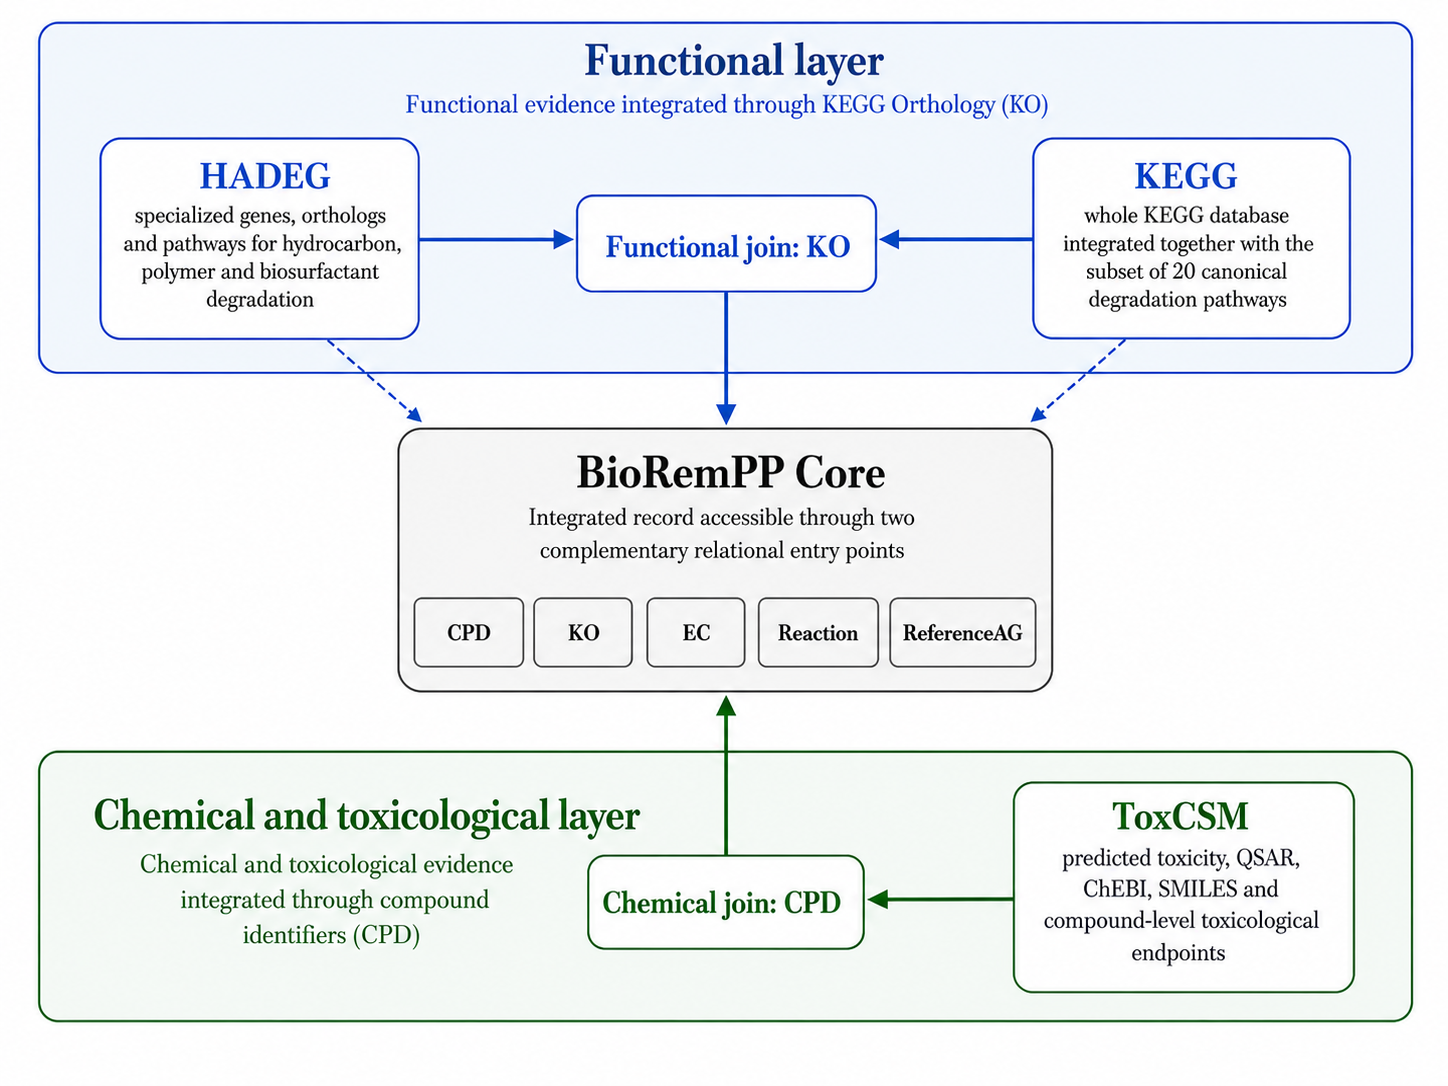
\includegraphics[width=\textwidth]{figures/chapter_03/fig_03_01_dual_axis.png}
\caption{Modelo de organização relacional do banco \biorempp{} baseado nas entidades KO e CPD. Os identificadores \gls{ko} relacionam as evidências funcionais, enquanto os identificadores \gls{cpd} relacionam as informações químicas e toxicológicas.}
\label{fig:c1-dualaxis}
\end{figure}

A manutenção das duas entidades decorre da estrutura das fontes integradas. A evidência funcional é organizada por grupos de ortologia KEGG, números EC e reações, enquanto as predições toxicológicas são indexadas por estrutura molecular. A conversão de todas as evidências para uma única chave exigiria relações que não estão disponíveis para todos os registros e poderia eliminar informações preservadas pelas fontes originais.

KO e CPD constituem, portanto, pontos de entrada complementares para consulta. O primeiro permite recuperar evidências relacionadas a funções gênicas e transformações enzimáticas. O segundo permite recuperar informações associadas ao composto, incluindo sua proveniência institucional e suas predições toxicológicas. Essa organização não pressupõe correspondência unívoca entre grupo de ortologia e composto.

\subsection{Estados de suporte relacional}

A construção da tabela central parte do universo de chaves
\texttt{cpd}--\texttt{ko}--\texttt{referenceAG}. Essas chaves são obtidas de
três origens: relações composto--EC--KO, relações composto--reação--KO e
associações composto--KO acrescentadas por curadoria. Cada chave é expandida
de acordo com as relações disponíveis no snapshot versionado do KEGG usado
na execução.

As chaves são classificadas em seis estados de suporte relacional, definidos
pela completude e pela origem das relações recuperadas
(Tabela~\ref{tab:c1-support-stages}). Os três primeiros estados resultam em
registros com número EC e reação preenchidos, embora usem caminhos distintos
de confirmação. Os dois estados seguintes preservam associações sustentadas
apenas por número EC ou por reação. O último mantém a associação curada entre
composto e KO quando as relações consultadas não permitem resolver nenhum
desses campos.

\begin{table}[htbp]
\centering
\caption{Estados de suporte usados na expansão das chaves
\texttt{cpd}--\texttt{ko}--\texttt{referenceAG}. Os identificadores internos
permitem relacionar as categorias descritas aos registros produzidos
pelo pipeline.}
\label{tab:c1-support-stages}
\small
\begin{tabularx}{\textwidth}{@{}p{3.2cm}p{2.8cm}Xll@{}}
\toprule
\textbf{Estado de suporte}
& \textbf{Identificador}
& \textbf{Critério de construção}
& \textbf{EC}
& \textbf{Reação} \\
\midrule

Mapeamento denso
& \texttt{dense}
& O KO possui número EC e reação, e a relação entre ambos é sustentada pelos
links EC--reação consultados.
& Preenchido
& Preenchida \\

Mapeamento denso alternativo
& \texttt{fallback\_dense}
& O KO possui número EC e reação, mas a combinação entre ambos não foi
confirmada pela relação direta EC--reação.
& Preenchido
& Preenchida \\

Mapeamento por ponte do composto
& \texttt{compound\_bridge}
& As relações do composto com número EC ou reação, combinadas às relações do
KO, sustentam a associação funcional.
& Preenchido
& Preenchida \\

Suporte apenas por EC
& \texttt{ec\_only}
& Existe suporte entre KO e número EC, mas nenhuma reação compatível foi
recuperada.
& Preenchido
& \texttt{NA} \\

Suporte apenas por reação
& \texttt{reaction\_only}
& Existe suporte entre KO e reação, mas nenhum número EC compatível foi
recuperado.
& \texttt{NA}
& Preenchida \\

Sem suporte nas relações consultadas
& \texttt{unsupported}
& A associação curada entre composto e KO não possui suporte para número EC
ou reação nos conjuntos de links KEGG consultados.
& \texttt{NA}
& \texttt{NA} \\

\bottomrule
\end{tabularx}
\end{table}

A nulabilidade de \texttt{ec}, \texttt{reaction} e
\texttt{reaction\_description} integra o contrato semântico do banco. O
pipeline não infere valores para completar relações ausentes. Uma linha
parcial indica que a associação entre composto e KO foi preservada, mas o
snapshot consultado não sustentou a resolução completa da transformação
enzimática.

O estado \texttt{unsupported} indica ausência de suporte nos conjuntos de
links KEGG consultados. Essa classificação não demonstra ausência de evidência
biológica em outras fontes nem exclui a possibilidade de que a relação seja
incorporada em versões posteriores do KEGG.

% -----------------------------------------------------------------------------
\section{Esquema de dados e identificadores interoperáveis}
\label{sec:c1-schema}
% -----------------------------------------------------------------------------

A tabela central BioRemPP possui 11 campos ordenados
(Tabela~\ref{tab:c1-schema}). O arquivo público é exportado em formato CSV,
com codificação UTF-8, delimitador ponto e vírgula, campos textuais entre
aspas duplas e \texttt{NA} como representação de valores ausentes. A ordem,
o tipo e a semântica desses campos constituem o contrato público do banco.

\begin{table}[htbp]
\centering
\caption{Esquema de dados da tabela central BioRemPP v1.1.0.}
\label{tab:c1-schema}
\small
\begin{tabularx}{\textwidth}{@{}llX@{}}
\toprule
\textbf{Campo} & \textbf{Tipo} & \textbf{Descrição} \\
\midrule

\texttt{cpd}
& Caractere
& Identificador KEGG Compound, formado pela letra C seguida de cinco
algarismos. \\

\texttt{compoundclass}
& Caractere
& Classe química atribuída segundo vocabulário controlado. \\

\texttt{ko}
& Caractere
& Identificador KEGG Orthology, formado pela letra K seguida de cinco
algarismos. \\

\texttt{ec}
& Caractere
& Número EC (\textit{Enzyme Commission}); campo que admite valor ausente. \\

\texttt{reaction}
& Caractere
& Identificador KEGG Reaction, formado pela letra R seguida de cinco
algarismos; campo que admite valor ausente. \\

\texttt{reaction\_description}
& Caractere
& Descrição textual da reação; permanece \texttt{NA} quando
\texttt{reaction} não está preenchido. \\

\texttt{referenceAG}
& Caractere
& Código da fonte institucional associada ao composto. \\

\texttt{compoundname}
& Caractere
& Nome do composto recuperado da lista KEGG Compound. \\

\texttt{genesymbol}
& Caractere
& Símbolo gênico associado ao identificador KO. \\

\texttt{genename}
& Caractere
& Descrição funcional associada ao identificador KO. \\

\texttt{enzyme\_activity}
& Caractere
& Descritor de atividade enzimática derivado de vocabulário curado e da
anotação funcional associada ao KO. \\

\bottomrule
\end{tabularx}
\end{table}

Os campos funcionais e químicos adotam identificadores de referência.
O campo \texttt{cpd} corresponde ao KEGG Compound, \texttt{ko} ao KEGG
Orthology, \texttt{reaction} ao KEGG Reaction e \texttt{ec} à nomenclatura
da \gls{ec}. Essa organização evita a criação de identificadores específicos
do BioRemPP para entidades que já possuem referências públicas estabelecidas.

No conjunto complementar ToxCSM, os identificadores ChEBI e as representações
\gls{smiles} preservam a ligação com recursos de quimioinformática. As
estruturas moleculares são mantidas em formato legível por máquina, permitindo
seu processamento por ferramentas externas sem conversão para um identificador
próprio do \biorempp{}.

O uso de identificadores públicos e formatos legíveis por máquina contribui
para a interoperabilidade e a reutilização previstas pelos princípios
\gls{fair}, discutidos na Seção~\ref{sec:fund-fair}. Essas propriedades
também dependem da consistência sintática dos valores. Os formatos de KO,
composto, reação e número EC são verificados durante a aquisição e a
normalização dos dados e novamente após a exportação do arquivo público.

\subsection{Nulabilidade e descrição das reações}

Os campos \texttt{ec}, \texttt{reaction} e
\texttt{reaction\_description} admitem valores ausentes como parte prevista
do modelo de dados. Quando um identificador de reação está presente, sua
descrição é recuperada da lista de reações do KEGG. Quando
\texttt{reaction} permanece \texttt{NA}, o campo
\texttt{reaction\_description} também recebe \texttt{NA}.

Essa dependência impede que uma descrição seja associada a um identificador
ausente. Também permite distinguir uma ausência prevista pelo modelo de uma
falha de preenchimento ou exportação. As frequências de valores ausentes e a
cobertura das descrições de reação observadas na versão 1.1.0 são apresentadas
na Seção~\ref{sec:c1-resultados}.

\subsection{Estrutura denormalizada e interpretação das cardinalidades}

A tabela central adota uma estrutura plana e denormalizada. Cada linha
representa uma combinação entre composto, classe química, referência
institucional, KO, número EC e reação. O número total de linhas, portanto,
não corresponde ao número de entidades únicas presentes no banco.

Consultas em nível de composto, KO, número EC ou reação devem considerar
valores distintos. A repetição de um identificador em diferentes linhas pode
resultar de sua associação a múltiplas classes químicas, referências
institucionais ou transformações enzimáticas e não indica, por si só, uma
duplicação inconsistente.

A inclusão de números EC e reações aumenta o número de combinações
representadas na tabela. Um par composto--KO que ocupava uma única linha em
uma versão anterior pode originar vários registros quando está associado a
diferentes combinações EC--reação. Comparações entre versões devem considerar
tanto o número de linhas quanto as cardinalidades de cada entidade.

A estrutura denormalizada produz repetição controlada de valores, mas permite
o uso direto do arquivo em R, Python e planilhas, sem reconstruir previamente
as relações em tabelas normalizadas. Os efeitos quantitativos dessa decisão
sobre a evolução entre as versões 1.0.0 e 1.1.0 são apresentados na
Seção~\ref{sec:c1-resultados}.

% -----------------------------------------------------------------------------
\section{Pipeline Snakemake}
\label{sec:c1-snakemake}
% -----------------------------------------------------------------------------

O banco foi produzido por um pipeline implementado em
Snakemake~\citep{molder2025snakemake}. O fluxo foi modelado como um
\gls{dag}, no qual são explicitadas as dependências entre entradas,
transformações e saídas. Essa organização permite executar novamente apenas
as etapas afetadas por alterações nos dados ou nos parâmetros, preservando os
resultados intermediários que permanecem válidos.

\subsection{Organização do pipeline}

O pipeline foi organizado em três responsabilidades: orquestração,
configuração e transformação dos dados. O Snakemake é responsável por controlar o encadeamento
das etapas e suas dependências, enquanto os parâmetros sujeitos a alteração
entre execuções, como caminhos, formatos de exportação e limites de
validação, foram mantidos em arquivos de configuração.

O esquema público, os identificadores aceitos e as entradas obrigatórias foram
mantidos em componentes versionados junto ao código. Essa separação permite
modificar parâmetros operacionais sem alterar a semântica dos dados
exportados. Mudanças no esquema, nas regras de identificação ou no conjunto
de entradas representam alterações no contrato público do banco e, por isso,
permanecem registradas no histórico do projeto.

As transformações foram implementadas como etapas independentes, cada uma com
entradas e saídas previamente definidas. Essa organização permitiu inspecionar
os resultados intermediários e evitou dependências diretas entre os scripts.
Operações compartilhadas de leitura, escrita, normalização de valores ausentes
e registro da execução foram centralizadas para manter o mesmo tratamento ao
longo do pipeline.


\subsection{Ambiente computacional reprodutível}

A geração e a validação do banco foram executadas por meio de containers
Docker versionados. O container de geração reuniu o Snakemake, o ambiente R e
os pacotes usados nas etapas de integração, enriquecimento, análise e
exportação. A validação baseada em Great Expectations foi executada em um
container Python independente, com suas próprias dependências.

A execução por meio do Docker preserva o ambiente de software usado na
construção do banco e reduz variações decorrentes do sistema operacional, das
bibliotecas instaladas localmente e das configurações.
Assim, o mesmo pipeline pode ser executado em diferentes ambientes
computacionais sem exigir a instalação manual de cada dependência.

A separação entre os containers de geração e validação também evita conflitos
entre os ambientes R e Python. Cada processo é executado com versões
previamente definidas de suas ferramentas e bibliotecas, permitindo reproduzir
as etapas com as mesmas dependências usadas na versão analisada.

As imagens Docker, as versões dos pacotes, os parâmetros de execução e os
comandos necessários para executar e reproduzir o pipeline estão descritos na
documentação oficial dos repositórios da organização BioRemPP, disponível em
\url{https://github.com/BioRemPP}.



\subsection{Etapas de execução}

O \gls{dag} foi organizado em seis etapas metodológicas
(Tabela~\ref{tab:c1-stages}). Etapas sem dependência direta puderam ser
executadas em paralelo, enquanto a construção da tabela central seguiu a ordem
estabelecida pelos resultados intermediários.

\begin{table}[htbp]
\centering
\caption{Etapas metodológicas do pipeline de geração, análise e validação do
banco BioRemPP.}
\label{tab:c1-stages}
\small
\begin{tabularx}{\textwidth}{@{}r l X@{}}
\toprule
\textbf{N.} & \textbf{Etapa} & \textbf{Finalidade} \\
\midrule

1 & Verificação e carregamento
& Confirmar a presença e a estrutura das entradas curadas antes do início das
transformações. \\

2 & Aquisição de dados e proveniência KEGG
& Recuperar as relações funcionais usadas na construção e registrar a versão
da fonte consultada. \\

3 & Integração relacional
& Formar as associações entre compostos, KOs, números EC, reações e
referências institucionais. \\

4 & Enriquecimento e exportação
& Acrescentar classes químicas, informações funcionais, descritores
enzimáticos e descrições de reação antes da exportação pública. \\

5 & Análise descritiva
& Calcular as cardinalidades, distribuições e tabelas cruzadas usadas para
caracterizar a versão produzida. \\

6 & Validação e relatório de execução
& Verificar a consistência funcional e estrutural dos resultados e registrar o
estado final da execução. \\

\bottomrule
\end{tabularx}
\end{table}

\begin{figure}[htbp]
\centering
\fbox{
    \parbox{0.85\textwidth}{
        \centering
        Representação esquemática do \gls{dag} do BioRemPP, com as etapas de
        verificação, geração, análise, validação e relatório.
        \vspace{2em}
    }
}
\caption{Grafo de dependências do pipeline Snakemake do banco
\biorempp{}. As arestas representam as dependências entre os resultados
produzidos em cada etapa.}
\label{fig:c1-dag}
\end{figure}

A integração relacional combinou os dados curados com as relações recuperadas
do KEGG. Os identificadores foram normalizados antes da formação do universo
\texttt{cpd}--\texttt{ko}--\texttt{referenceAG}. As combinações entre KO,
número EC e reação foram resolvidas segundo os estados de suporte relacional
descritos na Tabela~\ref{tab:c1-support-stages}. Os nomes dos compostos foram
obtidos da lista KEGG Compound recuperada na mesma execução.

As classes químicas foram acrescentadas após a formação das relações
funcionais. Compostos associados a mais de uma classe foram representados em
registros distintos. Os símbolos gênicos e as descrições funcionais foram
incorporados por correspondência com os identificadores KO.

Na etapa final, foram adicionadas as descrições das reações e os descritores de
atividade enzimática derivados do vocabulário curado e das anotações
funcionais. Os registros duplicados foram removidos antes da aplicação da
ordem final do esquema de dados.

Os resultados intermediários foram preservados entre as etapas. Essa
estratégia permitiu inspecionar as transformações e reiniciar o fluxo a partir
do primeiro estágio afetado por uma alteração, sem repetir aquisições ou
processamentos que permanecessem válidos.

\subsection{Produção das análises descritivas}

Após a exportação, o pipeline calculou as estatísticas usadas para caracterizar
o banco. Foram produzidas contagens de compostos, KOs, genes e descritores
enzimáticos distintos, além de distribuições, tabelas cruzadas e metadados da
execução.

Os resultados foram armazenados em formato estruturado e usados na descrição
quantitativa da versão e nos testes de consistência executados pela segunda
camada de validação. Os nomes dos arquivos, a estrutura dos diretórios e a
descrição detalhada das regras estão disponíveis na documentação oficial do
pipeline, mantida nos repositórios da organização BioRemPP.

% -----------------------------------------------------------------------------
\section{Validação ancorada no KEGG}
\label{sec:c1-validacao-kegg}
% -----------------------------------------------------------------------------

A primeira camada de validação foi incorporada ao \gls{dag} e comparou o banco exportado com um instantâneo das relações KEGG recuperadas durante a execução. Foram preservadas as relações entre KO e número EC, KO e reação, composto e número EC, composto e reação, e número EC e reação. O uso do mesmo instantâneo na geração e na validação evitou que alterações da fonte externa entre consultas interferissem na avaliação da versão produzida.

A análise das ausências verificou os registros com \texttt{NA} em \texttt{ec} ou \texttt{reaction}. Uma ausência foi considerada justificada quando as relações necessárias não estavam presentes no instantâneo consultado. Foi considerada inconsistente quando o KEGG continha suporte suficiente para preencher o campo, mas a relação não havia sido materializada no banco.

Os registros com número EC e reação preenchidos foram avaliados quanto ao suporte das combinações \texttt{(ko, ec, reaction)}. A política de união, identificada nos relatórios como \texttt{policy\_union}, aceitou as relações sustentadas por qualquer uma das estratégias densas usadas na construção do banco. O critério \texttt{strict5} exigiu concordância simultânea entre as cinco relações consultadas e foi usado como medida restritiva complementar, sem representar isoladamente a cobertura global da validação.

A proporção máxima de registros sem suporte foi definida antes da execução. A ausência de arquivos obrigatórios, falhas na aquisição das relações, erros de leitura ou ultrapassagem desse limite interromperam o fluxo. Os resultados quantitativos dessa avaliação são apresentados na Seção~\ref{sec:c1-resultados}, junto às demais métricas da versão 1.1.0.

% -----------------------------------------------------------------------------
\section{Validação estrutural e detecção de regressão}
\label{sec:c1-validacao-gx}
% -----------------------------------------------------------------------------

A segunda camada de validação foi implementada com Great Expectations~\citep{greatexpectations} e executada após a conclusão do pipeline Snakemake. O validador operou em modo somente leitura sobre o banco exportado, os metadados e os resultados analíticos. Seu objetivo foi verificar o contrato estrutural do arquivo público e a coerência entre os artefatos produzidos na mesma execução.

\subsection{Complementaridade entre as camadas}

As duas camadas avaliaram propriedades distintas. A validação ancorada no KEGG examinou a concordância das relações funcionais com a fonte externa usada na construção. O Great Expectations verificou o esquema de dados, os formatos dos identificadores, a nulabilidade dos campos, os vocabulários controlados e a unicidade dos registros. Também comparou as métricas recalculadas a partir do CSV com os resultados analíticos produzidos pelo pipeline.

Essa combinação evita que a aprovação dependa apenas de uma dimensão de qualidade. Um arquivo pode preservar a estrutura esperada e conter relações funcionais incompatíveis com o KEGG. Também pode manter relações biologicamente sustentadas e apresentar quebra na ordem das colunas, nos identificadores ou nas métricas derivadas.

\subsection{Consistência interna e regressão}

A validação analítica foi organizada em dois modos. O modo de consistência interna comparou o banco com as estatísticas produzidas pela mesma execução. Contagens, distribuições e sumários foram recalculados a partir do CSV e confrontados com os artefatos analíticos correspondentes.

O modo de detecção de regressão comparou as métricas da versão avaliada com uma linha de base versionada (\textit{baseline}). A comparação foi realizada sobre medidas derivadas, e não sobre a sequência bruta das linhas do CSV. Essa escolha impediu que mudanças sem efeito científico, como uma ordenação diferente dos registros, fossem classificadas como regressões.

As verificações foram classificadas em críticas e de aviso. Falhas críticas indicaram quebra do contrato necessário para publicação. Os avisos acompanharam variações de cardinalidade ou de vocabulário que exigiam revisão, mas cuja interpretação dependia do contexto da nova versão.

\begin{table}[htbp]
\centering
\caption{Dimensões avaliadas pela validação estrutural e analítica do BioRemPP.}
\label{tab:c1-validation-dimensions}
\small
\begin{tabularx}{\textwidth}{@{}lX@{}}
\toprule
\textbf{Dimensão} & \textbf{Verificação} \\
\midrule
Contrato do banco
& Ordem e presença das colunas, formatos dos identificadores, nulabilidade e unicidade dos registros. \\

Proveniência
& Presença e consistência dos metadados da fonte KEGG usada na construção. \\

Consistência interna
& Correspondência entre as métricas recalculadas a partir do CSV e os resultados analíticos da mesma execução. \\

Regressão
& Comparação das métricas derivadas com a linha de base aprovada para identificar mudanças não previstas. \\
\bottomrule
\end{tabularx}
\end{table}

Os artefatos hierárquicos foram convertidos em representações tabulares antes da aplicação das verificações. Essa etapa permitiu validar o banco, os metadados e as métricas com um conjunto uniforme de expectativas, sem incorporar a lógica de leitura de cada arquivo às próprias regras de validação.

\subsection{Controle de qualidade do validador}

O validador foi submetido a testes automatizados que cobriram execuções aprovadas e falhas representativas, incluindo ausência de arquivos, alteração do esquema de dados, inconsistência dos metadados e variações acima dos limites configurados. Esses testes verificaram o comportamento da ferramenta e reduziram o risco de que uma falha no próprio sistema de validação fosse interpretada como propriedade dos dados.

A configuração completa das expectativas, a composição da linha de base, os cenários de teste e os procedimentos de execução estão documentados nos repositórios oficiais da organização BioRemPP, disponíveis em \url{https://github.com/BioRemPP}.


% -----------------------------------------------------------------------------
\section{Resultados do componente}
\label{sec:c1-resultados}
% -----------------------------------------------------------------------------

A release v1.1.0 contém 123.543 linhas e 11 colunas. O banco reúne 384 compostos distribuídos em 12 classes químicas, 1.543 KOs, 994 números EC, 1.939 reações, 1.517 símbolos gênicos, 1.422 nomes de genes e 206 atividades enzimáticas. Todos os compostos estão associados a pelo menos um dos nove códigos de \texttt{referenceAG}. As predições do ToxCSM cobrem 370 compostos, correspondendo a 96,4\% do inventário.

\subsection{Construção e completude das relações}

O universo inicial continha 7.330 chaves distintas \texttt{cpd}--\texttt{ko}--\texttt{referenceAG}. As relações diretas baseadas em EC contribuíram com 3.461 chaves, as relações baseadas em reação contribuíram com 2.828 e a curadoria acrescentou 3.037; as sobreposições foram removidas antes da expansão.

O estado \texttt{dense} resolveu 4.752 chaves, equivalentes a 64,8\% do universo, e produziu 23.015 linhas. O estado \texttt{fallback\_dense} resolveu 162 das 2.578 chaves residuais e produziu 1.890 linhas. O estado \texttt{compound\_bridge} resolveu 1.158 das 2.416 chaves restantes e produziu 83.077 linhas. As 1.258 chaves residuais foram avaliadas para suporte parcial, gerando 1.105 linhas com EC e 503 com reação. Quarenta e quatro chaves permaneceram sem suporte nos links consultados. Antes da expansão por classes químicas e dos enriquecimentos finais, \texttt{merged\_compounds.rds} continha 109.634 linhas.

No arquivo público, 120.432 linhas possuem EC e reação, 2.150 possuem apenas EC, 888 possuem apenas reação e 73 apresentam os dois campos como \texttt{NA}. A diferença entre os números intermediários e finais decorre principalmente da expansão dos compostos associados a múltiplas classes químicas. O enriquecimento gênico, a filtragem de registros sem anotação e a remoção final de duplicatas completam a definição do arquivo público.

A comparação com os caches KEGG encontrou correspondência direta para 1.527 dos 1.543 KOs e para 169 dos 384 compostos. Os 215 compostos sem correspondência direta nos links em nível de composto permaneceram conectados por suporte baseado em KO ou por pares curados. Esse resultado evidencia a dependência da curadoria para manter no banco substâncias regulatoriamente prioritárias que não possuem cobertura equivalente nas relações públicas consultadas.

\subsection{Distribuição por classe química}

As classes com maior número de compostos são aromáticos (n=123), clorados (n=117), compostos contendo nitrogênio (n=115), poliaromáticos (n=98) e alifáticos (n=94). As demais classes são metais (n=29), inorgânicos (n=26), compostos contendo enxofre (n=20), organofosforados (n=13), organometálicos (n=9), halogenados (n=8) e organossulfurados (n=1). Como um composto pode receber mais de uma classe, a soma das contagens supera 384.

\begin{figure}[htbp]
\centering
\fbox{\parbox{0.75\textwidth}{\centering Gráfico de barras horizontais com as 12 classes químicas ordenadas pelo número de compostos únicos na release v1.1.0.\vspace{2em}}}
\caption{Distribuição dos compostos prioritários do banco \biorempp{} v1.1.0 por classe química.}
\label{fig:c1-classes}
\end{figure}

\subsection{Cobertura por referência institucional}

A ATSDR contém 191 compostos do inventário (49,7\%). As demais frequências são IARC2B, com 130 compostos (33,9\%); PSL, com 99 (25,8\%); EPC, com 91 (23,7\%); WFD, com 84 (21,9\%); EPA, com 83 (21,6\%); IARC1, com 56 (14,6\%); CONAMA, com 43 (11,2\%); e IARC2A, com 29 (7,6\%). Os percentuais somam mais de 100\% porque um composto pode ocorrer em várias fontes.

\begin{figure}[htbp]
\centering
\fbox{\parbox{0.75\textwidth}{\centering Diagrama de sobreposição entre os nove códigos de \texttt{referenceAG}, com ênfase nas interseções entre fontes institucionais.\vspace{2em}}}
\caption{Sobreposição de compostos entre as referências institucionais integradas no banco \biorempp{}.}
\label{fig:c1-agencias}
\end{figure}

\subsection{Famílias enzimáticas}

A amplitude de cada família foi medida pelo número de compostos distintos associados. As maiores coberturas foram observadas para desidrogenases, com 106 compostos; dioxigenases, com 88; monooxigenases, com 74; redutases, com 53; e citocromos P450, com 35.

A ordenação muda quando a métrica é a frequência de linhas. Citocromo P450 aparece em 17.729 registros, seguido por dioxigenases (11.414), hidrolases (7.818), desidrogenases (6.813) e redutases (6.314). A primeira métrica descreve a diversidade de compostos cobertos. A segunda reflete a participação de cada família na expansão por KO, EC, reação, classe e referência institucional.

\subsection{Métricas de validação}

A camada KEGG-anchored classificou como justificadas todas as 3.111 linhas com pelo menos um valor ausente entre EC e reação. Nenhuma linha foi classificada como incorreta. A política de união sustentou as 120.432 linhas densas, e nenhuma permaneceu sem suporte pelos modelos admitidos.

A execução do Great Expectations registrada em 28 de junho de 2026 aprovou os checkpoints crítico e de warning. O sumário registrou zero expectativas críticas falhas e zero expectativas de warning falhas (Tabela~\ref{tab:c1-validation-metrics}).

\begin{table}[htbp]
\centering
\caption{Métricas das duas camadas de validação da release v1.1.0.}
\label{tab:c1-validation-metrics}
\small
\begin{tabular}{@{}ll@{}}
\toprule
\textbf{Métrica} & \textbf{Valor} \\
\midrule
Linhas com \texttt{NA} em EC ou reação & 3.111 \\
Ausências classificadas como justificadas & 3.111 \\
Ausências classificadas como incorretas & 0 \\
Linhas densas avaliadas & 120.432 \\
\texttt{policy\_union} & 100,0\% \\
\texttt{strict5} & 2,42\% \\
Checkpoint crítico do GX & Aprovado \\
Checkpoint de warning do GX & Aprovado \\
Expectativas críticas falhas & 0 \\
Expectativas de warning falhas & 0 \\
\bottomrule
\end{tabular}
\end{table}

\subsection{Disponibilidade e licenciamento}

O banco integrado v1.1.0 está depositado no Zenodo sob licença CC BY 4.0, com DOI \href{https://doi.org/10.5281/zenodo.18905195}{10.5281/zenodo.18905195}. O código do pipeline e do validador está disponível na organização BioRemPP no GitHub sob licença Apache 2.0. O depósito associa os arquivos públicos à versão do KEGG, aos artefatos analíticos e aos relatórios de validação usados na release.

% -----------------------------------------------------------------------------
\section{Discussão específica do componente}
\label{sec:c1-discussao}
% -----------------------------------------------------------------------------

O recorte regulatório determina a função do banco. A incorporação de todos os compostos presentes no KEGG, HADEG ou ToxCSM produziria um inventário mais amplo, mas reduziria a relação direta com prioridades ambientais e sanitárias. O \biorempp{} mantém apenas os compostos associados às fontes institucionais selecionadas e registra essa proveniência no campo \texttt{referenceAG}. A sobreposição entre listas permanece acessível e pode ser usada como indicador de convergência entre jurisdições.

O modelo em dois eixos preserva a forma de organização das fontes. A evidência funcional pode ser consultada por KO sem exigir que todo ortólogo tenha um composto único correspondente. A evidência toxicológica pode ser consultada por CPD sem reduzir os 31 endpoints a uma anotação gênica. Essa separação também permite que uma consulta iniciada por composto recupere KOs associados e que uma consulta iniciada por KO recupere o conjunto de compostos ligados ao mesmo registro core.

A expansão relacional mostra que a ligação direta em nível de composto permanece incompleta no KEGG. Apenas 169 dos 384 compostos apresentaram correspondência direta nos conjuntos de links em nível de CPD. A preservação dos 215 compostos restantes dependeu de suporte por KO ou de pares curados composto--KO. A curadoria evita excluir substâncias relevantes por uma limitação de cobertura da fonte funcional, mas cria uma dependência de manutenção manual que precisa ser reavaliada em releases futuras.

Os seis estados de suporte tornam essa heterogeneidade observável. Linhas densas, parciais e sem suporte não são tratadas como equivalentes. Os campos \texttt{ec} e \texttt{reaction} registram a completude disponível no snapshot, e os relatórios de validação verificam se as ausências correspondem aos links recuperados. Essa política é preferível ao preenchimento inferido porque permite que o usuário diferencie uma relação confirmada de uma associação preservada por curadoria.

O schema denormalizado favorece o uso em ferramentas tabulares, mas exige interpretação adequada da cardinalidade. As 123.543 linhas representam a expansão de 384 compostos por classes, referências, KOs, números EC e reações. Contagens científicas em nível de entidade devem usar valores distintos. A publicação conjunta das estatísticas de compostos, KOs, enzimas e genes reduz o risco de interpretar o número bruto de linhas como tamanho do inventário químico.

A validação em duas camadas cobre propriedades que não podem ser avaliadas pelo mesmo mecanismo. O cache KEGG verifica a fidelidade das relações funcionais usadas na construção. O Great Expectations verifica o contrato do arquivo, a coerência dos artefatos derivados e a estabilidade em relação à baseline. A aprovação das duas camadas na release v1.1.0 mostra que o arquivo público reproduz as métricas declaradas e que as relações densas atendem à política de suporte definida pelo pipeline. A separação entre execução, proveniência e validação também aproxima o componente dos princípios de análise sustentável discutidos por~\citet{molder2025snakemake}.

A baseline de regressão precisa ser atualizada de forma controlada quando uma mudança intencional altera as métricas da release. A igualdade com uma versão anterior não deve impedir correções ou expansão do banco. Seu papel é tornar a mudança explícita e exigir revisão antes que o novo perfil analítico seja aceito como referência.

A tabela core sustenta os demais componentes do ecossistema. O \gls{dbx} usa o schema e os identificadores para navegação e consulta. O \gls{bws} usa as relações entre compostos e KOs para analisar dados submetidos pelo usuário. O \gls{cli} depende da estabilidade dos arquivos públicos para integrar o recurso a workflows externos. A reutilização desses componentes depende da manutenção coordenada do contrato de dados, do pipeline e dos relatórios de validação.

% =============================================================================
% =============================================================================
% CAPÍTULO 4 --- COMPONENTE 2: BIOREMPP DATABASE EXPLORER (DBX)
% =============================================================================
% =============================================================================
\chapter{Componente 2: BioRemPP Database Explorer (DBX)}
\label{cap:comp2}

% -----------------------------------------------------------------------------
\section{Motivação e escopo do componente}
\label{sec:c2-motivacao}
% -----------------------------------------------------------------------------

O banco integrado descrito no Capítulo~\ref{cap:comp1} é distribuído em
arquivos CSV e XLSX associados a uma versão publicada. Esse formato preserva
o conteúdo científico, permite sua reutilização programática e mantém o
registro das entidades e relações incorporadas ao banco. Entretanto, a
distribuição por arquivos não oferece, isoladamente, uma camada de consulta
interativa.

A exploração direta desses arquivos exige conhecimento prévio do esquema de
dados e das relações entre compostos, KOs, números EC, reações, vias,
referências institucionais e predições toxicológicas. A estrutura
denormalizada também exige que o pesquisador diferencie o número de linhas das
cardinalidades de cada entidade e reconstrua localmente associações
muitos-para-muitos. Essas operações podem ser executadas em R, Python ou
sistemas de banco de dados, mas dependem da escrita de código e da preparação
do ambiente de análise. O \gls{dbx} fornece uma camada de acesso ao conteúdo integrado sem substituir
os arquivos científicos publicados. A aplicação organiza a evidência em uma
estrutura orientada à consulta e a disponibiliza por uma interface web. O
usuário pode pesquisar entidades, aplicar filtros e percorrer relações entre
compostos, grupos de ortologia KEGG, vias metabólicas, classes químicas,
referências institucionais e predições toxicológicas sem reconstruir
localmente as associações do banco.

A navegação é centrada no composto porque as informações recuperadas pela
interface convergem para as substâncias incluídas no universo institucional do
BioRemPP. Essa organização não reduz todas as evidências a um único
identificador. Os identificadores \gls{cpd} preservam a referência química e
a ligação com as predições toxicológicas, enquanto os identificadores
\gls{ko} conectam os compostos às anotações funcionais do HADEG e do
subconjunto KEGG Degradation. CPD e KO permanecem, portanto, como entidades
complementares de consulta. A aplicação disponibiliza módulos dedicados a compostos, classes químicas,
genes e KOs, vias e toxicidade. Esses módulos permitem consultar registros
individuais e percorrer entidades relacionadas. O componente também reúne
oito análises guiadas que formalizam perguntas sobre amplitude de anotação
funcional, toxicidade predita, classificação institucional e conectividade
entre compostos, KOs e vias. Os filtros e parâmetros dessas análises tornam
explícito o recorte aplicado a cada resultado.

O \gls{dbx} não recebe conjuntos de dados do usuário para processamento. Sua
função é consultar o acervo integrado e versionado. Essa característica o
distingue do \gls{bws}, apresentado no Capítulo~\ref{cap:comp3}, que processa
anotações funcionais submetidas pelo usuário para produzir perfis associados
às amostras analisadas. O Database Explorer opera sobre um conjunto de
referência previamente construído, enquanto o Web Service aplica as relações
do BioRemPP a dados externos. O escopo do \gls{dbx} é exploratório. As associações exibidas representam
registros curados, relações recuperadas de bases públicas e predições
computacionais. Elas sustentam a formulação de hipóteses e a priorização de
entidades para análises posteriores, mas não confirmam a degradação de um
composto nem sua toxicidade em condições ambientais.

A presença de uma substância em uma fonte institucional também não constitui
avaliação jurídica ou determinação de risco para um local específico. Da
mesma forma, a ausência de uma relação na interface pode refletir os limites
de cobertura ou a versão das fontes integradas. A interpretação dos resultados
deve considerar a proveniência, a natureza da evidência e os critérios usados
na construção do banco.

% -----------------------------------------------------------------------------
\section{Arquitetura e organização dos dados}
\label{sec:c2-arquitetura}
% -----------------------------------------------------------------------------

O banco integrado é publicado em arquivos CSV e XLSX com estrutura
denormalizada, adequada à distribuição, à preservação e ao processamento
programático. Essa organização mantém no mesmo arquivo as combinações entre
compostos, KOs, números EC, reações, classes químicas e referências
institucionais. Seu uso direto pela aplicação exigiria ler, filtrar e agrupar
essas combinações a cada requisição.

O BioRemPP Database Explorer usa um banco SQLite derivado dos conjuntos
publicados. Essa representação mantém apenas as estruturas necessárias às
consultas da aplicação e permite selecionar, ordenar, agrupar e paginar os
registros sem processar novamente a tabela denormalizada. O formato em arquivo
único também reduz os componentes necessários para disponibilizar o banco no
ambiente de execução. A camada interna de API orquestra o acesso entre a interface web e o SQLite. A
interface envia os parâmetros de busca, filtragem e paginação, enquanto a API
executa as consultas correspondentes e retorna os resultados em estruturas
consumidas pelos módulos da aplicação. O frontend não acessa diretamente o
banco nem processa os arquivos CSV e XLSX.

Antes da inicialização, o servidor verifica a presença do arquivo SQLite e das
tabelas exigidas pela aplicação. O banco é aberto em modo somente leitura, o
que impede alterações durante as consultas. A API organiza o acesso aos dados
por domínio, com operações específicas para compostos, genes e KOs, vias,
toxicidade, metadados e análises guiadas.

\subsection{Construção do banco SQLite}

A construção do SQLite usa como entradas a tabela central BioRemPP, o HADEG,
o subconjunto KEGG Degradation e o ToxCSM. As informações do HADEG e do
subconjunto KEGG Degradation são associadas à tabela central por KO, enquanto
as predições toxicológicas são relacionadas por CPD.

O processo verifica os identificadores necessários às associações e agrupa os
valores distintos de cada entidade. Os registros são reorganizados por
composto, KO, via, referência institucional e endpoint toxicológico. Também
são preservadas as combinações entre composto, KO, número EC, reação, via e
fonte necessárias às páginas de detalhe e às análises guiadas. O SQLite é reconstruído a partir dos conjuntos correspondentes a cada versão
do banco. Após a carga, verificações de consistência comparam as contagens
armazenadas nos resumos por entidade com os registros que lhes dão origem. Os
resultados quantitativos da construção e dessas verificações são apresentados
na Seção~\ref{sec:c2-resultados}. A Figura~\ref{fig:c2-data-architecture} resume o fluxo entre os conjuntos de
entrada, o banco SQLite, a API interna e a interface web.

\begin{figure}[htbp]
\centering
\fbox{
    \parbox{0.92\textwidth}{
        \centering

        \textbf{Conjuntos de entrada}\\[0.4em]
        BioRemPP central
        \quad HADEG
        \quad KEGG Degradation
        \quad ToxCSM

        \vspace{0.6em}
        $\downarrow$

        \vspace{0.4em}
        \textbf{Associação por KO e CPD}\\
        verificação dos identificadores e agrupamento dos registros

        \vspace{0.6em}
        $\downarrow$

        \vspace{0.4em}
        \textbf{Banco SQLite}\\
        resumos por entidade, mapeamentos e relações contextuais

        \vspace{0.6em}
        $\downarrow$

        \vspace{0.4em}
        \textbf{API interna}\\
        busca, filtragem, ordenação, paginação e análises guiadas

        \vspace{0.6em}
        $\downarrow$

        \vspace{0.4em}
        \textbf{Interface web}\\
        exploradores, páginas de detalhe e visualizações

        \vspace{0.8em}
    }
}
\caption{Arquitetura de dados do BioRemPP Database Explorer. Os conjuntos de
entrada são associados por KO ou CPD e reorganizados em um banco SQLite. A
API interna consulta esse banco e fornece os resultados apresentados pela
interface web. \todo{ELABORAR DIAGRAMA}} 
\label{fig:c2-data-architecture}
\end{figure}

\todo{ELABORAR DIAGRAMA}

Os arquivos publicados e o SQLite atendem a finalidades distintas. Os
arquivos CSV e XLSX preservam e distribuem o conteúdo integrado, enquanto o
SQLite fornece uma representação compacta para as operações da aplicação.
Como o banco de consulta pode ser reconstruído a partir das entradas
versionadas, ele não substitui o artefato científico depositado.

\subsection{Organização dos dados e consulta pela API}

O banco SQLite contém estruturas voltadas a quatro tipos de operação:
consultas por entidade, recuperação de associações, reconstrução do contexto
funcional e acesso às predições toxicológicas. Essa organização evita
recalcular, durante cada consulta, as agregações presentes na tabela
denormalizada.

A Tabela~\ref{tab:c2-data-groups} resume a função desses grupos. Os nomes
completos das tabelas, os campos, os tipos e os índices permanecem registrados
na documentação oficial do projeto.

\begin{table}[htbp]
\centering
\caption{Grupos de dados usados pelo BioRemPP Database Explorer.}
\label{tab:c2-data-groups}
\small
\begin{tabularx}{\textwidth}{@{}p{3.8cm}X@{}}
\toprule
\textbf{Grupo} & \textbf{Função na aplicação} \\
\midrule

Resumos por entidade
& Mantêm uma representação por composto, KO ou via e as contagens usadas em
buscas, filtros e ordenações. \\

Mapeamentos entre entidades
& Registram as associações entre compostos, símbolos gênicos, vias e
referências institucionais. \\

Contexto funcional
& Preserva as combinações entre CPD, KO, atividade enzimática, número EC,
reação, via e fonte. \\

Predições e metadados
& Armazena os valores por combinação composto--endpoint e as informações de
identificação e proveniência associadas ao CPD. \\

\bottomrule
\end{tabularx}
\end{table}

Os resumos por entidade fornecem os campos usados nas listagens e nos filtros
da interface. Para os compostos, esses campos incluem nome, classe química e
contagens de KOs, vias e referências institucionais. A classe química funciona
como atributo de exibição, agrupamento e filtragem; ela não participa das
associações funcionais estabelecidas por KO ou CPD.

As associações entre compostos, KOs, vias e referências institucionais são
mantidas em estruturas próprias. O contexto das associações funcionais
preserva as combinações necessárias para recuperar números EC, reações,
atividades enzimáticas e vias relacionadas a cada composto. As predições
toxicológicas permanecem organizadas por composto e endpoint.

A Figura~\ref{fig:c2-relational-model} apresenta uma visão conceitual dessas
associações. Campos auxiliares e estruturas exclusivas da implementação foram
omitidos.

\begin{figure}[htbp]
\centering
\fbox{
    \parbox{0.88\textwidth}{
        \centering

        \textbf{KOs e anotações funcionais}

        \vspace{0.5em}
        $\updownarrow$

        \vspace{0.5em}
        \textbf{Composto}\\
        CPD, nome, classe química e contagens associadas

        \vspace{0.5em}

        $\swarrow$
        \hspace{4em}
        $\downarrow$
        \hspace{4em}
        $\searrow$

        \vspace{0.5em}

        \textbf{Vias}
        \hspace{3em}
        \textbf{Referências}
        \hspace{3em}
        \textbf{Toxicidade}

        \vspace{0.5em}

        associações por KO
        \hspace{2em}
        fontes institucionais
        \hspace{2em}
        endpoints por CPD

        \vspace{0.8em}
    }
}
\caption{Organização conceitual das consultas no banco SQLite. O composto
constitui o principal ponto de navegação, com associações a KOs, vias,
referências institucionais e endpoints toxicológicos. \todo{ELABORAR DIAGRAMA}}
\label{fig:c2-relational-model}
\end{figure}

Durante a execução, a API consulta exclusivamente o SQLite em modo somente
leitura. As operações são organizadas segundo os módulos da aplicação e
retornam apenas os registros necessários à página solicitada. Os arquivos de
origem não são carregados nem transformados durante essas requisições.

Os arquivos CSV e XLSX preservam o banco integrado para distribuição e
reutilização. O SQLite sustenta as consultas da aplicação, e a API controla o
acesso a essa representação. Cada formato permanece associado à função para a
qual foi produzido.

% -----------------------------------------------------------------------------
\section{Exploração e análises guiadas}
\label{sec:c2-exploracao}
% -----------------------------------------------------------------------------

O BioRemPP Database Explorer oferece duas modalidades complementares de
consulta ao banco integrado. Os módulos de exploração permitem selecionar a
entidade de interesse e combinar critérios de busca, filtragem e ordenação. As
análises guiadas, por sua vez, organizam perguntas previamente definidas e
aplicam procedimentos analíticos específicos a compostos, vias, genes e KOs.

Ambas as modalidades consultam a mesma representação SQLite e preservam a
navegação entre entidades relacionadas. A partir das listagens, o usuário pode
acessar páginas de detalhe que reúnem as associações disponíveis para o
registro selecionado. Essa organização permite iniciar a consulta por uma
entidade química, funcional ou toxicológica e prosseguir pelas relações
mantidas no banco.

\subsection{Módulos de exploração}

A interface organiza a consulta em cinco módulos, definidos pela unidade
representada na listagem principal: compostos, classes químicas, genes e KOs,
vias e toxicidade. Os módulos compartilham operações de busca, filtragem,
ordenação e acesso ao registro detalhado, mas apresentam recortes compatíveis
com a natureza da entidade consultada.

A Tabela~\ref{tab:c2-explorer-modules} resume a unidade de consulta, os
principais critérios de seleção e as relações recuperadas em cada módulo. Os
campos completos das interfaces permanecem descritos na documentação oficial
da aplicação.

\begin{table}[htbp]
\centering
\caption{Módulos de exploração do BioRemPP Database Explorer.}
\label{tab:c2-explorer-modules}
\footnotesize
\begin{tabularx}{\textwidth}{
    @{}
    p{2.4cm}
    p{2.8cm}
    p{4.7cm}
    X
    @{}
}
\toprule
\textbf{Módulo}
& \textbf{Unidade de consulta}
& \textbf{Critérios de seleção}
& \textbf{Relações recuperadas} \\
\midrule

Compostos
& Composto identificado por CPD
& Nome ou CPD, classe química, via, símbolo gênico, referência institucional
e intervalos de contagens.
& KOs, símbolos gênicos, vias, números EC, reações, referências
institucionais e predições toxicológicas. \\

Classes químicas
& Classe associada aos compostos
& Busca pelo nome da classe e seleção dos registros correspondentes.
& Compostos apresentados sob a mesma classe e respectivas medidas derivadas. \\

Genes e KOs
& KO, com símbolo e nome gênico associados
& Busca por KO, símbolo ou nome gênico e intervalo do número de compostos.
& Compostos, vias, atividades enzimáticas e anotações funcionais associadas. \\

Vias
& Combinação entre via e fonte
& Fonte de anotação, nome da via e intervalos de contagens.
& Compostos, KOs e símbolos gênicos associados à via selecionada. \\

Toxicidade
& Combinação entre composto e endpoint
& Grupo de endpoints, endpoint, categoria predita, classe química e intervalo
do valor numérico.
& Predição referente ao endpoint e ligação com o registro do composto. \\

\bottomrule
\end{tabularx}
\end{table}

O módulo de compostos constitui o ponto de entrada para consultas iniciadas
por uma substância específica. Cada registro corresponde a um CPD e apresenta
seu nome, sua classe química e medidas derivadas das associações disponíveis.
Os critérios de seleção permitem restringir o conjunto por anotações
funcionais, vias, referências institucionais e atributos químicos.

A página de detalhe reúne os KOs, símbolos gênicos, números EC, reações e vias
associados ao composto. O mesmo registro apresenta as referências
institucionais e as predições toxicológicas disponíveis, mantendo separadas
informações de natureza funcional, institucional e preditiva. A
Figura~\ref{fig:c2-compounds-explorer} apresenta uma captura representativa
desse módulo.

\begin{figure}[htbp]
\centering
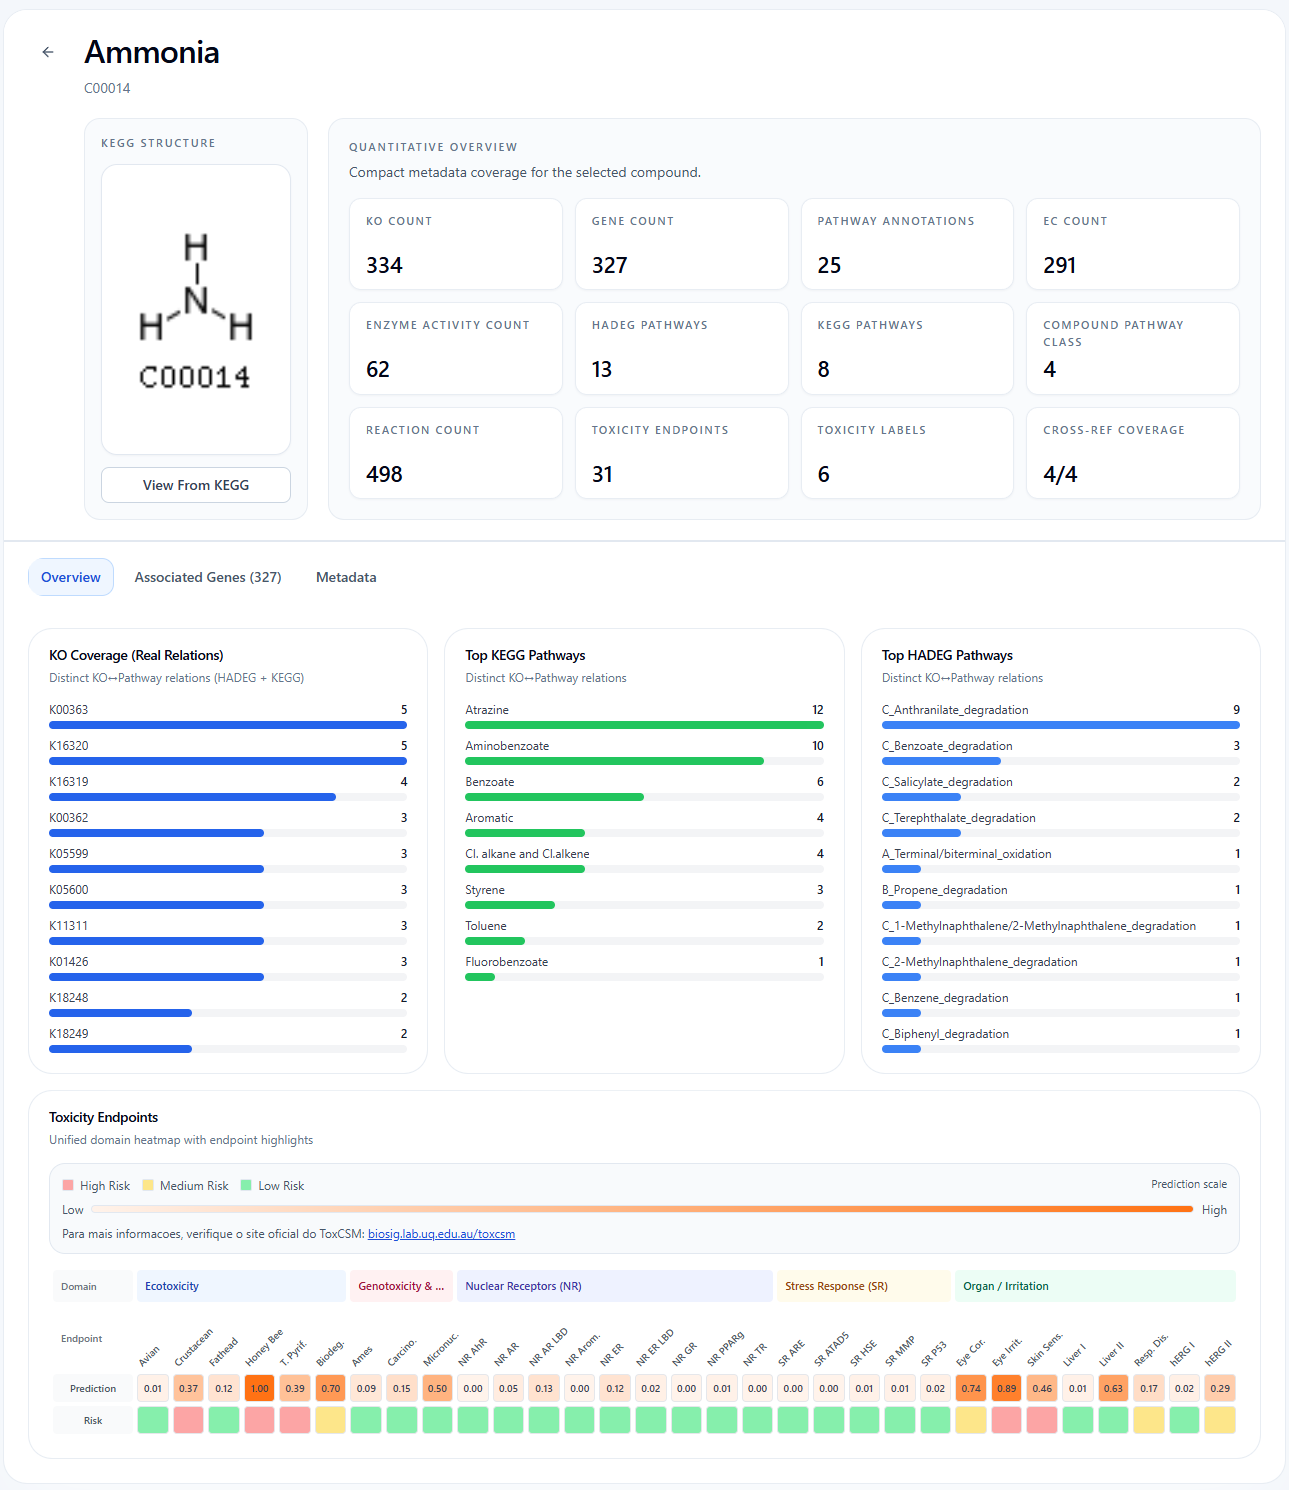
\includegraphics[width=\textwidth]
{figures/chapter_04/fig_04_compounds_explorer.png}
\caption{Módulo de exploração de compostos. A interface reúne critérios de
busca e filtragem com a listagem dos compostos e o acesso ao registro
detalhado de cada CPD.}
\label{fig:c2-compounds-explorer}
\end{figure}

O módulo de classes químicas organiza os compostos segundo o atributo de
classe apresentado pela interface. Essa perspectiva permite delimitar um
conjunto de substâncias antes da consulta aos respectivos registros
individuais. A classe é empregada na apresentação, no agrupamento e na
filtragem dos compostos, sem participar da definição das associações
funcionais estabelecidas por CPD e KO. A seleção de uma classe recupera os compostos apresentados sob o mesmo
rótulo e permite prosseguir para suas páginas de detalhe. A
Figura~\ref{fig:c2-compound-classes-explorer} exemplifica essa forma de
consulta.

\begin{figure}[htbp]
\centering
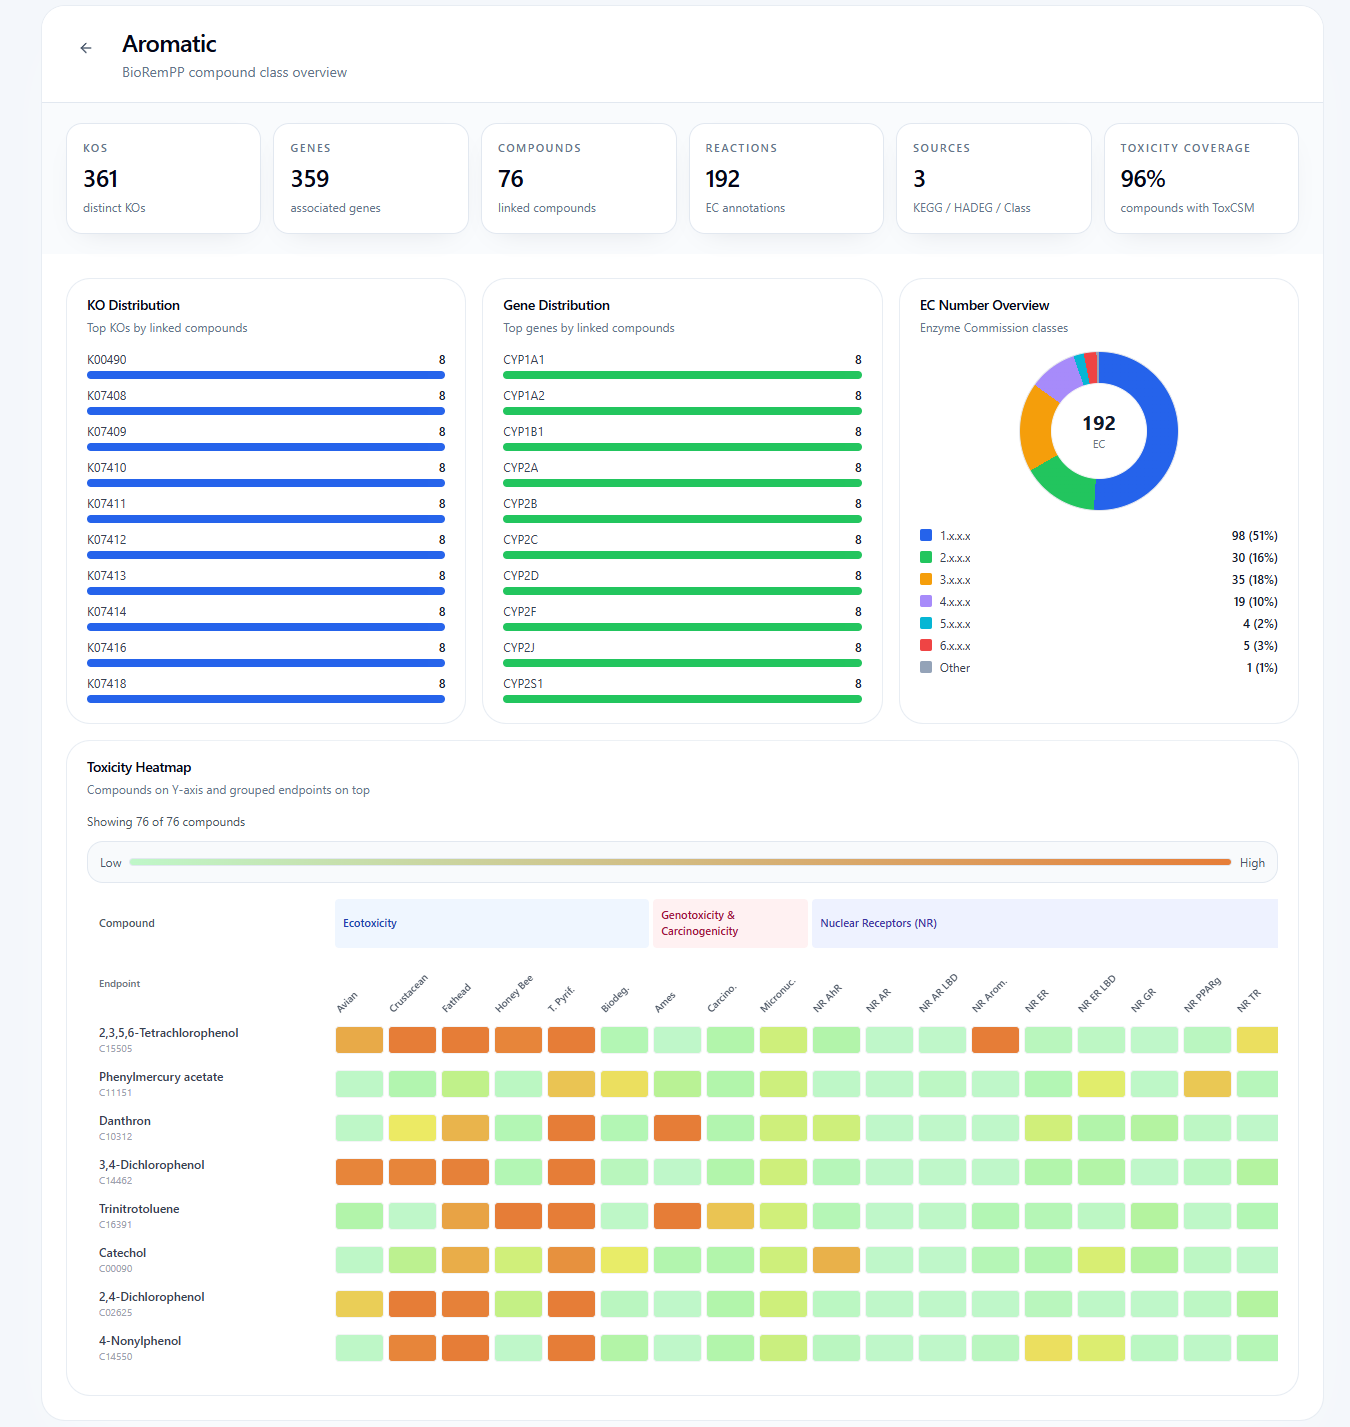
\includegraphics[width=\textwidth]
{figures/chapter_04/fig_04_compound_classes_explorer.png}
\caption{Módulo de exploração de classes químicas. A interface apresenta as
classes empregadas no agrupamento dos compostos e permite acessar os
registros correspondentes.}
\label{fig:c2-compound-classes-explorer}
\end{figure}

O módulo de genes e KOs permite iniciar a consulta por uma entidade funcional.
O KO constitui o identificador principal do registro, enquanto o símbolo e o
nome gênico fornecem descrições associadas. A listagem apresenta medidas
derivadas do número de compostos e vias relacionados a cada KO. A página de detalhe recupera os compostos, as vias, as atividades enzimáticas
e os números EC associados ao registro. As contagens apresentadas descrevem a
conectividade observada no banco e não representam expressão gênica, atividade
enzimática ou relevância metabólica. A
Figura~\ref{fig:c2-genes-ko-explorer} apresenta a organização desse módulo.

\begin{figure}[htbp]
\centering
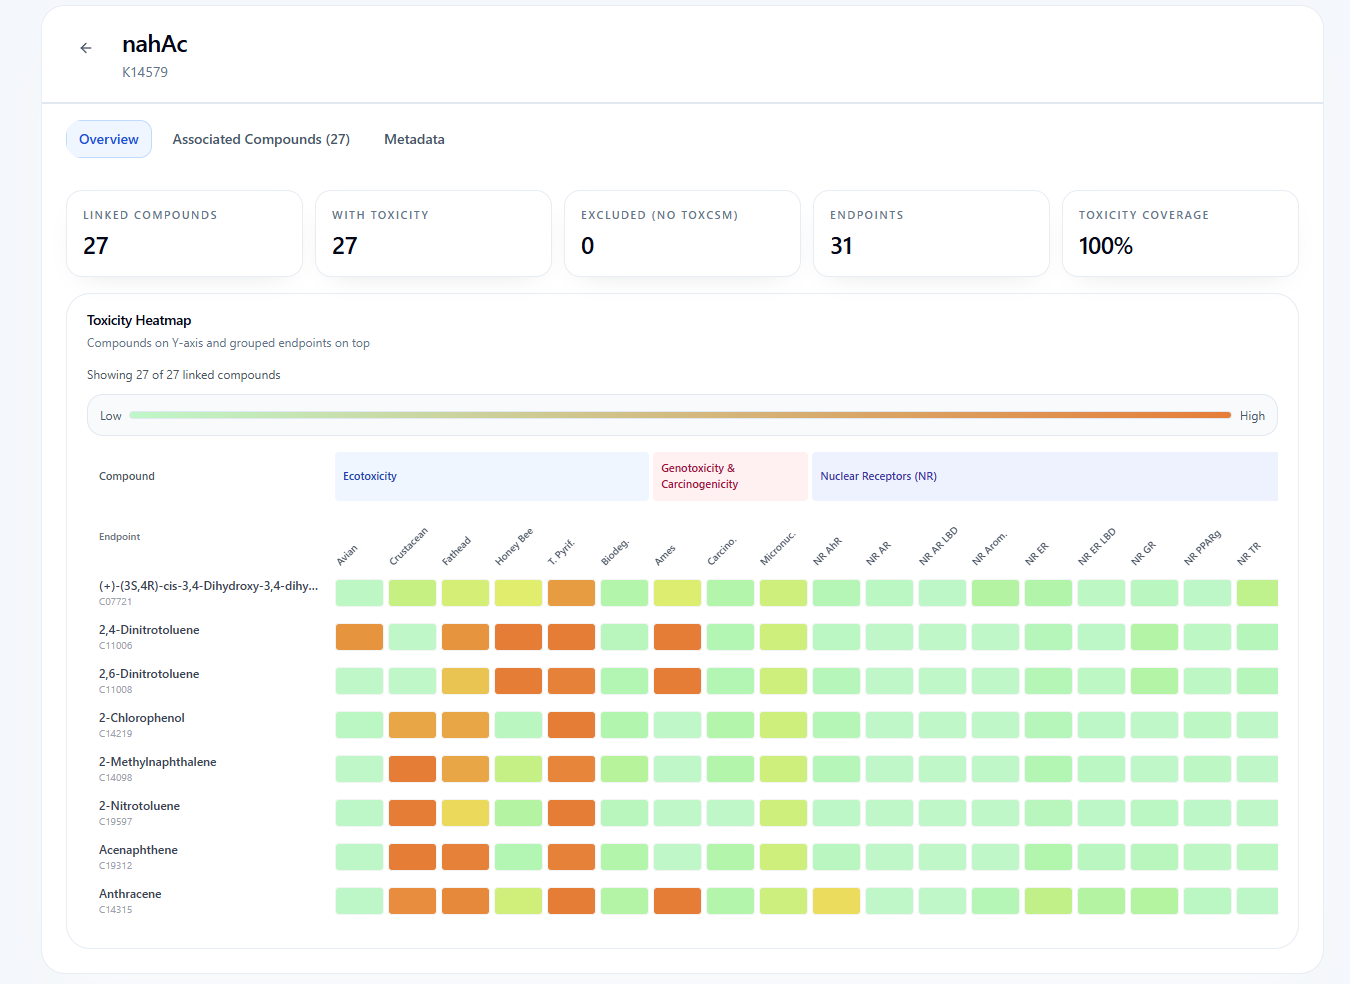
\includegraphics[width=\textwidth]
{figures/chapter_04/fig_04_genes_ko_explorer.png}
\caption{Módulo de exploração de genes e KOs. A interface permite consultar
grupos de ortologia KEGG e recuperar os compostos, as vias e as anotações
funcionais associadas.}
\label{fig:c2-genes-ko-explorer}
\end{figure}

O módulo de vias mantém a fonte de anotação como parte da identificação do
registro. Essa distinção permite consultar separadamente as vias provenientes
do HADEG, do subconjunto KEGG Degradation e das categorias adicionais
incorporadas à representação da aplicação, sem pressupor equivalência entre
seus critérios de organização. Para cada via, a interface apresenta medidas derivadas das associações com
compostos e anotações funcionais. A página de detalhe recupera os compostos e
KOs relacionados ao registro selecionado. Essas contagens não correspondem à
completude da via, ao fluxo metabólico ou à atividade dos seus componentes. A
Figura~\ref{fig:c2-pathways-explorer} exemplifica a consulta por via e fonte.

\begin{figure}[htbp]
\centering
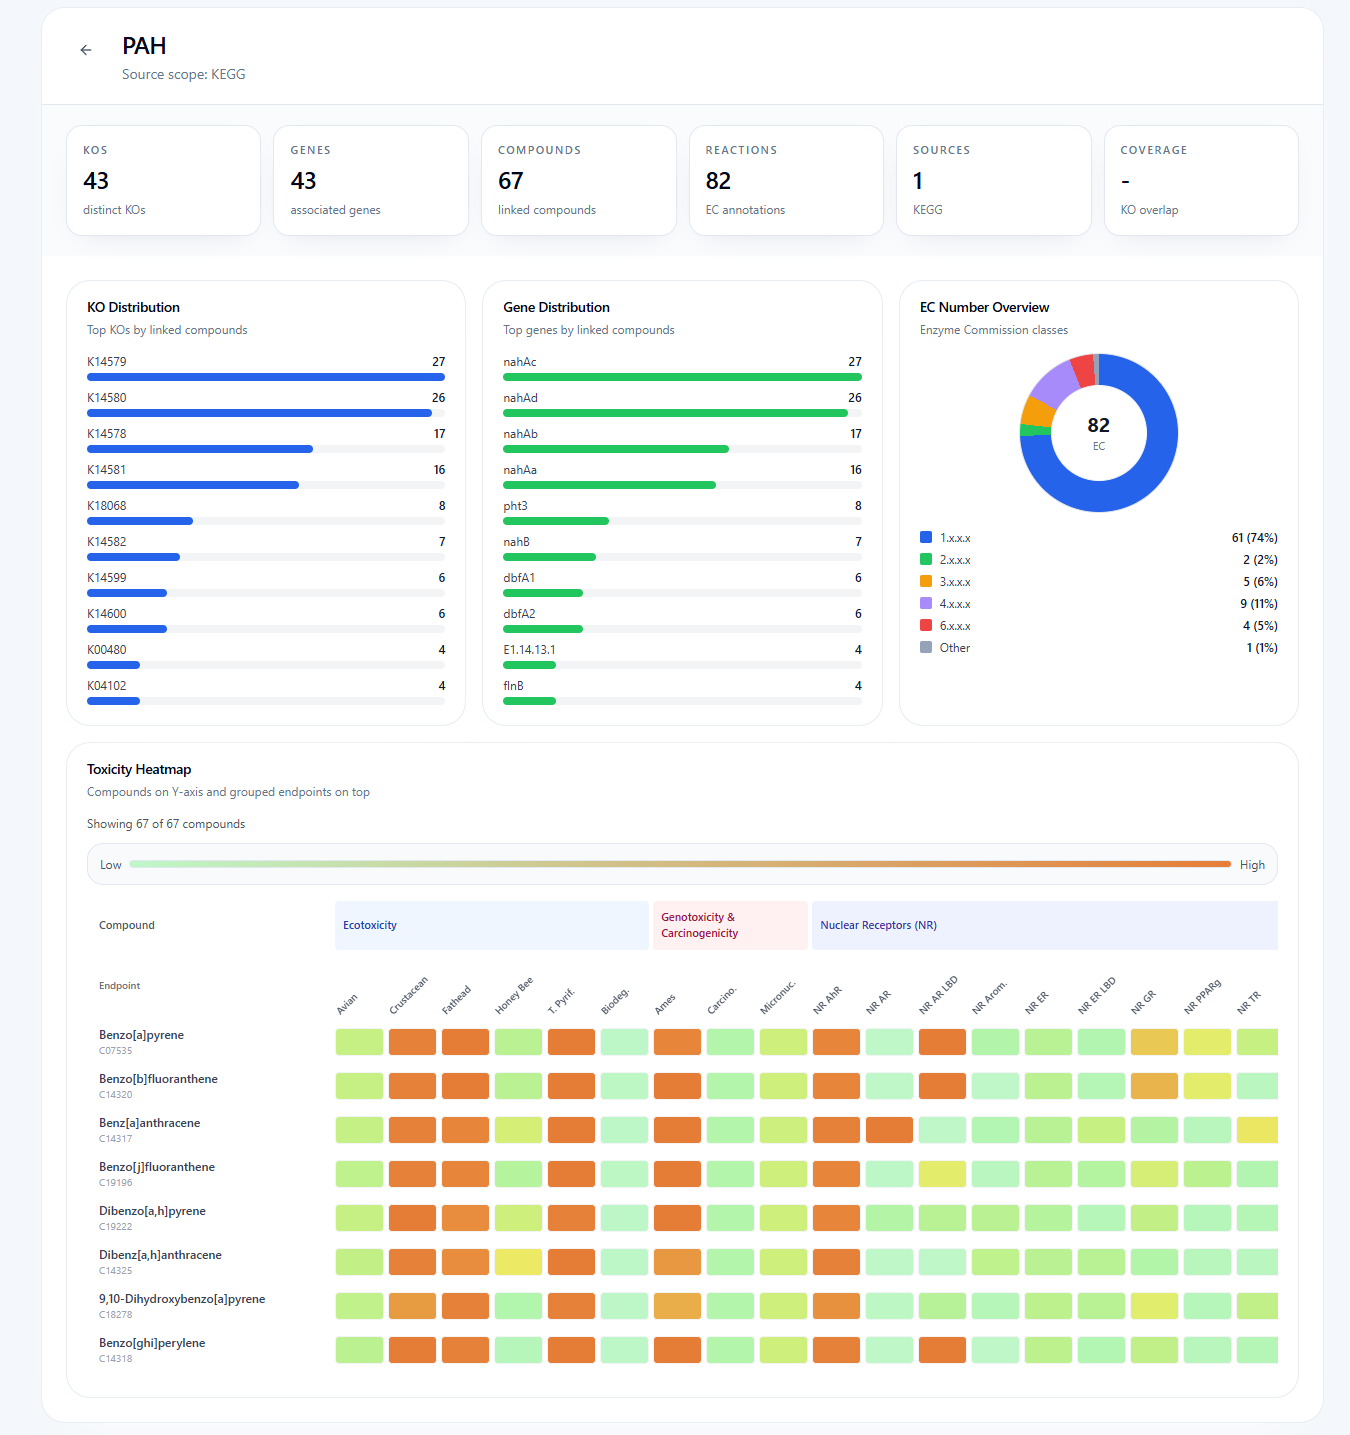
\includegraphics[width=\textwidth]
{figures/chapter_04/fig_04_pathways_explorer.png}
\caption{Módulo de exploração de vias. A interface preserva a fonte de
anotação e permite recuperar os compostos e KOs associados à via
selecionada.}
\label{fig:c2-pathways-explorer}
\end{figure}

O módulo de toxicidade adota a combinação entre composto e endpoint como
unidade de consulta. Os registros podem ser delimitados por grupo de
endpoints, endpoint específico, categoria predita, classe química e intervalo
numérico. A interpretação dos valores permanece condicionada ao endpoint
selecionado, pois os descritores representam propriedades toxicológicas
distintas. Cada resultado mantém a ligação com o CPD correspondente, o que permite
prosseguir para as informações funcionais e institucionais associadas ao
composto. Os valores apresentados resultam de modelos preditivos e não
equivalem a medidas experimentais de toxicidade. A
Figura~\ref{fig:c2-toxicity-explorer} apresenta uma consulta representativa
desse módulo.

\begin{figure}[htbp]
\centering
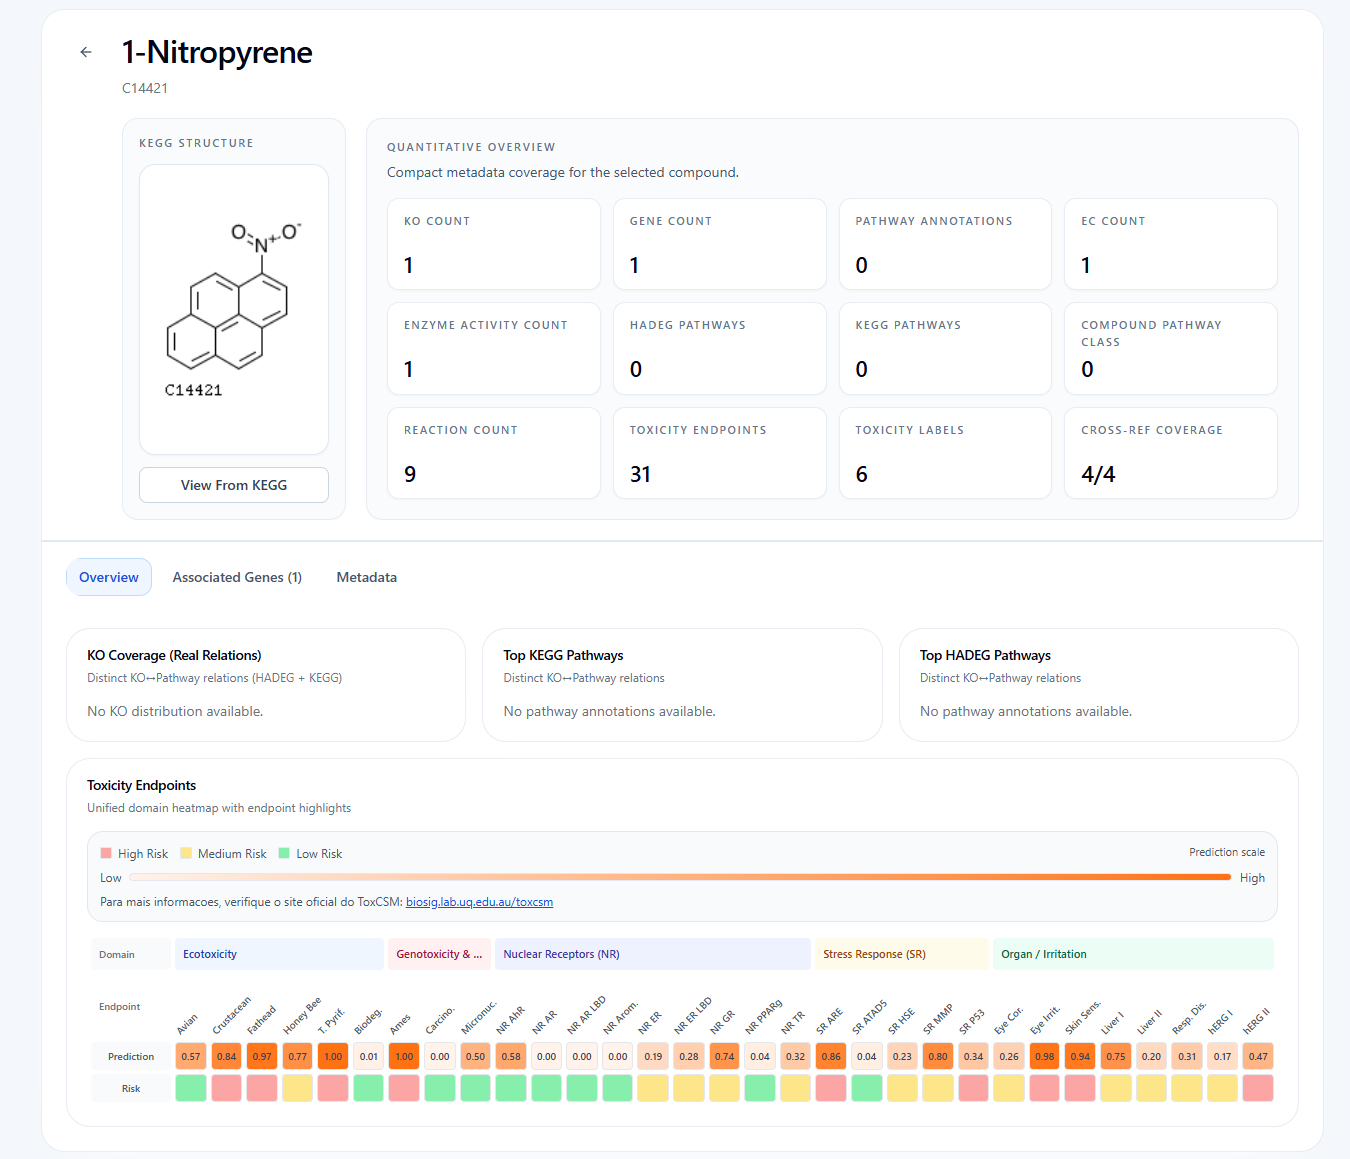
\includegraphics[width=\textwidth]
{figures/chapter_04/fig_04_toxicity_explorer.png}
\caption{Módulo de exploração de toxicidade. A interface organiza as
predições por composto e endpoint e preserva o vínculo com o registro do CPD
correspondente.}
\label{fig:c2-toxicity-explorer}
\end{figure}

A navegação entre as listagens e as páginas de detalhe conecta os cinco
módulos. Um composto recuperado por classe química ou endpoint toxicológico
pode ser examinado por suas associações com KOs e vias. De modo recíproco, uma
consulta iniciada por KO ou via pode conduzir aos compostos relacionados. Essa
navegação mantém a unidade de consulta de cada módulo e utiliza as associações
materializadas no banco SQLite.

\subsection{Análises guiadas}

Os módulos de exploração permitem combinar livremente os critérios de
consulta. As análises guiadas complementam essa modalidade ao formalizar oito
perguntas recorrentes sobre o banco. Para cada pergunta, são definidos a
unidade analisada, os parâmetros, a métrica principal, a ordenação e a forma
de apresentação dos resultados. Cada caso de uso possui uma especificação declarativa em YAML. Essa
especificação registra a pergunta analítica, o conjunto consultado, os
parâmetros aceitos e a operação aplicada. O mesmo arquivo define os elementos
de apresentação, incluindo as medidas resumidas, a visualização, as colunas da
tabela e as orientações para interpretação.

A estrutura compartilhada separa a definição da análise de sua apresentação
na interface. A API recebe o identificador do caso de uso e os parâmetros
selecionados, executa a consulta correspondente sobre o SQLite e retorna uma
resposta com estrutura comum. Essa resposta reúne o escopo da consulta, os
filtros ativos, as medidas resumidas, os dados da visualização e a tabela
paginada.

A Figura~\ref{fig:c2-guided-structure} sintetiza a relação entre a
especificação YAML, a execução pela API, o banco SQLite e a resposta
apresentada ao usuário. As receitas SQL permanecem associadas aos mesmos casos
de uso e documentam as operações necessárias à reprodução das consultas.

\begin{figure}[htbp]
\centering
\fbox{
    \parbox{0.92\textwidth}{
        \centering

        \textbf{Especificação YAML do caso de uso}\\
        pergunta, conjunto, parâmetros, métrica, saída e interpretação

        \vspace{0.6em}
        $\downarrow$

        \vspace{0.4em}
        \textbf{API de análises guiadas}\\
        resolução dos parâmetros e execução da consulta

        \vspace{0.6em}
        $\downarrow$

        \vspace{0.4em}
        \textbf{Banco SQLite}

        \vspace{0.6em}
        $\downarrow$

        \vspace{0.4em}
        \textbf{Resposta compartilhada}\\
        escopo, medidas resumidas, visualização e tabela paginada

        \vspace{0.8em}

        \textbf{Receita SQL associada}\\
        tabelas, junções, filtros, agregações e ordenação
    }
}
\caption{Organização dos casos de uso das análises guiadas. A especificação
YAML define a pergunta, os parâmetros e a apresentação dos resultados; a API
executa a consulta correspondente no SQLite; e a receita SQL documenta a
operação sobre a mesma versão do banco. \todo{ELABORAR DIAGRAMA}}
\label{fig:c2-guided-structure}
\end{figure}

Os oito casos de uso são distribuídos em três grupos. UC1--UC4 usam o composto
como unidade principal; UC5 e UC6 organizam os resultados por via; e UC7 e UC8
partem de símbolos gênicos e dos KOs associados. A
Tabela~\ref{tab:c2-guided-use-cases} apresenta a pergunta, a operação e o
limite interpretativo de cada análise.

\begin{table}[htbp]
\centering
\caption{Casos de uso disponíveis no módulo de análises guiadas.}
\label{tab:c2-guided-use-cases}
\scriptsize
\begin{tabularx}{\textwidth}{
    @{}
    p{0.65cm}
    p{1.65cm}
    p{3.45cm}
    p{4.35cm}
    X
    @{}
}
\toprule
\textbf{ID}
& \textbf{Entrada}
& \textbf{Pergunta analítica}
& \textbf{Métrica e resultado}
& \textbf{Limite de interpretação} \\
\midrule

UC1
& Composto
& Quais compostos apresentam maior amplitude de anotação funcional por KO?
& Ordenação pela contagem de KOs distintos, com gráfico de barras e tabela.
& A contagem descreve a amplitude das anotações disponíveis e não confirma
degradação ou eficiência de remediação. \\

UC2
& Composto e endpoint
& Quais compostos apresentam os maiores valores toxicológicos preditos no
contexto selecionado?
& Ordenação pelo valor de um endpoint ou pelo maior valor dentro de um grupo,
com mapa de calor e tabela.
& Os valores dependem do endpoint selecionado e não constituem medidas
experimentais ou classificação independente de perigo. \\

UC3
& Composto
& Quais compostos combinam maior amplitude de anotação gênica e maior valor
toxicológico predito?
& Gráfico de dispersão entre \texttt{gene\_count} e a medida toxicológica,
com limiares do percentil 75 calculados no conjunto filtrado.
& Os quadrantes são relativos ao recorte analisado; \texttt{gene\_count}
representa a amplitude da anotação disponível, não o desempenho biológico. \\

UC4
& Composto e referência
& Quais compostos estão presentes nas fontes institucionais selecionadas?
& Filtragem por código de referência, ordenação pela quantidade de fontes e
distribuição por referência.
& A presença indica inclusão na fonte integrada e não substitui a avaliação
do enquadramento jurídico vigente ou da magnitude do risco. \\

UC5
& Via
& Quais vias apresentam o maior número de KOs distintos associados?
& Contagem de KOs por combinação entre via e fonte, com ranking e tabela.
& A contagem não mede completude da via, expressão, atividade enzimática ou
fluxo metabólico. \\

UC6
& Via e endpoint
& Quais vias estão associadas a compostos acima do limiar toxicológico
selecionado?
& Contagem e proporção de compostos acima do limiar, com gráfico de barras,
mapa de calor e tabela.
& A associação depende do endpoint e do limiar selecionado e não demonstra
mecanismo toxicológico atribuído à via. \\

UC7
& Símbolo gênico e KO
& Quais genes estão relacionados ao maior número de compostos distintos?
& Contagem de compostos por símbolo gênico, acompanhada pelo número de KOs,
com ranking e tabela.
& A conectividade no banco não representa expressão, atividade catalítica ou
importância metabólica. \\

UC8
& Gene e endpoint
& Quais genes estão associados a compostos acima do limiar toxicológico
selecionado?
& Contagem de compostos acima do limiar e distribuição dos valores por gene,
com gráfico de barras, boxplot e tabela.
& A relação é associativa e depende das predições do endpoint; não estabelece
causalidade entre o gene e a toxicidade. \\

\bottomrule
\end{tabularx}
\end{table}

As operações de contagem consideram entidades distintas para impedir que a
repetição de linhas na representação integrada aumente artificialmente as
medidas. Nas análises toxicológicas, os registros sem valor disponível são
excluídos da operação, e o endpoint ou grupo de endpoints permanece associado
ao resultado.

As visualizações complementam as tabelas sem modificar a métrica definida para
cada caso de uso. Os rankings são apresentados por gráficos de barras; a
relação entre amplitude de anotação e toxicidade predita utiliza gráfico de
dispersão; e as análises dependentes de endpoints empregam mapas de calor ou
boxplots. A interpretação permanece condicionada ao conjunto filtrado e aos
parâmetros registrados na execução.

Cada caso de uso possui uma consulta SQL correspondente. Essas registram as tabelas consultadas, as junções, os critérios de seleção, as
agregações e a ordenação aplicadas. Desse modo, a consulta pode ser repetida
sobre o banco SQLite da mesma versão e com os mesmos parâmetros, sem depender
da visualização fornecida pela aplicação.

Os arquivos YAML e as receitas SQL são versionados com o código do Database
Explorer. Alterações na pergunta, na métrica, nos parâmetros ou no critério de
ordenação permanecem associadas à versão do software que contém a respectiva
definição.

A Figura~\ref{fig:c2-guided-analysis} apresenta a interface das análises
guiadas em execução. A captura reúne a seleção do caso de uso, os parâmetros
ativos, as medidas resumidas, a visualização e a tabela de resultados,
evidenciando a estrutura compartilhada pelas oito análises.

\begin{figure}[htbp]
\centering
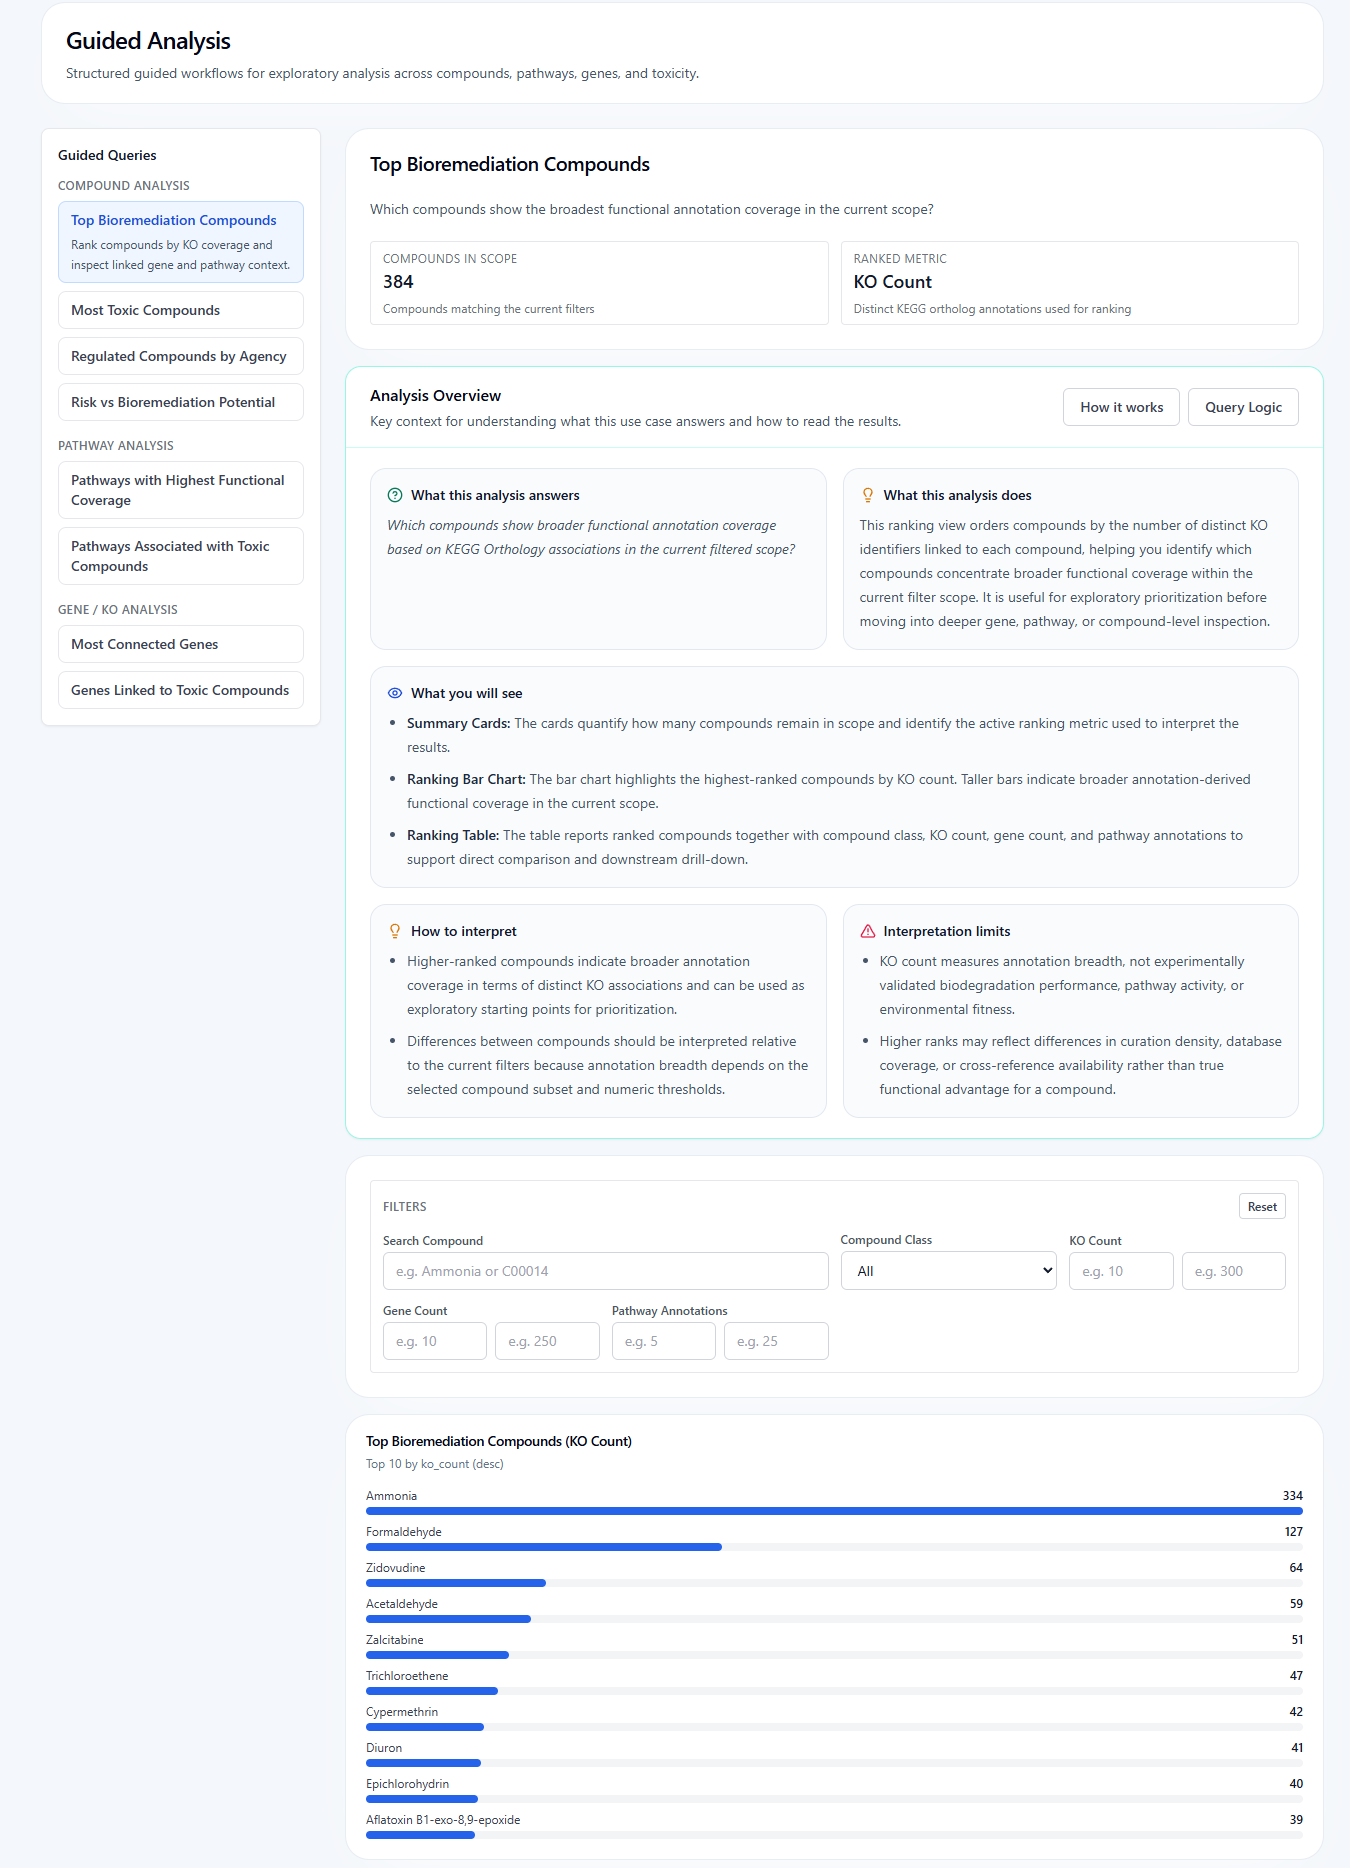
\includegraphics[width=\textwidth]
{figures/chapter_04/fig_04_guided_analysis.png}
\caption{Módulo de análises guiadas do BioRemPP Database Explorer. Cada caso
de uso reúne uma pergunta analítica, parâmetros de consulta, medidas
resumidas, visualização e tabela de resultados sob uma estrutura comum.}
\label{fig:c2-guided-analysis}
\end{figure}

% -----------------------------------------------------------------------------
\section{Resultados do componente}
\label{sec:c2-resultados}
% -----------------------------------------------------------------------------

O BioRemPP Database Explorer foi implementado como ambiente web de consulta à
versão do banco apresentada no Capítulo~\ref{cap:comp1}. Os resultados
compreenderam a implementação do ambiente de consulta, a disponibilização dos
módulos de exploração, a execução das análises guiadas. 

\subsection{Implementação do ambiente de consulta}

A versão avaliada reúne uma interface desenvolvida em React e TypeScript, uma
API interna baseada em Express e um banco SQLite destinado às operações da
aplicação. Esses elementos integram uma configuração conteinerizada que
combina o servidor, a interface compilada e a representação dos dados utilizada
durante a execução.

O banco SQLite contém as 12 tabelas requeridas pelo servidor e ocupa
15,77~MiB. A aplicação acessa esse arquivo em modo somente leitura, e as
consultas não dependem do carregamento dos arquivos CSV e XLSX publicados. O
SQLite constitui, portanto, a representação operacional do conteúdo descrito
no Capítulo~\ref{cap:comp1}, sem substituir os artefatos científicos
disponibilizados para distribuição e reutilização dos dados.

A API interna disponibiliza operações para os domínios de compostos, classes
químicas, genes e KOs, vias, toxicidade, metadados e análises guiadas. Na
avaliação da versão, as requisições aos módulos examinados retornam respostas
válidas e preservam os mecanismos de paginação, filtragem e recuperação das
entidades relacionadas.

\subsection{Módulos de exploração e navegação entre entidades}

Os cinco módulos previstos integram a aplicação: \textit{Compounds},
\textit{Compound Classes}, \textit{Genes / KO}, \textit{Pathways} e
\textit{Toxicity}. As Figuras~\ref{fig:c2-compounds-explorer} a
\ref{fig:c2-toxicity-explorer} apresentam as respectivas interfaces, enquanto
a Tabela~\ref{tab:c2-explorer-modules} sintetiza suas unidades de consulta e
as relações recuperadas.

O módulo de compostos recupera as anotações funcionais, as vias, as referências
institucionais e as predições toxicológicas associadas a cada CPD. O módulo de
classes químicas agrupa os compostos conforme o atributo utilizado na
interface. Os módulos de genes e KOs e de vias iniciam as consultas por
entidades funcionais, enquanto o módulo de toxicidade organiza os resultados
por combinação entre composto e endpoint.

A avaliação verifica a navegação entre as listagens e as páginas de detalhe a
partir das relações retornadas pela aplicação. Os registros de compostos
conduzem aos KOs, às vias e às predições toxicológicas associadas. No sentido
inverso, as consultas iniciadas por KO ou via recuperam os compostos
correspondentes. Os módulos de classes químicas e toxicidade também preservam
o acesso ao registro individual de cada composto.

A verificação examina a correspondência entre as entidades apresentadas nas
listagens e aquelas recuperadas nas páginas de detalhe. Seu escopo não abrange
uma avaliação de usabilidade com participantes nem a mensuração do desempenho
da interface sob carga concorrente.

\subsection{Análises guiadas e reprodutibilidade das consultas}

Foram implementados e executados os oito casos de uso descritos na
Tabela~\ref{tab:c2-guided-use-cases}. Quatro análises adotaram o composto como
unidade principal, duas organizaram os resultados por via e duas partiram de
genes e KOs. Todos os casos retornaram os resultados, as medidas resumidas e
as visualizações definidas nas respectivas configurações.

\begin{table}[htbp]
\centering
\caption{Execução dos grupos de análises guiadas do BioRemPP Database
Explorer.}
\label{tab:c2-guided-execution}
\small
\begin{tabularx}{\textwidth}{@{}p{3.1cm}p{2.5cm}X@{}}
\toprule
\textbf{Grupo}
& \textbf{Casos de uso}
& \textbf{Resultado da execução} \\
\midrule

Compostos
& UC1--UC4
& As quatro análises foram executadas e produziram os resumos, as
visualizações e as tabelas definidos para consultas centradas em compostos. \\

Vias
& UC5--UC6
& As duas análises foram executadas sobre as associações entre vias, KOs,
compostos e predições toxicológicas. \\

Genes e KOs
& UC7--UC8
& As duas análises foram executadas sobre as associações entre símbolos
gênicos, KOs, compostos e valores toxicológicos preditos. \\

\bottomrule
\end{tabularx}
\end{table}

As oito análises seguem a estrutura compartilhada apresentada na
Figura~\ref{fig:c2-guided-structure}. A aplicação processa as configurações
YAML para definir os parâmetros, as medidas resumidas, as visualizações e as
tabelas de cada caso de uso. A API organiza essas informações em um formato
comum, independentemente da entidade adotada como ponto de entrada.

A Figura~\ref{fig:c2-guided-analysis} exemplifica a interface correspondente.
Todos os casos de uso mantêm a mesma organização, composta pela seleção da
análise, definição dos parâmetros, apresentação das medidas resumidas,
visualização e tabela de resultados.

Cada caso de uso permanece associado a uma receita SQL versionada. As oito
receitas operam sobre a mesma versão do banco SQLite e reproduzem as unidades
de análise, os filtros, as agregações, as métricas principais e os critérios de
ordenação definidos pela aplicação. As diferenças relacionadas à paginação ou
à seleção dos campos apresentados permanecem restritas à projeção da resposta e
não modificam as operações analíticas.

A associação entre as especificações YAML e as receitas SQL registra tanto a
configuração utilizada pela interface quanto a consulta executada sobre o
banco. Essa organização possibilita repetir os procedimentos analíticos
independentemente das visualizações apresentadas pelo BioRemPP Database
Explorer.

\subsection{Verificação técnica e disponibilização}

A suíte automatizada executou 172 testes distribuídos em 53 arquivos, sem
falhas. As verificações abrangeram os módulos de exploração, as configurações
das análises guiadas, os componentes de visualização, as funções
compartilhadas e o comportamento esperado da interface.

A verificação de tipos, a análise estática e a compilação da aplicação foram
concluídas sem erros. A cobertura de testes atendeu aos limiares definidos
para linhas, instruções, funções e desvios condicionais. As oito
especificações YAML e as respectivas receitas analíticas também foram
validadas pelos procedimentos automatizados do projeto.

O perfil do banco SQLite foi verificado quanto à presença das estruturas
requeridas, à integridade do arquivo e ao limite de tamanho definido para o
ambiente de execução. A construção da imagem conteinerizada foi concluída, e
os serviços atingiram o estado saudável. As consultas realizadas no
contêiner reproduziram as respostas obtidas no ambiente local para os módulos
avaliados e para os oito casos de uso.

A Tabela~\ref{tab:c2-technical-verification} resume os resultados das
verificações realizadas sobre a versão avaliada.

\begin{table}[htbp]
\centering
\caption{Resultados das verificações técnicas do BioRemPP Database Explorer.}
\label{tab:c2-technical-verification}
\small
\begin{tabularx}{\textwidth}{@{}p{4.1cm}p{2.3cm}X@{}}
\toprule
\textbf{Verificação}
& \textbf{Resultado}
& \textbf{Evidência principal} \\
\midrule

Testes automatizados
& Aprovada
& 172 testes foram aprovados em 53 arquivos. \\

Cobertura de testes
& Aprovada
& Os limiares configurados para linhas, instruções, funções e desvios
condicionais foram atendidos. \\

Verificação de tipos
& Aprovada
& Nenhum erro de tipagem foi identificado. \\

Análise estática
& Aprovada
& Nenhuma violação bloqueante permaneceu no código avaliado. \\

Compilação da aplicação
& Aprovada
& A interface e o servidor foram compilados para o ambiente de produção. \\

Configurações das análises guiadas
& Aprovada
& As oito especificações YAML foram processadas e validadas. \\

Receitas SQL
& Aprovada
& As oito receitas reproduziram as métricas principais das análises
correspondentes. \\

Perfil do banco SQLite
& Aprovada
& O arquivo apresentou as 12 tabelas requeridas, integridade válida e
15,77~MiB. \\

Execução conteinerizada
& Aprovada
& A imagem foi construída, os serviços atingiram estado saudável e as
consultas de verificação retornaram respostas válidas. \\

\bottomrule
\end{tabularx}
\end{table}


Os elementos necessários à reprodução do Database Explorer foram mantidos no
repositório, incluindo o código-fonte, os arquivos de configuração, as
especificações YAML, as receitas SQL, a definição do ambiente conteinerizado e
a documentação. O uso dos identificadores CPD e KO preservou a
correspondência com as entidades adotadas no banco publicado.

O BioRemPP Database Explorer foi disponibilizado em
\url{https://bioinfo.imd.ufrn.br/bioremppdbx/}. O código-fonte encontra-se em
\url{https://github.com/BioRemPP/biorempp-dbx}, e a documentação está
disponível em
\url{https://biorempp-dbx.readthedocs.io/en/stable/}. O código foi distribuído sob a licença Apache~2.0, enquanto os dados
permaneceram disponíveis sob a licença CC~BY~4.0.

% -----------------------------------------------------------------------------
\section{Discussão do componente}
\label{sec:c2-discussao}
% -----------------------------------------------------------------------------

O BioRemPP Database Explorer não acrescenta novas evidências ao banco
integrado, mas modifica as condições de acesso às associações já
estabelecidas. Os arquivos publicados permanecem como referência versionada
para distribuição e reutilização, enquanto a aplicação permite consultar o
mesmo conteúdo sem manipulação direta da tabela central. A contribuição do
componente está na tradução da estrutura integrada em consultas iniciadas por
entidades químicas, funcionais e toxicológicas.

O uso de um banco SQLite atende ao perfil consultivo da aplicação. O
Database Explorer opera sobre dados previamente integrados e não recebe
alterações produzidas pelos usuários durante a execução. A representação
operacional permite aplicar filtros, ordenações, agregações e paginação sem
reprocessar os arquivos CSV e XLSX em cada requisição. A abertura do banco em
modo somente leitura também preserva o conteúdo materializado durante o uso
da interface. A separação entre os arquivos publicados e o SQLite mantém funções distintas
para os dois formatos. Os arquivos CSV e XLSX preservam o conteúdo científico
em uma forma adequada à distribuição, à citação e ao processamento externo. O
SQLite organiza as estruturas exigidas pelas consultas da aplicação e pode ser
reconstruído a partir da versão correspondente dos conjuntos de entrada. A
interface não se torna, portanto, a única forma de acesso ao banco BioRemPP. A API interna restringe o acoplamento entre a interface e a organização física
dos dados. Os módulos enviam os parâmetros da consulta e recebem respostas
estruturadas sem acessar diretamente o arquivo SQLite. Essa separação permite
alterar a apresentação dos resultados sem modificar a representação
científica publicada e concentra no servidor as regras de consulta
compartilhadas pelos diferentes módulos.

A organização dos exploradores por entidade permite formular consultas a
partir de diferentes pontos de entrada. O módulo de compostos parte do CPD,
enquanto os módulos de genes e KOs e de vias iniciam a consulta pela dimensão
funcional. Os módulos de classes químicas e toxicidade acrescentam recortes
voltados, respectivamente, ao agrupamento dos compostos e às predições por
endpoint. Essa organização operacionaliza a complementaridade entre CPD e KO
descrita no modelo do banco. A navegação entre listagens e páginas de detalhe mantém o contexto das
associações recuperadas. Um composto pode ser examinado em relação aos KOs,
vias, números EC, reações, referências institucionais e endpoints associados.
De forma recíproca, uma consulta iniciada por KO ou via permite recuperar os
compostos relacionados. Os módulos funcionam, assim, como diferentes acessos
ao mesmo conjunto de relações, e não como coleções independentes.


As contagens exibidas nos exploradores sintetizam a quantidade de associações
registradas para cada entidade. Elas permitem ordenar resultados e delimitar
conjuntos para inspeção, mas não medem expressão gênica, atividade enzimática,
completude de vias ou eficiência de degradação. Uma contagem elevada indica
maior amplitude de anotação no banco, condicionada às fontes integradas e aos
critérios de curadoria descritos no Capítulo~\ref{cap:comp1}.

As análises guiadas complementam a exploração baseada em filtros livres. Os
oito casos de uso formalizam perguntas recorrentes ao definir a unidade
analisada, os parâmetros aceitos, a métrica calculada e a forma de
apresentação. Essa definição reduz a variação decorrente da composição manual
de filtros e mantém explícito o procedimento aplicado a cada consulta. A implementação declarativa em YAML associa a pergunta analítica aos
parâmetros, às medidas resumidas, à visualização e aos limites de
interpretação. Alterações nesses elementos permanecem vinculadas à versão da
configuração correspondente. A definição da análise fica separada dos
componentes responsáveis por sua apresentação, o que permite distinguir
mudanças no procedimento analítico de modificações exclusivamente de interface.

As receitas SQL associadas aos casos de uso fornecem uma representação
executável das consultas. A repetição dos resultados depende da mesma versão
do SQLite, dos mesmos parâmetros e dos mesmos critérios para valores ausentes,
agregações e ordenação. A receita documenta o procedimento independentemente
da interface, enquanto o YAML registra como esse procedimento é parametrizado
e apresentado no Database Explorer. A reprodução das métricas principais pelas receitas SQL indica
correspondência entre as análises executadas pela aplicação e sua descrição
externa. Diferenças de paginação, seleção de campos ou apresentação de
subconjuntos não modificam necessariamente a operação analítica. Essas
diferenças precisam, contudo, permanecer documentadas quando a saída da
interface for comparada diretamente à consulta completa. Os casos de uso mantêm caráter exploratório. Os rankings baseados em KOs,
símbolos gênicos ou compostos descrevem relações presentes no banco e não
demonstram desempenho biológico. As análises que combinam anotações funcionais
e valores toxicológicos também não estabelecem causalidade entre genes, vias e
toxicidade. Os resultados permitem priorizar registros para inspeção, mas
exigem validação independente antes de sustentar conclusões experimentais.

A interpretação das predições toxicológicas depende do endpoint selecionado.
Cada endpoint descreve uma propriedade distinta e pode apresentar escala,
direção e significado próprios. Seus valores não devem ser combinados como uma
medida única de risco sem justificativa específica. As categorias exibidas
também não substituem ensaios experimentais ou avaliações formais de perigo. Os limiares calculados a partir do conjunto filtrado produzem classificações
relativas ao recorte analisado. No caso da análise que relaciona amplitude de
anotação gênica e toxicidade predita, a posição de um composto depende da
distribuição dos registros incluídos na consulta. A alteração dos filtros pode
modificar os limiares e a distribuição entre os quadrantes, que não
correspondem a classes permanentes dos compostos.

O escopo do Database Explorer permanece restrito à consulta do banco
integrado. O componente não processa dados ômicos submetidos pelos usuários,
não atualiza automaticamente as fontes externas e não realiza avaliação
regulatória individualizada. O processamento de amostras pertence ao serviço
de análise do ecossistema BioRemPP, enquanto decisões regulatórias exigem a
consulta às fontes oficiais e à legislação vigente.


A disponibilização do código-fonte, da documentação, das configurações YAML,
das receitas SQL e do ambiente conteinerizado fornece mecanismos concretos
para reprodução e reutilização. O uso de CPD e KO preserva a correspondência
com identificadores externos, enquanto o versionamento associa as consultas à
versão dos dados e do software. As licenças do código e do banco explicitam as
condições de uso dos respectivos artefatos.

Esses mecanismos apoiam aspectos dos princípios FAIR no escopo do Database
Explorer. A aplicação e a documentação ampliam o acesso ao conteúdo; CPD e KO
favorecem a interoperabilidade; as receitas SQL e as configurações versionadas
permitem repetir as consultas; e as licenças estabelecem as condições de
reutilização.

No ecossistema BioRemPP, o Database Explorer ocupa a camada de consulta direta
ao banco integrado. Os arquivos publicados preservam o conteúdo científico, o
Database Explorer permite examinar suas associações e o serviço de análise
aplica esse conhecimento a dados fornecidos pelos usuários. A contribuição
específica do componente consiste em converter o banco versionado em um
ambiente de consulta por entidades relacionadas, com procedimentos analíticos
explícitos e limites de interpretação definidos.

% =============================================================================
% =============================================================================
% CAPÍTULO 5 --- COMPONENTE 3: BIOREMPP WEB SERVICE (BWS)
% =============================================================================
% =============================================================================
\chapter{Componente 3: BioRemPP Web Service (BWS)}
\label{cap:comp3}

% -----------------------------------------------------------------------------
\section{Motivação do componente}
\label{sec:c3-motivacao}
% -----------------------------------------------------------------------------

O \gls{bws} responde a uma necessidade que o \gls{dbx} não atende: análise ativa contra dados do próprio usuário. Pesquisadores em biotecnologia ambiental frequentemente dispõem de perfis de anotação funcional derivados de sequenciamento (genoma, metagenoma, transcriptoma) e querem confrontá-los com o banco curado para inferir potencial de biorremediação, priorizar candidatos e projetar consórcios. Escrever código para essas análises impõe uma barreira que muitos pesquisadores de bancada não estão dispostos ou preparados a atravessar.

O \gls{bws} elimina essa barreira aceitando \gls{ko} profiles submetidos pelo usuário e processando-os através de oito módulos analíticos totalizando 56 casos de uso predefinidos, todos operando contra a mesma evidência integrada exposta pelo \gls{dbx}. O público-alvo é o pesquisador com dados próprios que quer aproveitar a curadoria \biorempp{} sem necessidade de programar.

% -----------------------------------------------------------------------------
\section{Arquitetura upload-based}
\label{sec:c3-arquitetura}
% -----------------------------------------------------------------------------

\escrever{Descrever a arquitetura em prosa técnica compacta: fluxo de submissão (upload de arquivo tabular contendo perfis KO por amostra), validação de entrada (mesma disciplina de contrato de parser do CLI, discutida no Cap 6), processamento server-side contra o banco integrado, apresentação de resultados. Mencionar que a arquitetura server-side permite computação mais intensiva que o browser sozinho poderia suportar (por exemplo, algoritmos combinatórios do módulo de assembly de consórcios).}

\begin{figure}[htbp]
\centering
\fbox{\parbox{0.85\textwidth}{\centering \todo{Figura 5.1 --- Diagrama de fluxo do BWS. Usuário $\rightarrow$ upload de arquivo KO $\rightarrow$ validação de contrato $\rightarrow$ merge contra banco integrado $\rightarrow$ processamento pelos módulos analíticos $\rightarrow$ apresentação de resultados. Anotar entradas e saídas de cada etapa.}\vspace{2em}}}
\caption{Arquitetura upload-based do \gls{bws}. Perfis \gls{ko} submetidos pelo usuário são validados, integrados contra o banco curado e processados através de oito módulos analíticos.}
\label{fig:c3-arquitetura}
\end{figure}

% -----------------------------------------------------------------------------
\section{Oito módulos analíticos e 56 casos de uso}
\label{sec:c3-modulos}
% -----------------------------------------------------------------------------

\reaproveitar{Trazer do draft anterior a descrição dos oito módulos analíticos (Seções 3.3.3 e 4.2 do original), atualizando terminologia para consistência com esta versão da tese e removendo qualquer conteúdo que se refira ao web browsing (que agora pertence ao \gls{dbx}, Capítulo~\ref{cap:comp2}).}

\escrever{Estruturar como oito subseções (5.3.1 a 5.3.8), uma por módulo, cada uma cobrindo: nome do módulo, pergunta que ele responde, tipos de entrada esperados, principais casos de uso oferecidos, tipo de output. Ao final, incluir tabela resumo.}

\subsection{Panorama geral}

\begin{table*}[htbp]
\centering
\caption{Panorama dos oito módulos analíticos do \gls{bws} totalizando 56 casos de uso.}
\label{tab:c3-modulos}
\small
\begin{tabular}{@{}rlrp{6cm}@{}}
\toprule
\textbf{\#} & \textbf{Módulo} & \textbf{UCs} & \textbf{Escopo analítico} \\
\midrule
1 & \todo{Nome do módulo 1}                     & \todo{n} & \todo{Escopo} \\
2 & \todo{Nome do módulo 2}                     & \todo{n} & \todo{Escopo} \\
3 & \todo{Nome do módulo 3}                     & \todo{n} & \todo{Escopo} \\
4 & \todo{Nome do módulo 4}                     & \todo{n} & \todo{Escopo} \\
5 & \todo{Nome do módulo 5}                     & \todo{n} & \todo{Escopo} \\
6 & \todo{Nome do módulo 6}                     & \todo{n} & \todo{Escopo} \\
7 & \todo{Nome do módulo 7}                     & \todo{n} & \todo{Escopo} \\
8 & \todo{Nome do módulo 8}                     & \todo{n} & \todo{Escopo} \\
\midrule
\textbf{Total} & & \textbf{56} & \\
\bottomrule
\end{tabular}
\end{table*}

\todo{Preencher a tabela com os nomes reais dos oito módulos e a distribuição dos 56 casos de uso entre eles. Como esses módulos são o coração diferencial do BWS, vale a pena dedicar prosa técnica robusta a cada um.}

% -----------------------------------------------------------------------------
\section{Métricas ecológico-funcionais}
\label{sec:c3-metricas}
% -----------------------------------------------------------------------------

\reaproveitar{Migrar da Seção 2.6 do draft original (que estava em Fundamentação Teórica) o conteúdo sobre métricas ecológicas aplicadas a dados funcionais. Reformular para descrever como cada métrica é implementada no BWS e para qual pergunta analítica ela responde.}

\subsection{Riqueza funcional}

\escrever{Definir riqueza funcional como contagem de KOs únicos anotados em uma amostra ou conjunto de amostras. Discutir sua interpretação como proxy para amplitude do repertório metabólico. Explicitar limitações (não considera abundância, não considera função ativa versus potencial genético).}

\subsection{Cobertura de compostos}

\escrever{Definir cobertura de compostos como fração de compostos prioritários endereçados pelos KOs anotados na amostra, ponderada ou não por número de vias/reações associadas. Discutir uso como score de potencial biodegradativo aplicado.}

\subsection{Completude de pathway}

\escrever{Definir completude como proporção de KOs esperados numa via específica que estão presentes na amostra. Discutir como isso permite distinguir vias parcialmente representadas de vias funcionalmente completas.}

\subsection{Guildas metabólicas}

\escrever{Discutir a atribuição de amostras a guildas metabólicas com base em padrões de riqueza funcional e cobertura. Utilidade para caracterização comparativa e para triagem de consórcios.}

\subsection{Otimização combinatória para design de consórcios}

\escrever{Descrever o algoritmo greedy set-cover implementado, sua complexidade, justificativa da abordagem greedy em vez de programação linear inteira (custo computacional vs qualidade da solução). Referenciar o módulo de assembly de consórcios do BWS.}

% -----------------------------------------------------------------------------
\section{Interoperabilidade com o banco integrado}
\label{sec:c3-interop}
% -----------------------------------------------------------------------------

O \gls{bws} consome a mesma release do banco integrado que o \gls{dbx}, garantindo consistência entre resultados obtidos nas duas ferramentas. A cada release do banco corresponde uma release do \gls{bws} que a incorpora; upgrades de versão do banco propagam-se para o \gls{bws} através do mesmo pipeline de deploy.

Essa consistência é auditável: perguntas exploratórias respondidas por navegação no \gls{dbx} produzem os mesmos números que perguntas analíticas equivalentes rodadas no \gls{bws}. Isso torna as duas ferramentas complementares em fluxo de trabalho: um pesquisador tipicamente começa pela navegação exploratória no \gls{dbx} para escolher escopo, e depois submete seus próprios dados ao \gls{bws} para análise dirigida.

% -----------------------------------------------------------------------------
\section{Resultados do componente}
\label{sec:c3-resultados}
% -----------------------------------------------------------------------------

\escrever{Reunir aqui: (i) screenshot da interface principal do BWS mostrando o fluxo de submissão; (ii) exemplo de output para pelo menos dois módulos representativos; (iii) discussão de escalabilidade (tamanho máximo de upload aceito, tempo típico de execução).}

% -----------------------------------------------------------------------------
\section{Status editorial}
\label{sec:c3-editorial}
% -----------------------------------------------------------------------------

Um manuscrito companheiro dedicado exclusivamente ao \gls{bws} está atualmente em revisão editorial no \gls{nar} Web Server Issue (referência de manuscrito NAR-00839-Web-S-2026.R1, Executive Editor Dr.~Dominik Seelow). Esse manuscrito complementa a descrição apresentada nesta tese, aprofundando aspectos que aqui recebem tratamento sintético.

% -----------------------------------------------------------------------------
\section{Discussão específica do componente}
\label{sec:c3-discussao}
% -----------------------------------------------------------------------------

O \gls{bws} atende a um perfil de usuário distinto tanto do \gls{dbx} quanto do \gls{cli} (Capítulo~\ref{cap:comp4}). Enquanto o \gls{dbx} serve pesquisadores que querem explorar o banco curado sem submeter dados próprios, e o \gls{cli} serve bioinformatas que operam em pipelines automatizados, o \gls{bws} atende o meio-termo: pesquisadores com dados próprios que preferem interface web a linha de comando.

A cobertura dos oito módulos totalizando 56 casos de uso é notável em amplitude, mas deve ser avaliada em relação ao público. Uma limitação a reconhecer é que a granularidade fina de opções pode representar barreira cognitiva para usuários novos: o próprio módulo de Guided Analysis do \gls{dbx} (Seção~\ref{sec:c2-guided}) foi projetado em parte para oferecer entrada mais gentil quando o pesquisador ainda não sabe qual dos 56 casos de uso do \gls{bws} melhor responde à sua pergunta.

\escrever{Adicionar parágrafo comparando o BWS com plataformas correlatas de análise funcional em bioinformática (MicrobiomeAnalyst, EnviPath, RemeDB) em termos de escopo analítico, complexidade de uso e integração com evidência regulatória.}


%% =============================================================================
% =============================================================================
% CAPÍTULO 6 --- COMPONENTE 4: BIOREMPP CLI
% =============================================================================
% =============================================================================
\chapter{Componente 4: BioRemPP CLI}
\label{cap:comp4}

% -----------------------------------------------------------------------------
\section{Motivação do componente}
\label{sec:c4-motivacao}
% -----------------------------------------------------------------------------

O quarto componente do ecossistema \biorempp{} atende ao perfil de usuário que opera em ambientes de linha de comando ou containers automatizados. Esse perfil --- tipicamente bioinformatas e engenheiros de dados científicos --- precisa não de uma interface amigável, mas de um cliente com contrato estrito de entrada e saída, rastreabilidade completa da execução e códigos de saída padronizados que permitam encadeamento em pipelines Snakemake, Nextflow ou similares.

O \gls{cli} preenche exatamente esse papel: um cliente Python distribuído via \gls{pypi} que expõe operações de anotação e relatório contra o banco integrado, com o mesmo rigor de reprodutibilidade que o pipeline de geração do banco (Capítulo~\ref{cap:comp1}) impõe à construção do artefato.

% -----------------------------------------------------------------------------
\section{Arquitetura do cliente}
\label{sec:c4-arquitetura}
% -----------------------------------------------------------------------------

O \gls{cli} organiza sua funcionalidade em seis comandos raiz: \texttt{annotate}, \texttt{report}, \texttt{database}, \texttt{config}, \texttt{info} e \texttt{completion}. O comando \texttt{annotate} executa o merge de perfis de entrada contra as bases integradas; \texttt{report} produz relatórios a partir de outputs prévios; \texttt{database} lida com operações de gerenciamento do artefato local; \texttt{config}, \texttt{info} e \texttt{completion} oferecem introspecção da configuração ativa, metadata do cliente e suporte a shell completion.

Opções globais uniformes complementam os comandos: níveis de verbosidade (\texttt{-v}, \texttt{-vv}, \texttt{-vvv}), modo silencioso (\texttt{-q}), configuração por arquivo (\texttt{--config}), controle de paralelismo (\texttt{--threads}), semente reproduzível (\texttt{--seed}), consulta de versão (\texttt{--version}) e citação (\texttt{--cite}). Esse conjunto de opções segue convenções bem estabelecidas em ferramentas bioinformáticas de linha de comando, reduzindo a curva de aprendizado para usuários habituados a operar em ambientes shell.

\subsection{Contrato estrito de parser}

O parser de entrada implementa contrato rígido para reduzir ambiguidade e evitar erros silenciosos. Metadata declarativa aparece em cabeçalho antes da primeira linha \texttt{>sample}, com prefixos convencionados \texttt{@dataset:*} e \texttt{@mode.*:*}. Comentários \texttt{\#} são permitidos apenas em cabeçalho. Whitespace inicial em linhas de dados é inválido. Linhas de dados sem cabeçalho \texttt{>sample} prévio falham. Pares duplicados \texttt{(sample, key)} falham. Essa disciplina garante que ambiguidades sejam sinalizadas ao usuário no momento da execução, em vez de propagarem-se para outputs silenciosamente incorretos.

% -----------------------------------------------------------------------------
\section{Quatro modos operacionais}
\label{sec:c4-modos}
% -----------------------------------------------------------------------------

O \gls{cli} implementa quatro modos operacionais que cobrem tipos distintos de dados ômicos que podem ser confrontados com o banco integrado (Tabela~\ref{tab:c4-modos}). Cada modo tem sua gramática de linha de dados, seu conjunto de metadata específica e suas regras próprias de validação.

\begin{table*}[htbp]
\centering
\caption{Modos operacionais do \gls{cli} \biorempp{}.}
\label{tab:c4-modos}
\small
\begin{tabular}{@{}lllp{5cm}@{}}
\toprule
\textbf{Modo} & \textbf{Chave} & \textbf{Gramática de linha} & \textbf{Metadata específica} \\
\midrule
\texttt{genomic}     & \texttt{ko}       & \texttt{K\textbackslash d\{5\}}          & (nenhuma) \\
\texttt{expression}  & \texttt{ko}       & \texttt{K\textbackslash d\{5\};value}    & \texttt{value\_type}, \texttt{missing\_value\_policy} \\
\texttt{reaction}    & \texttt{reaction} & \texttt{R\textbackslash d\{5\}}          & \texttt{analysis\_type}, \texttt{id\_namespace} \\
\texttt{enzymatic}   & \texttt{ec}       & \texttt{n.n.n.n} & \texttt{analysis\_type}, \texttt{id\_namespace} \\
\bottomrule
\end{tabular}
\end{table*}

O modo \texttt{genomic} aceita perfis de presença/ausência de \glspl{ko} agrupados por amostra, formato natural para saídas de KofamScan, KEGG BlastKOALA ou pipelines de anotação equivalentes sobre genomas ou \glspl{mag}. O modo \texttt{expression} estende essa gramática adicionando um valor numérico por \gls{ko}, apropriado para dados de expressão gênica (TPM, FPKM, contagens normalizadas) derivados de RNA-Seq. O modo \texttt{reaction} opera sobre identificadores de reação KEGG, servindo análises com viés metabolômico. O modo \texttt{enzymatic} opera sobre números EC, servindo análises com dados de anotação proteômica ou catalítica.

Essa cobertura de quatro modos torna o \gls{cli} genuinamente multi-ômico: um único cliente serve pesquisadores trabalhando com genômica, transcriptômica, metabolômica e informação enzimática, sempre confrontando-os contra o mesmo banco integrado.

\subsection{Estratégia de fan-out para o modo reaction}

O modo \texttt{reaction} implementa uma estratégia de fan-out sobre as bases integradas, executando o merge contra o subconjunto relevante de bases (BioRemPP, HADEG, KEGG) numa única invocação com \texttt{--database all}. Esse comportamento reduz o número de invocações necessárias em pipelines típicos e mantém a coerência de resultados através das bases.

% -----------------------------------------------------------------------------
\section{Sidecars e rastreabilidade}
\label{sec:c4-sidecars}
% -----------------------------------------------------------------------------

Para cada arquivo de output, o \gls{cli} gera um sidecar \texttt{<output\_file>.meta.json} contendo campos que documentam o contexto de execução completo (Tabela~\ref{tab:c4-sidecar}).

\begin{table}[htbp]
\centering
\caption{Campos principais do sidecar JSON gerado pelo \gls{cli} \biorempp{} para cada output.}
\label{tab:c4-sidecar}
\small
\begin{tabular}{@{}lp{7cm}@{}}
\toprule
\textbf{Campo} & \textbf{Conteúdo} \\
\midrule
\texttt{input\_mode}            & Modo operacional utilizado (genomic/expression/reaction/enzymatic) \\
\texttt{input\_metadata}        & Metadata declarativa do arquivo de entrada \\
\texttt{parse\_policy}          & Política de parsing aplicada \\
\texttt{parser\_contract\_version}     & Versão do contrato de parser \\
\texttt{metadata\_schema\_version}     & Versão do schema de metadata \\
\texttt{rows\_input}            & Número de linhas na entrada \\
\texttt{rows\_db}               & Número de linhas na base consultada \\
\texttt{rows\_merged}           & Número de linhas no output merged \\
\texttt{input\_sha256}          & Hash \gls{sha}-256 do arquivo de entrada \\
\texttt{database\_sha256}       & Hash \gls{sha}-256 da base consultada \\
\texttt{resolved\_paths}        & Caminhos absolutos resolvidos \\
\texttt{effective\_config}      & Configuração efetivamente aplicada \\
\bottomrule
\end{tabular}
\end{table}

O uso de hashes \gls{sha}-256 tanto do input quanto do banco garante que qualquer output pode ser reproduzido de forma bit-for-bit por um terceiro que disponha dos mesmos arquivos. Essa disciplina de rastreabilidade replica no nível do cliente o modelo de release imutável adotado no pipeline de geração do banco (Seção~\ref{sec:c1-snakemake}).

\begin{figure}[htbp]
\centering
\fbox{\parbox{0.85\textwidth}{\centering \todo{Figura 6.1 --- Fluxo de rastreabilidade do CLI. Input file $\rightarrow$ SHA-256 $\rightarrow$ merge $\rightarrow$ Output file + sidecar contendo hashes de input, database e output. Anotar como um terceiro pode reexecutar exatamente a mesma operação a partir do sidecar.}\vspace{2em}}}
\caption{Fluxo de rastreabilidade do \gls{cli} \biorempp{}: cada execução deixa um sidecar JSON com hashes \gls{sha}-256 que permitem reprodução bit-for-bit.}
\label{fig:c4-sidecars}
\end{figure}

% -----------------------------------------------------------------------------
\section{Exit codes e integração em pipelines}
\label{sec:c4-exitcodes}
% -----------------------------------------------------------------------------

Códigos de saída padronizados permitem que ferramentas de orquestração (Snakemake, Nextflow, Make, scripts shell) distingam categorias de falha e ajam apropriadamente sobre elas (Tabela~\ref{tab:c4-exitcodes}).

\begin{table}[htbp]
\centering
\caption{Códigos de saída do \gls{cli} \biorempp{}.}
\label{tab:c4-exitcodes}
\small
\begin{tabular}{@{}rl@{}}
\toprule
\textbf{Código} & \textbf{Significado} \\
\midrule
0   & Sucesso \\
1   & Erro geral \\
2   & Uso inválido (linha de comando) \\
3   & Erro de entrada \\
4   & Erro de saída \\
5   & Erro de base de dados \\
6   & Erro de validação \\
7   & Erro de configuração \\
8   & Erro de dependência \\
130 & Interrompido pelo usuário (SIGINT) \\
\bottomrule
\end{tabular}
\end{table}

Essa categorização permite estratégias diferenciadas de retry, logging e alerta em pipelines: erros de entrada (código 3) podem ser tratados diferentemente de erros de base (código 5) ou de erros de configuração (código 7). O padrão segue convenções amplamente adotadas em ferramentas bioinformáticas mainstream.

\subsection{Modo dry-run}

Todas as operações \texttt{annotate} suportam a flag \texttt{--dry-run}, que executa apenas a validação de contrato sem produzir outputs. Isso permite verificar preventivamente a integridade de metadata e linha de comando antes de iniciar processamento potencialmente longo.

\subsection{HTML reporting unificado}

Quando o output solicitado é HTML (\texttt{--format html}), o \gls{cli} gera uma pasta unificada \texttt{runs/<run\_id>/} contendo o relatório principal (\texttt{report.html}), sumário JSON (\texttt{report\_summary.json}), auditoria (\texttt{report\_audit.json}) e manifesto de execução (\texttt{run\_manifest.json}). Essa estrutura permite compartilhar um único artefato consolidado que inclui tanto o relatório visualmente navegável quanto os metadados que documentam sua produção.

\subsection{Compressão}

Outputs tabulares (\texttt{csv}, \texttt{tsv}) e JSON suportam compressão gzip via flag \texttt{--compress}, produzindo arquivos \texttt{.gz}. A combinação \texttt{--format html --compress} é intencionalmente inválida (código de saída 2), evitando a produção de arquivos HTML comprimidos que não seriam diretamente renderizáveis por browsers.

% -----------------------------------------------------------------------------
\section{Distribuição e requisitos}
\label{sec:c4-distribuicao}
% -----------------------------------------------------------------------------

O \gls{cli} é distribuído via \gls{pypi} sob o nome \texttt{biorempp}, instalável via \texttt{pip install biorempp}. A versão atual (v0.14.0) implementa os quatro modos com validação completa. Requisitos de runtime incluem Python 3.10, 3.11 ou 3.12, com \texttt{pandas} 2.x como dependência tabular principal. Geração de relatórios HTML requer \texttt{plotly} como dependência do runtime.

\todo{Atualizar a versão citada aqui conforme o release estável for publicado. A v0.14.0-beta-mvp mencionada no README interno pode ser substituída por versão sem sufixo beta antes da defesa da tese.}

% -----------------------------------------------------------------------------
\section{Resultados do componente}
\label{sec:c4-resultados}
% -----------------------------------------------------------------------------

\escrever{Reunir aqui: (i) exemplos de execução para cada um dos quatro modos com entradas mínimas válidas (baseados nos exemplos do README); (ii) exemplo de sidecar gerado, mostrando os campos populados; (iii) benchmark de performance sobre entradas de tamanho variável (opcional se não houver dados sistemáticos); (iv) cobertura de testes automatizados atual.}

\reaproveitar{Trazer da Seção 4.3 do draft anterior o conteúdo sobre performance e escalabilidade do CLI, se aplicável.}

% -----------------------------------------------------------------------------
\section{Discussão específica do componente}
\label{sec:c4-discussao}
% -----------------------------------------------------------------------------

O \gls{cli} completa o triplo canal de acesso ao banco integrado (\gls{dbx}, \gls{bws}, \gls{cli}), atendendo o perfil de usuário mais técnico. Sua contribuição diferencial não está na análise em si --- que pode ser executada equivalentemente via \gls{bws} --- mas em três propriedades operacionais que a interface web não pode oferecer: integrabilidade em pipelines automatizados, rastreabilidade bit-for-bit via sidecars com hashes e execução em ambientes onde interfaces gráficas não estão disponíveis (containers, clusters HPC, notebooks Jupyter em ambientes remotos).

A disciplina de contrato estrito de parser e a padronização de exit codes refletem uma decisão de posicionar o \gls{cli} como membro de primeira classe do ecossistema bioinformático mainstream, não como afterthought de linha de comando anexado ao BWS. Ferramentas amplamente adotadas na comunidade --- \texttt{samtools}, \texttt{bcftools}, \texttt{bedtools}, \texttt{seqkit} --- seguem convenções similares, e a adoção dessas convenções pelo \gls{cli} \biorempp{} facilita sua incorporação em pipelines existentes sem fricção conceitual para os usuários.

O status atual do \gls{cli} como release v0.14 (pré-estável) reflete o estágio de maturação do componente. Elementos ainda em consolidação (por exemplo, a finalização formal do modo enzimático via decision gate D20 e o empacotamento de documentação de release-readiness) estão documentados no repositório e devem ser resolvidos antes da versão estável 1.0.


% =============================================================================
% =============================================================================
% CAPÍTULO 7 --- DISCUSSÃO INTEGRADA E CONCLUSÕES
% =============================================================================
% =============================================================================
\chapter{Discussão integrada e conclusões}
\label{cap:conclusao}

% -----------------------------------------------------------------------------
\section{O ecossistema como unidade coerente}
\label{sec:c7-ecossistema}
% -----------------------------------------------------------------------------

Os quatro componentes apresentados nos Capítulos~\ref{cap:comp1} a~\ref{cap:comp4} não são artefatos independentes que compartilham uma marca; são um ecossistema integrado que compartilha uma decisão editorial (compound-centricidade orientada a prioridade regulatória) e uma base de evidência (o banco integrado). Um mesmo pesquisador transita naturalmente entre eles conforme a natureza da pergunta muda: começa navegando o \gls{dbx} para escolher escopo de compostos e classes químicas relevantes; submete seus perfis \gls{ko} ao \gls{bws} para análise dirigida contra os compostos priorizados; integra o \gls{cli} no pipeline de análise batch para automação; e retorna eventualmente ao \gls{dbx} para inspeção de detalhes específicos surgidos das análises anteriores.

Essa fluidez de transição é resultado do compartilhamento explícito de artefatos e identificadores. Resultados obtidos no \gls{bws} usam os mesmos identificadores \gls{ko}, \gls{cpd}, \gls{ec} que aparecem no \gls{dbx}; sidecars produzidos pelo \gls{cli} referenciam a mesma release do banco que o \gls{dbx} carrega no SQLite runtime. Não há tradução de identificadores entre componentes, e não há inconsistências entre resultados obtidos por caminhos diferentes.

% -----------------------------------------------------------------------------
\section{Contribuições consolidadas}
\label{sec:c7-contribuicoes}
% -----------------------------------------------------------------------------

As contribuições do trabalho podem ser organizadas em três eixos.

\subsection{Contribuição científica}

A unificação entre priorização regulatória e evidência funcional multi-fonte em torno de compostos ambientalmente prioritários, apresentada como decisão editorial deliberada e não como agregação exaustiva, é a contribuição científica central do trabalho. Nenhum recurso público disponível até o momento oferece essa combinação em arquitetura compound-centric, e a demanda por ela é sustentada pela crescente pressão regulatória sobre poluentes prioritários combinada à ausência de infraestrutura de monitoramento no nível de ômicas funcionais que caracterize os mecanismos moleculares relevantes para mitigação.

\subsection{Contribuição metodológica}

A arquitetura dual de validação (KEGG-anchored embutida no DAG Snakemake mais Great Expectations release-level em projeto separado) é uma contribuição metodológica autônoma ao campo de engenharia de dados científicos. A separação clara entre fidelidade de conteúdo (validação KEGG-anchored) e conformidade estrutural com estabilidade histórica (validação Great Expectations) resolve, em nossa leitura, uma tensão que fica frequentemente implícita em pipelines de bancos curados. A publicação da arquitetura completa, incluindo a suite pytest que testa o próprio validador, oferece à comunidade um padrão de referência replicável.

\subsection{Contribuição tecnológica}

O modelo de ecossistema modular composto por quatro componentes interoperáveis, atendendo perfis de usuário distintos com o mesmo banco integrado, contrasta com o padrão predominante em bioinformática de biorremediação de recursos monolíticos (ou banco baixável, ou interface web fechada, ou CLI standalone). A demonstração de que os três canais de acesso podem coexistir consistentemente, cada um otimizado para seu perfil de uso, oferece um padrão de arquitetura aplicável a outros domínios de curadoria.

% -----------------------------------------------------------------------------
\section{Posicionamento no estado da arte}
\label{sec:c7-posicionamento}
% -----------------------------------------------------------------------------

Comparado a plataformas correlatas (enviPath, PlasticDB, mibPOPdb, RemeDB, EAWAG-BBD, MicrobiomeAnalyst, DRAM, METABOLIC), o ecossistema \biorempp{} ocupa um nicho específico caracterizado por cinco propriedades cuja combinação, até onde temos conhecimento, não é oferecida por nenhum recurso individual (Tabela~\ref{tab:c7-comparacao}).

\begin{table*}[htbp]
\centering
\caption{Posicionamento do ecossistema \biorempp{} frente a recursos correlatos em bioinformática de biorremediação.}
\label{tab:c7-comparacao}
\small
\begin{tabular}{@{}lccccc@{}}
\toprule
\textbf{Recurso} & \textbf{Comp-centric} & \textbf{Multi-fonte} & \textbf{Regulatório} & \textbf{Toxicológico} & \textbf{Multi-canal} \\
\midrule
enviPath        & Não & Parcial & Não & Não & Web \\
PlasticDB       & Sim & Parcial & Não & Não & Web \\
mibPOPdb        & Sim & Não     & Parc. & Não & Web \\
RemeDB          & Não & Não     & Não & Não & CLI \\
EAWAG-BBD/PPS   & Não & Não     & Não & Não & Web \\
MicrobiomeAnalyst & Não & N/A   & Não & Não & Web \\
DRAM            & Não & N/A     & Não & Não & CLI \\
\biorempp{}     & Sim & Sim     & Sim & Sim & Web+Web+CLI \\
\bottomrule
\end{tabular}
\end{table*}

A leitura da tabela não é de superioridade absoluta, mas de complementaridade estrutural: cada recurso listado cumpre bem seu propósito de projeto, e o \biorempp{} não substitui nenhum deles. A contribuição do ecossistema \biorempp{} é ocupar um vazio metodológico deixado pela ausência de plataforma que combinasse simultaneamente as cinco propriedades listadas.

% -----------------------------------------------------------------------------
\section{Aplicações retrospectivas do ecossistema}
\label{sec:c7-aplicacoes}
% -----------------------------------------------------------------------------

O grupo de pesquisa responsável pelo \biorempp{} produziu três estudos peer-reviewed que utilizaram a evidência integrada que o ecossistema hoje expõe, demonstrando retrospectivamente o valor prático da infraestrutura para pesquisa aplicada em biorremediação industrial. Os três estudos são apresentados aqui como demonstração da utilidade do ecossistema, não como resultados originais da tese.

\subsection{Caracterização de nova subespécie hidrocarbonoclástica}

\citet{freitas2023acinetobacter} caracterizaram uma nova subespécie de \textit{Acinetobacter baumannii} isolada de reservatórios de petróleo brasileiros com especialização em degradação de hidrocarbonetos perigosos. A caracterização genômica e fenotípica beneficiou-se da consolidação de anotações funcionais e classificações regulatórias sobre os substratos-alvo, exatamente o tipo de análise que o \biorempp{} organiza sistematicamente.

\subsection{Integração transcriptômica e metatranscriptômica de consórcio industrial}

\citet{silvaportela2024consortium} integraram perfis transcriptômicos e metatranscriptômicos de um consórcio bacteriano degradador de resíduos oleosos. O consórcio caracterizado teve sua composição protegida por patente e encontra-se em uso operacional, ilustrando trajetória translacional que o ecossistema \biorempp{} apoia com evidência de referência.

\todo{Se o número da patente estiver publicamente disponível, incluir a referência aqui em nota de rodapé para reforçar a maturidade tecnológica do trabalho.}

\subsection{Descrição de novas espécies de \textit{Ochrobactrum}}

\citet{freitas2025ochrobactrum} reportaram a caracterização genômica e fenotípica de novas espécies de \textit{Ochrobactrum} isoladas de reservatórios brasileiros de petróleo. Como no caso anterior, a análise de potencial biodegradativo dessas espécies apoiou-se em confrontação de anotações funcionais com evidência integrada organizada por classes químicas ambientalmente relevantes.

\subsection{Síntese das aplicações retrospectivas}

Em conjunto, os três estudos cobrem três eixos analíticos distintos que o ecossistema \biorempp{} agora sistematiza publicamente: caracterização genômica de novas espécies e subespécies, integração multi-ômica funcional, e translação industrial com proteção de propriedade intelectual. Essa cobertura empírica sustenta a viabilidade de aplicação do ecossistema em contextos reais de pesquisa e desenvolvimento.

% -----------------------------------------------------------------------------
\section{Limitações}
\label{sec:c7-limitacoes}
% -----------------------------------------------------------------------------

Cinco limitações merecem menção explícita.

\textbf{Limitações inerentes a análises \textit{in silico}.} O ecossistema oferece triagem computacional que não substitui validação experimental. Predições de potencial biodegradativo devem ser tratadas como hipóteses a serem testadas em bancada, não como conclusões de eficácia.

\textbf{Dependência da qualidade da anotação upstream.} A análise no \gls{bws} e no \gls{cli} opera sobre anotações \gls{ko} produzidas por ferramentas externas (KofamScan, BlastKOALA, eggNOG-mapper). A qualidade das inferências de biorremediação é limitada pela qualidade dessa anotação upstream.

\textbf{Cobertura limitada de compostos.} O foco em compostos formalmente regulados por sete frameworks internacionais é decisão editorial deliberada (Seção~\ref{sec:c1-motivacao}), mas exclui compostos ambientalmente relevantes que ainda não foram objeto de listagem regulatória. Contaminantes emergentes cuja regulamentação está em processo de definição podem estar sub-representados até que sejam incorporados formalmente.

\textbf{Predições toxicológicas como screening.} As predições \gls{toxcsm} são \textit{screening tools}, não substitutos de medidas experimentais de toxicidade. Priorização baseada nessas predições deve ser validada experimentalmente antes de conclusões regulatórias ou de saúde pública.

\textbf{Status pré-estável do \gls{cli}.} A versão atual do \gls{cli} é rotulada v0.14 e permanecerá pré-estável até a conclusão de elementos de hardening documentados no repositório. Usuários que integram o \gls{cli} em pipelines produtivos devem pinar a versão utilizada.

% -----------------------------------------------------------------------------
\section{Perspectivas}
\label{sec:c7-perspectivas}
% -----------------------------------------------------------------------------

\subsection{Expansão da base}

Frameworks regulatórios adicionais (Ecolabel, REACH SVHC, listas nacionais adicionais) podem ser incorporados sem alteração arquitetural, apenas por expansão do vocabulário controlado \texttt{referenceAG}. Novos endpoints toxicológicos podem ser integrados por atualização da fonte ToxCSM ou por adição de fontes complementares (T3DB, ProTox-II).

\subsection{Integração multi-ômica expandida}

Suporte formal para dados proteômicos e metabolômicos ampliaria a cobertura do \gls{cli} para além dos quatro modos atuais. Integração com padrões emergentes de dados metagenômicos (Anvi'o, GTDB-Tk) reduziria fricção para pesquisadores em microbiomas ambientais.

\subsection{Modelos preditivos}

Modelos de aprendizado de máquina treinados sobre a evidência integrada poderiam prever capacidade biodegradativa a partir de perfis genômicos parciais, oferecendo alternativa quantitativa às métricas ecológicas do \gls{bws}.

\subsection{Sustentabilidade a longo prazo}

Assegurar manutenção continuada por período de cinco anos requer estratégia explícita para atualização periódica das fontes upstream, resposta a mudanças em contratos regulatórios e evolução das dependências de software. O uso de containers Docker versionados, workflows Snakemake reproducíveis e testes automatizados fornecem base técnica sólida, mas exigem alocação continuada de recursos humanos.

% -----------------------------------------------------------------------------
\section{Considerações finais}
\label{sec:c7-final}
% -----------------------------------------------------------------------------

Esta tese apresentou o \biorempp{} como ecossistema integrado de bioinformática para análise funcional e integração multi-ômica orientada a compostos prioritários para biorremediação. Os quatro componentes documentados (banco integrado com pipeline reprodutível e validação dupla; \gls{dbx} para navegação read-only; \gls{bws} para análise upload-based; \gls{cli} para integração em pipelines automatizados) formam um recurso publicamente disponível, licenciado abertamente e alinhado aos princípios \gls{fair}, oferecendo à comunidade científica uma plataforma que unifica evidências até então dispersas em torno da unidade analítica que a política ambiental e a saúde pública tratam como central: o composto regulado.

A contribuição principal do trabalho não está no aumento de escopo de qualquer das fontes constituintes, e sim na organização coerente dessa evidência em torno de uma decisão editorial compound-centric orientada a prioridade regulatória, servida através de canais complementares desenhados para os diferentes perfis técnicos da comunidade que faz uso desses dados. As três aplicações retrospectivas discutidas na Seção~\ref{sec:c7-aplicacoes} sustentam empiricamente a utilidade prática do ecossistema em pesquisa aplicada industrial, e as perspectivas apresentadas na Seção~\ref{sec:c7-perspectivas} indicam trajetória de evolução coerente com a sustentabilidade a longo prazo exigida de recursos de bioinformática.



% =============================================================================
% REFERENCIAS
% =============================================================================
\bibliographystyle{abntex2-num}
\bibliography{referencias}

% =============================================================================
% APÊNDICES
% =============================================================================
\appendix

% -----------------------------------------------------------------------------
\chapter{Esquema completo da base de dados integrada}
\label{ape:esquema-db}
% -----------------------------------------------------------------------------

\escrever{Este apêndice complementa a Tabela~\ref{tab:c1-schema} do corpo principal com detalhes exaustivos que seriam excessivos no capítulo. Incluir:}

\begin{itemize}
    \item Diagrama entidade-relacionamento mostrando as junções entre as quatro fontes constituintes (referenciar Figura~\ref{fig:c1-dualaxis} do corpo principal ou reproduzir versão expandida aqui).
    \item Dicionário de dados completo das 11 colunas da tabela core: nome do campo, tipo, obrigatoriedade, formato esperado, vocabulário controlado (quando aplicável), exemplos de valores.
    \item Lista completa das 12 classes químicas com contagens e exemplos.
    \item Lista completa dos nove códigos de agência com descrição e URL de referência oficial.
    \item Lista das 206 famílias de atividade enzimática (pode ser tabela longa dividida em páginas).
    \item Exemplos de registros representativos (2-3 exemplos ilustrando padrões típicos).
\end{itemize}

\todo{Elaborar este apêndice na fase final da tese, quando o schema estiver 100\% consolidado.}

% -----------------------------------------------------------------------------

\chapter{Código-fonte e disponibilidade}
\label{ape:codigo-fonte}
% -----------------------------------------------------------------------------

Todos os artefatos que compõem o ecossistema \biorempp{} são publicamente disponíveis nos seguintes canais:

\begin{description}
    \item[Organização GitHub] \url{https://github.com/BioRemPP}
    \item[Repositório do banco e pipeline] \todo{URL do repositório específico}
    \item[Repositório do \gls{dbx}] \todo{URL do repositório específico}
    \item[Repositório do \gls{bws}] \todo{URL do repositório específico}
    \item[Repositório do \gls{cli}] \todo{URL do repositório específico}
    \item[Repositório do validador Great Expectations] \todo{URL do repositório específico}
    \item[Zenodo (banco integrado v1.1.0)] \url{https://doi.org/10.5281/zenodo.18905195}
    \item[PyPI (\gls{cli})] \todo{URL específica do PyPI package}
    \item[\gls{dbx} em produção] \todo{URL institucional confirmada}
    \item[\gls{bws} em produção] \todo{URL institucional confirmada}
\end{description}

\textbf{Licenças:} código-fonte de todos os componentes sob Apache License 2.0; dados curados do banco integrado sob Creative Commons Attribution 4.0 International (CC BY 4.0).

\textbf{Instalação do \gls{cli}:}
\begin{lstlisting}[language=bash]
pip install biorempp
biorempp --version
biorempp --cite
\end{lstlisting}

\textbf{Requisitos de runtime do \gls{cli}:} Python 3.10, 3.11 ou 3.12; pandas 2.x; plotly (opcional, requerido apenas para geração de relatórios HTML).

% -----------------------------------------------------------------------------

\chapter{Comprovantes de submissão editorial}
\label{ape:comprovantes}
% -----------------------------------------------------------------------------

\escrever{Este apêndice reúne comprovantes de trâmites editoriais relacionados à publicação dos componentes do ecossistema:}

\begin{itemize}
    \item Comprovante de submissão do manuscrito companheiro do \gls{bws} ao \gls{nar} Web Server Issue (referência de manuscrito NAR-00839-Web-S-2026.R1), incluindo carta de submissão, histórico editorial e status atual de revisão.
    \item Comprovante da consulta de pré-submissão ao \gls{nar} Database Issue relativa ao \gls{dbx} e resposta editorial recebida (redirecionamento para \textit{Database (Oxford)}).
    \item Comprovante de depósito da release v1.1.0 no Zenodo (certificado de DOI).
    \item Comprovantes de participação em congressos onde o ecossistema \biorempp{} foi apresentado.
\end{itemize}

\todo{Reunir e digitalizar esses comprovantes na fase final da tese, verificando com a secretaria do PPgBioinfo/UFRN quais formatos são aceitos.}



\end{document}
